\documentclass[12pt,a4paper]{report}

% English
\usepackage[english]{babel} % English language setting
\usepackage[utf8]{inputenc} % Unicode text
\usepackage[T1]{fontenc} % German 'Umlaute'
\usepackage{textcomp} % Euro
\usepackage[hyphens]{url}
\usepackage{amsmath} % Advanced mathematical notation
\usepackage{amssymb} % Symbols
\usepackage{emptypage} % Empty pages are now actually empty
\usepackage{caption} % Better image and table captions
\usepackage{varwidth} % Used for the custom captions
\DeclareCaptionFormat{centered}{%
  % #1: label (e.g. "Table 1")
  % #2: separator (e.g. ": ")
  % #3: caption text
  \begin{varwidth}{\linewidth}
    #1#2#3%
  \end{varwidth}
}
\captionsetup{format=centered} % Global activation of the custom captions

\usepackage{xcolor}
\usepackage[tikz]{bclogo}
\usepackage[framemethod=tikz]{mdframed}
\usepackage{lipsum}
\usepackage[many]{tcolorbox}
\newtcolorbox{highlightbox}[1][]{
  breakable,
  freelance,
  title=#1,
  colback=white,
  colbacktitle=white,
  coltitle=black,
  fonttitle=\bfseries,
  bottomrule=0pt,
  boxrule=0pt,
  colframe=white,
  overlay unbroken and first={
  \draw[black,line width=3pt]
    ([xshift=5pt]frame.north west) --
    (frame.north west) --
    (frame.south west);
  \draw[black,line width=3pt]
    ([xshift=-5pt]frame.north east) --
    (frame.north east) --
    (frame.south east);
  },
  overlay unbroken app={
  \draw[black,line width=3pt,line cap=rect]
    (frame.south west) --
    ([xshift=5pt]frame.south west);
  \draw[black,line width=3pt,line cap=rect]
    (frame.south east) --
    ([xshift=-5pt]frame.south east);
  },
  overlay middle and last={
  \draw!black,line width=3pt]
    (frame.north west) --
    (frame.south west);
  \draw[black,line width=3pt]
    (frame.north east) --
    (frame.south east);
  },
  overlay last app={
  \draw[black,line width=3pt,line cap=rect]
    (frame.south west) --
    ([xshift=5pt]frame.south west);
  \draw[black,line width=3pt,line cap=rect]
    (frame.south east) --
    ([xshift=-5pt]frame.south east);
  },
}

% Fonts, with all the options
\usepackage[bitstream-charter]{mathdesign}
\usepackage[scaled=.96]{helvet}
\usepackage[scaled=.75]{beramono}
\usepackage{microtype}

% Images and listings
\usepackage{graphicx} % images
\usepackage{subfig} % sub-figures
\usepackage{wrapfig} % wrapping figures
\usepackage{listings} % better source code listings
\usepackage[algoruled,lined,linesnumbered,commentsnumbered]{algorithm2e} % algorithms
\usepackage{tabularx} % better tables
\usepackage{diagbox} % diagonally split table cells
\usepackage{multirow}
\usepackage{hhline}
\usepackage{enumitem}
\usepackage{array}
\usepackage{booktabs}
\usepackage{url}
\usepackage{forest}
\graphicspath{ {figures/} }

% Page layout
\usepackage[paper=a4paper,width=14cm,left=35mm,height=22cm]{geometry}
\usepackage{setspace}
\usepackage[htt]{hyphenat}
\usepackage{sectsty}
\linespread{1.5}
\subsubsectionfont{\large}

% Page markers
\newcommand{\phv}{\fontfamily{phv}\fontseries{m}\fontsize{10}{12}\selectfont}
\usepackage{fancyhdr} % nicer header and footer
\pagestyle{fancy}
\renewcommand{\chaptermark}[1]{\markboth{#1}{}}
\fancyhead[L]{\phv \nouppercase{\leftmark}}
\fancyhead[R]{\phv \thepage}
% rather not use anything for the footer
\fancyfoot[C]{\ } % no page count in the bottom
%\fancyfoot[R]{\textsf{\small Software Engineering MS}}

% Share the sources
\usepackage{bibtopic}

% Special packages
\usepackage{epigraph}
\setlength{\epigraphrule}{0pt} % no divider
\usepackage{csquotes}

% Some extra styles
\usepackage{soul}
\newcommand*\strikethrough{\st}

% Hyperlink everything
\usepackage{hyperref}
\hypersetup{
    colorlinks=true,
    linkcolor=black,
    citecolor=black,
    filecolor=black,
    urlcolor=black,
}
\urlstyle{same}

% Hyphenations
\hyphenation{non-neg-li-gi-ble}

\newcommand*\rot{\rotatebox{90}}
\newcolumntype{Y}{>{\centering\arraybackslash}X}

% Wikipedia-style "citation needed" macro
\newcommand{\cn}[1][]{\textsuperscript{\color{red} ~[citation needed]~}}

% UvA logo and text
\newcommand{\uva}{
	\begin{tabular}{r l}
		\multirow{2}{*}{
\includegraphics[height=65pt]{uva.pdf}}
		&\textsc{\Large Universiteit van Amsterdam}\\
		&\textsc{\small Faculteit der Natuurwetenschappen, Wiskunde en Informatica}\\
		&\textsc{\small Master Software Engineering}
	\end{tabular}
}

% Code markup
\newcommand{\code}[1]{\texttt{#1}}


\newcommand{\studyprogramme}{Software Engineering}
\newcommand{\degreetype}{Master of Science}
\newcommand{\thesistitle}{
Toward automatic decomposition of monolithic software into microservices
}
\newcommand{\thesissubtitle}{
Conception of a methodology and its exemplary implementation
}
\newcommand{\thesisauthor}{Jakob L{\"o}hnertz}
\newcommand{\thesisdate}{31/01/2020}
\newcommand{\thesislocation}{Amsterdam}
\newcommand{\firstmarker}{Dr.\ Ana Oprescu}
\newcommand{\secondmarker}{MSc.\ Stephan Schroevers}
\newcommand{\hostorganization}{Picnic B.V.}

\begin{document}




\begin{titlepage}
  \begin{center}
    \parbox[c]{\textwidth}{\uva}
    \\[2.5cm]
    {\LARGE Thesis} \\[0.35cm]
    {\begin{spacing}{1} to obtain the academic degree \\[0.5cm] \end{spacing}}
    {\begin{spacing}{1} \large \textbf{\degreetype} \\[1.5cm] \end{spacing}}
    \rule{\textwidth}{1pt} \\[0.55cm]
    {\begin{spacing}{1.15} \huge \bfseries \thesistitle \\[0.35cm] \end{spacing}}
    {\begin{spacing}{1.15} \bfseries \thesissubtitle \\[0.60cm] \end{spacing}}
    \rule{\textwidth}{1pt}
    \\[1.5cm]
    \begin{tabular}{l l}
      Author & \thesisauthor \\
      Research supervisor & \firstmarker \\
      Host supervisor & \secondmarker \\
      Host organization & \hostorganization \\
    \end{tabular}
  \end{center}
\end{titlepage}
\cleardoublepage

\thispagestyle{empty}
\section*{Affidavit}
I hereby declare that I have
\begin{itemize}
\item independently prepared this thesis,
\item not used any other sources than those indicated,
\item identified as such, either verbatim or according to the content, any parts taken from external works, pictorial representations and the like
\item not made use of any unauthorized external help.
\end{itemize}

\vspace{6em}
\noindent\begin{tabular}{p{0.37\textwidth}p{0.56\textwidth}}
\thesislocation, \thesisdate  & \rule{0.56\textwidth}{0.5pt}\\
              & \makebox[1cm]{\ } \thesisauthor
\end{tabular}

\vfill

\cleardoublepage

\raggedbottom


\thispagestyle{empty}
\section*{Acknowledgments}
First and foremost, I want to thank my family and my friends here in Amsterdam and back at home in Germany.
They provided support, proofreading, and fun times during this entire summer.
Specific thanks go to my two best friends Jean Marcel Petry and Eric Richter, who is also my flatmate,
who always have an open ear, no less during the thesis period.
Additionally, I specifically want to thank Christian Stuart, Sander Meester, and Changhun Yun
who aided me relentlessly when I got sick toward the end of the writing period for multiple weeks.
In the same vein, my family massively helped in getting healthy again.
Their daily support comforted me a lot and although I could not turn the thesis in, in the end of August
as originally planned, they sped up the time it took me to get back on track immensely.
Moreover, I want to thank Moustafa Selim who took on the burden to proofread my entire thesis.

Furthermore, I want to thank Ana Oprescu, my academic supervisor, who guided me through the process
and always gave great recommendations that contributed impactful changes to my thesis,
specifically regarding the structure --- I am much happier with it after implementing
her many tips than before. Apart from that, Ana is always available for problems and does a great
job managing the entire thesis procedure of our master program. Moreover, I was humbled when she
offered to co-author a paper regarding my thesis topic.

Finally, I want to thank the entire Picnic company that hosted my thesis and specifically my awesome
company supervisor Stephan Schroevers who always carved extra minutes out of his incredibly busy schedule
to sit down with me to discuss my progress or arising questions on the spot. Moreover, our weekly meetings
sparked so many ideas that I then implemented, I cannot count them anymore. He is the main reason that
I initially accepted this thesis project and I am happy that I had him as my daily supervisor and hope
to now experience many interesting work hours together with him.
I want to thank Daniel Gebler for believing in me and bringing me into this great company,
Elise Baeriswyl for always having an open ear, being a great conversation partner,
and handling day to day problems as well as the entire HR team of Picnic,
and Philip Leonard for giving good tips regarding the thesis and being for being a great friend.
Additionally, thanks go to my coworkers Matthijs IJkema, Jelmer Borst, Arthur Degon-Knifton, Rohit Sharma,
and Nathan Kooij, who welcomed me into their team for the entirety of the summer to sit with them
and that gave daily feedback on my progress.
I did not take this for granted but I was very happy that you all took me.
Lastly, one of the biggest thanks go to Jean de Leeuw and Katarina Lang, my fellow thesis students here
at Picnic, who I had many good discussions with regarding our progress while they eventually also became
good friends.
Last but not least, I want to thank Sjoerd Cranen, Max Sumrall, and Matthijs IJkema for believing in
me and offering me a spot to stay in this awesome company even after my thesis.

\vfill

\cleardoublepage

\raggedbottom





\begin{abstract}
The microservices paradigm gets more and more traction and many companies choose to adopt it
for new developments as well as to transform existing monolithic software to be
microservices\hyp based instead.
However, the latter approach bears many difficulties that involve much manual work,
specifically in the early stages of such a decomposition process.
Determining the boundaries between the services, where one service ends and the next one begins,
is a notoriously difficult task for which a lot of literature exists that however mainly helps with
providing a framework to determine said boundaries manually, with \textit{Domain-driven design} by
Eric Evans laying the foundation for this entire domain of research.

This thesis devises a methodology that automatically generates microservice candidate recommendations
for any given piece of monolithic software without any further user input but the software itself.
To do this, four dimensions of coupling are calculated out of the input software that each
construct a weighted graph with the edges resembling coupling between the units of the software.
Next, the four graphs are merged into one before being clustered by specifically surveyed and assessed
state-of-the-art graph clustering algorithms --- the resulting clusters then resemble the microservice
candidate recommendations. Additionally, a large set of numeric metrics was formulated to evaluate the
output of the methodology.
Finally, the devised methodology was fully implemented, with an additional
graphical user interface for ease of use, to work with input Java software while
being easily extensible to be able to support other platforms in the future.
\end{abstract}



\tableofcontents



\chapter{Introduction} \label{chap:introduction}

Software engineering develops faster than ever, the amount of novelties in
platforms, languages, operational strategies and generally the terminology
around it gets larger and larger every day.
One of the terms that gained a lot of traction in recent years is \textit{microservices}.
Many engineers talk about their benefits and challenges but the general notion
is positive and the buzz is undeniable.
At the end of the day, microservices are nothing more than an architectural pattern
for designing back-end software.
For those that actually take the step to build and deploy such an application
landscape, the journey is not always straightforward.
The idea is still evolving and mandates many new strategies and concepts
that developers and operations have to deal with
when choosing to devote their business logic to leverage microservices.

There are many good reasons to employ this pattern nowadays specifically
when dealing with ever larger growing monolithic applications that try to
encapsulate their respective business logic without drowning the
developers and engineers working on it in seemingly endless complexity
that a single human cannot even fully comprehend anymore at one point.

For many companies, this oftentimes is the status quo and if the decision is
made to move to a microservices\hyp based architecture, one of the first
challenges, the decomposition, is already difficult to begin with:

Defining where within the existing application one service should end and the
next one should begin --- i.e. detecting latent boundaries that partition
the monolith into many smaller pieces, is a very manual and tedious task.

Thus, this thesis develops an algorithmic methodology that can assist
a human software engineer in performing the aforementioned decomposition.



\section{Problem analysis}

Generally speaking, there are two ways to put a microservices\hyp based
software architecture into place. The greenfield approach, meaning that
microservices are directly getting built without a preexisting application,
as well as the transformation of an existing monolithic software solution
into independent microservices \cite{fowler-break-monolith}.
However, this thesis focuses solely on the latter approach for a variety of reasons.

Firstly, our work leverages static and dynamic program analysis for solving
the posed task. Obviously, this is not possible without an already running solution.

Secondly, while there is already some research on this topic \cite{fritzsch2018monolith},
which is discussed in the \textit{\nameref{chap:related}} chapter, the notion
of utilizing the already existing and running application is still underrepresented.

Thirdly, as Martin Fowler remarks, microservices are especially feasible
with a mature workflow, domain model, operational model, etc. already
in place \cite{fowler-monolith-first, fowler-microservices-tradeoffs}
which favors non\hyp greenfield approaches as well.

The task of getting the boundaries of each microservice right is hard,
especially when the teams working on the existing software
are caught up in their mental models of it \cite{latoza2006maintaining},
as Fritzsch et al. confirm:
\begin{displayquote}
\emph{"Extracting a domain model from an application's code base
can be a significant challenge. If incorrectly applied,
it can lead to architectures that combine the drawbacks of both styles,
monolithic architectures and Microservices."}~\cite{fritzsch2018monolith}
\end{displayquote}
To prevent such an outcome, we propose a semi-automated approach to assist
software engineers in decomposing microservices out of an existing monolithic code base.
This approach has the advantage that the mental models regarding the existing
solution might be broken apart partially to offer new perspectives onto how
the current software works, which was already remarked as a positive side effect
of an assisted microservices decomposition approach \cite{gysel2016service}.
Thus, the engineers and architects can be assisted in the first step,
which is likely also the most difficult and time-consuming one due to the possible
complexity of the system \cite{fritzsch2018monolith, france2007model},
when undertaking the operation of transforming their existing
monolithic solution into microservices.

Existing approaches in this domain mostly work on the basis of using graph
clustering algorithms to receive a partitioning of the original monolithic
software into microservice candidates \cite{fritzsch2018monolith}.

Additionally, we are certain that the actual decisions should still be made
by seasoned engineers and architects which is why a semi-automated solution
was determined as the best option to support them in their
decision making while not taking the decision making away from them
(i.e. compared to an automated decomposition approach).
As a consequence, everything mentioned in this section reflects itself in
the following research questions of this thesis.



\section{Research questions}

\hangindent=1cm
\noindent Thus, we derived the following research questions:\\
\textbf{RQ1:} \textit{"How can existing monolithic software be analyzed
and used to give microservices recommendations based on it?"}\\
\textbf{RQ2:} \textit{"Which numeric metrics are the most suitable
for evaluating microservice decomposition methodologies?"}\\
\textbf{RQ3:} \textit{"Which graph clustering algorithms are the most suitable
for microservice decomposition methodologies?"}



\section{Research methods}

Firstly, the approach for the methodology is developed and validated
for feasibility especially regarding its implementation.
Apart from its general description in the \textit{\nameref{chap:related}} chapter,
the approach itself is explained and devised in chapters
\ref{chap:extracting-coupling} to \ref{chap:metrics}.

Secondly, the foundation for the rationale behind the methodology is worked out
as the approach itself is abstracted away from the topic of
software decomposition and instead built upon graph theory.
Precisely, this encompasses a mapping of the inputs into the methodology to
their graph theoretic representation as well as the final output.
Otherwise, no logic reasoning is possible to tie the results and
their calculated metrics back to the inputs and the underlying subject
of decomposing monolithic software into microservices in the first place.
This part of the research is covered in chapter \ref{chap:rationale}.

Likewise, not only a theoretical methodology but also an implemented
proof-of-concept (PoC) are the outputs of this project.
The latter is introduced in chapter \ref{chap:implementation}.
The steps that this PoC needs to conduct are derived and tested
independently via exploratory as well as confirmatory case studies
in chapter \ref{chap:evaluation} to receive substantive, numeric,
and separate results \cite{easterbrook2008selecting}.
Moreover, controlled experiments are not feasible as control results
with their dependent variables for the outcomes are rare and difficult
to find and measure \cite{easterbrook2008selecting}.

Finally, the research is validated with real-world monolithic applications.
A large-scale code base provided by the company hosting this thesis as well as
large open source software projects were candidates for this.
The evaluation as part of section \ref{chap:evaluation} is conducted using
a custom set of metrics devised in chapter \ref{chap:metrics}.




\chapter{Background} \label{chap:background}

Three domains are mainly important for grasping the entirety of this work.
General computer science knowledge is expected but the following
three subjects are covered in more detail on top of it:
\textit{\nameref{sect:background-architecture}},
\textit{\nameref{sect:background-program-analysis}}, and
\textit{\nameref{sect:background-graph-clustering}}.



\section{Software architectures} \label{sect:background-architecture}

As seen in the \textit{\nameref{chap:introduction}}, our work revolves around
the decomposition of monolithic software into microservices.
Thus, the following subsections focus on these two architectural styles for
building back-end applications.


\subsection{Monolithic}

The term \textit{monolithic} is derived from the Ancient Greek word
\textit{monólithos} which roughly translates to \textit{single stone} \cite{press2011oxford}.
This adumbrates already what the word is used for in software engineering,
where it, specifically regarding enterprise back-end applications,
describes software that is built, deployed, and executed
as a single logical unit \cite{ms-fowler}.
Furthermore, a monolithic application can perform every task of the given functionality
within the domain of its business logic from beginning to end \cite{monolith}.
Usually this is implemented in a layered (e.g. UI, business logic, data access)
and modular manner \cite{ms-fowler, monolith}.


\subsubsection{Advantages}
Generally, the notion exists that monolithic applications are more natural
to work with while also being easier to design, build, and deploy specifically
in the beginning of their life cycle \cite{ms-fowler, raymond2003unix}.

Tying into this, the operational overhead is small as not much middleware or
special deployment strategies are necessary \cite{ms-fowler}.
This becomes specifically apparent when compared to microservices
in the following subsection.

Finally, the performance is usually better compared to architectures dependent
on inter-process communication \cite{knoche2016sustaining}.


\subsubsection{Disadvantages}
Even if the monolithic application is built modular and in layers,
the code base and most likely the complexity can just grow over time.
The engineer is in the end just fighting against it becoming a
\textit{big ball of mud} which starts to exceed the mental capabilities of a
human engineer \cite{newman2015building, foote1997bigballofmud, france2007model}.

Moreover, a monolithic application is deployed as a whole which hinders
independent life cycles regarding the modules within the application \cite{ms-fowler}.
Specifically in agile software development structures, this can cause immense
conflicts when trying to release new versions of the application.

Finally, following the last disadvantage, the scalability is also problematic
as the only option once the application needs to be scaled is to replicate it
into another instance and balance incoming load onto the instances ---
even if only a tiny module within the monolith might have needed any scaling
in the first place \cite{ms-fowler, newman2015building}.


\subsection{Microservices\hyp based}

Microservices are essentially about building an application
\textit{"as a suite of small services, each running in their own process and
communicating with lightweight mechanisms, often an HTTP resource API"}
\cite{ms-fowler} --- a microservice is developed and deployed independently
in a distributed manner.
Each service should be built around one business capability following the
\textit{single responsibility principle} \cite{newman2015building, martin2003agile}.
Furthermore, each microservice should be responsible for the data it governs,
avoiding any overlaps with other services \cite{ms-fowler}.


\subsubsection{Advantages}
As just mentioned, microservices\hyp based architectures allow for a better
decoupling of software development life cycles between business capabilities \cite{ms-fowler}.
This enables different teams or even single developers to work at different
velocities which is sometimes also dictated by the type and complexity of the
developed functionality.

Additionally, once the foundation of the architectural design is established,
it is a lot more effortless to keep functionalities decoupled as
they are not even part of the same process once running.

Moreover, it is easier to incorporate multiple programming languages into
the application landscape that fit the tasks the best.
In the end, each service just offers an external API for the others to use
and consume which is agnostic of programming language as long as it adheres
to the contract provided by the interface specification.

Finally, the scalability of microservices is far better compared to monolithic
applications. When leveraging features of cloud computing, just services
that are in need of scaling can be scaled instead of the entirety of the application.


\subsubsection{Disadvantages}
In contrast to monolithic applications, microservices introduce a non\hyp negligible
amount of overhead. Firstly, the architectural style is geared toward
agile software development which by itself mandates a certain organizational setup.

Secondly, the development demands other patterns in terms of e.g.
error-handling and data management compared to a monolithic software design.

Moreover, the deployment is more fine-grained and usually encompasses a lot of
cloud computing facilities such as \textit{Infrastructure as a Service} (IaaS)
together with certain topics completely unheard of in monolithic architectures
such as \textit{service discovery} which is dealing with the task of each
service knowing where and how to reach the others \cite{newman2015building}.

Furthermore, the penalty on inter-service communication via a network is almost
always larger compared to regular function calls, especially when considering
serialization and deserialization before and after every inter-service call
\cite{knoche2016sustaining, newman2015building}.

Additionally, designing microservices, similarly to a modular monolithic design,
is a grand task. However, the boundaries need to be defined even more strictly
as migrating certain functionality and data later on has a bigger impact than
doing the same in a monolithic application, since data can oftentimes
stay where it is in a monolithic architecture.

Likewise, the interfaces between services need more care than interfaces in a
monolithic application due to their distributed nature that can lead to
performance and fail-over problems a lot faster as a network is acting
in between.

Finally, Conway's law \cite{conway1968law} is more important than ever
in a microservices landscape as overly dependent life cycles between services
will lead to nothing more than a \textit{distributed monolith} in the long run.
\newline


\noindent In summary, the larger and more complicated the underlying business logic
becomes, the more the application can benefit from a microservices\hyp based architecture.
Specifically when developing the overarching application in agile teams,
microservices offer natural boundaries for this organizational structure.
Furthermore, when looking at the disadvantages of them, the question of where
to draw the boundaries between microservices is especially difficult,
yet it is what this thesis revolves around as it can benefit from
algorithmic assistance to the work of human software engineers a lot.



\section{Software analysis} \label{sect:background-program-analysis}

As no further user input should be required by our methodology,
it has to gather information out of inputs on its own.
Thus, various types of program analysis are leveraged to
algorithmically collect data that can be used as the input for the methodology.


\subsection{Static program analysis}

The term \textit{static program analysis} is best defined by comparing it
to \textit{dynamic program analysis} --- instead of monitoring the program
as it is running, the code, in many possible facets, is analyzed without
actually executing it. While static program analysis has many categories
\cite{woegerer2005static}, the only two sub-categories relevant to this work
are \textit{call graphs} and \textit{semantic analysis} while the
latter has its roots in \textit{natural language processing} especially in
the way that it is utilized in our methodology.


\subsubsection{Call graph generation} \label{subsubsect:call-graph-static}
Generally, a call graph is consisting of \textit{"nodes that are the routines
of the program and directed arcs that represent calls from call sites to
routines"} \cite{graham1982gprof}. Those graphs can be created via static
as well as dynamic program analysis, while the latter is covered in
subsection \ref{subsect:background-dynamic-analysis}.
In an object-oriented program, the routines would represent methods
or even entire classes \cite{grove1997callgraph}.

The two basic ways to represent the weight \(W(e_i) \in \mathbb{R}\)
of a weighted edge \(e_i \in E\) as part of a call graph \(G = (V, E)\)
are \textit{execution counts} and \textit{execution times} although
\textit{execution times} are only measurable via
dynamic program analysis \cite{graham1982gprof}.

However, in our approach, the static program analysis that we employ has
auxiliary purposes since other types of program analysis, particularly
dynamic program analysis, will seldom yield a complete graph theoretic
representation of the analyzed program \cite{graham1982gprof}, such that
each routine from the input program \(r_i \in R\) is part of the output graph
\(G = (V, E)\) as a vertex \(\forall r_i \in V\) while each \textit{execution}
\(x_i \in X\) is an edge \(\forall x_i \in E\) connecting
two such vertices \(x_i = (r_1, r_2), \enskip r_1 \in V, \enskip r_2 \in V\).

We utilize the static program analysis without \textit{execution counts}
which does not yield a weighted graph, allows us however to have a more complete
weighted call graph when merging two or more incomplete call graphs,
weighted or not, e.g. when another was constructed with dynamic program analysis.
Precisely, this is discussed in the chapter \textit{\nameref{chap:extracting-coupling}}.


\subsection{Dynamic program analysis} \label{subsect:background-dynamic-analysis}

Next to \textit{static program analysis}, one can also analyze the behavior of
an application while it is running, this is called
\textit{dynamic program analysis} \cite{ernst2003static}.
The reasons to utilize \textit{dynamic program analysis} are manifold,
to gather information about runtime performance, memory usage,
or debugging \cite{ernst2003static}.
Another application is the creation of a call graph as discussed in subsection
\ref{subsubsect:call-graph-static}. For the same reasons and a few others on top,
the process of generating a \textit{dynamic call graph} is interested to our work.


\subsubsection{Call graph generation} \label{subsubsect:call-graph-dynamic}
Additionally to the aforementioned reasons to create a \textit{static call graph},
a \textit{dynamic call graph} can provide other useful information.
Precisely, to discover where the most data flows within the monitored application
is a main application of this process \cite{graham1982gprof}.
The common approach is to build a weighted and optionally directed graph
to represent the call graph. The optional directions as the directions the
routines invoke each other and e.g. \textit{execution counts} or average
\textit{execution times} as the weighted edges \cite{graham1982gprof}.
Specifically the latter can only be recorded during the runtime of the application,
however for our work only \textit{execution counts} are used as the edge weights.
The general problem with \textit{dynamic program analysis} however is that one
firstly has to run the application that is to be analyzed and secondly the fact
that there is generally no guarantee that even every part of the application
has been invoked even when analyzed for an immense amount of time which will
then lead to an incomplete \textit{dynamic call graph} \cite{graham1982gprof}.


\subsection{Semantic similarity calculation} \label{subsect:semantic-similarity}

Calculating the semantic similarity between two documents is a traditional
discipline in the domain of natural language processing (NLP).
The similarity value usually ranges from \([0.0, 1.0]\) ---
a percentage \cite{singhal2001ir}.

As anthropogenic source code is largely consisting of natural language
e.g. in the form of identifiers, variable names, and comments, it can be
semantically analyzed as well.

The basic steps to calculate semantic similarity between documents in
any given corpora (a \textit{corpus} is a collection of \textit{documents})
as a mathematical process are \cite{singhal2001ir}:
\begin{enumerate}
  \item Tokenization
  \item Stop word filtering
  \item Normalization
  \item Vectorization
  \item (Optional) Relevance weighting
  \item (Optional) Latent semantic indexing (LSI)
\end{enumerate}


\subsubsection{Similarity calculation}
All of the above-mentioned steps have to be performed for every document
in the corpus until the resulting vectors can be run through a function that
calculates their similarity. A common approach for this is the
\textit{cosine similarity} which calculates the cosine of an angle \(\theta\)
between two input document vectors that are part of the corpus
\(\{\vec{\mathbf d_1}, \vec{\mathbf d_2}\} \in C\) \cite{singhal2001ir}:
\[
  \cos(\theta) = \frac{
    \vec{\mathbf d_1} \cdot \vec{\mathbf d_2}
  }{
    \|\vec{\mathbf d_1} \|\|\vec{\mathbf d_2} \|
  }
\]


\subsubsection{Tokenization}
The goal of the first step is to retrieve a list of terms (i.e. words)
of a given document in the corpus \(\forall t_i \in D_i, \enskip D_i \in C\).
Importantly, each document \(D_i\) is a sequence not a set
(i.e. is allows the repetition of elements), otherwise the 5th step would not
work as shown later.
Consequently, punctuation characters are stripped from the document and
the text gets split, for instance, on spaces \cite{singhal2001ir}.


\subsubsection{Stop word filtering}
Language naturally contains terms that do not carry much information,
those are called \textit{stop words} \cite{singhal2001ir}.
Common examples from the English language are words such as:
\textit{the}, \textit{and}, \textit{or} etc.
The useful semantics can be found in the words that are left after filtering
out such \textit{stop words}.


\subsubsection{Normalization}
Both of these terms refer to the process of removing the endings of all terms
in a given document \(\{t_i \in D_i \mid normalization(t_i)\}\) that is part of
the corpus \(D_i \in C\) \cite{singhal2001ir}.

The rationale of this step is to normalize the semantics of the terms ---\\
\(\{\textit{organization}, \textit{organizer}, \textit{organizing}\}\) essentially
encapsulate the same semantic meaning of their \textit{lemma}: \textit{organize}.
Nevertheless, if not normalized, a purely mathematical approach,
which is utilized here, will not capture the common denominator of those terms.
Consequently, each term is stripped of its ending. There are two major approaches
to do so: \textit{lemmatization} and \textit{stemming} \cite{plisson2004lemma}.

The \textit{lemma} of a word is its \textit{canonical form}, its base form \cite{plisson2004lemma}.
Thus, \textit{lemmatization} describes the process of normalizing words to their
\textit{lemmata} \cite{plisson2004lemma}.

The other variant, the \textit{stemming}, describes a similar process with the
same goal that instead just strips common endings in the respective language.
Therefore, \textit{lemmatization} is objectively the better, albeit more complex,
approach as it captures the actual base form of a word while also
being less error-prone. A good example are the English words:
\(\{\textit{runs}, \textit{running}, \textit{ran}\}\). It becomes apparent that
in this example, the \textit{stemming} approach would not have correctly
normalized the word \textit{ran}, compared to the \textit{lemmatization} approach.

Ergo, if possible, \textit{lemmatization} is preferred over \textit{stemming}.


\subsubsection{Vectorization}
Since the described process is mathematical in its core, the sequence of terms
out of each document of the corpus needs to be converted to
numerical representations of themselves.
Precisely, this step involves constructing a term-document matrix
with the all terms contained in the corpus \(\forall t_i \in \bigcup C\)
as the rows and all the documents in the corpus \(\forall D_i \in C\)
as the columns. It is filled with either a \(0\) if a term of a given row
does not appear in the document of that column or a \(1\) if it does appear:
\[
  \begin{matrix}
    & \textbf d_i \\
    & \downarrow \\
    \textbf t_i^{T} \rightarrow &
    \begin{bmatrix}
      td_{1,1}  & \dots   & 1       & \dots   & td_{1,n}  \\
      \vdots    & \ddots  & \vdots  & \ddots  & \vdots    \\
      1         & \dots   & 0       & \dots   & 0         \\
      \vdots    & \ddots  & \vdots  & \ddots  & \vdots    \\
      td_{m,1}  & \dots   & 0       & \dots   & td_{m,n}  \\
    \end{bmatrix}
  \end{matrix}
\]
Consequently, this results in a document vector
\(\vec{\mathbf d_i}\) for every column \(td_{*,n}\) of the matrix,
which is required for the remaining steps.


\subsubsection{Relevance weighting}
Although the resulting document vectors could already be used for the
\textit{cosine similarity} calculation, the quality of the output
can still be improved by weighting every term to increase or decrease its value
in the matrix per document based on its relevance for that document in relation
to the whole corpus.

A common approach, that we are utilizing,
is \textit{term frequency–inverse document frequency} (\textit{tf-idf}).
The idea behind it is to increase the weight of terms that have
a high \textit{term frequency} and a low \textit{inverse document frequency}.
This tends to filter out common terms while overall improving the relevance
of the terms in the corpus \cite{robertson2004tfidf, singhal2001ir}.
Theoretically, one can skip the step of \textit{stop word filtering}
as \textit{tf-idf} in the end achieves a similar goal by not returning
high values for common terms that might have been considered \textit{stop words}.

It first independently calculates the \textit{term frequency} for each term,
such that the frequency of a term in a given document is divided by the total
amount of terms in that document \cite{robertson2004tfidf}.
The goal is to normalize the importance of a term owing to the fact
that longer documents have a higher chance of containing the given term
more often \cite{singhal2001ir}:
\[tf(t,d) = \frac{f_{t, d}}{\vert d \vert}\]

Next, the \textit{inverse document frequency} is calculated for each term,
such that the logarithm of the total amount of documents in the corpus
is divided by the amount of documents containing the term \cite{robertson2004tfidf}.
This calculation quantifies the importance of a term toward the corpus \cite{singhal2001ir}:
\[idf(t,C) = \log \left(\frac{\vert C \vert}{\vert \{d \in C \mid t \in d\} \vert}\right)\]

Finally, the functions are combined to calculate the \textit{tf-idf} value
of each term on a per-document basis \cite{robertson2004tfidf}:
\[tfidf(t,d,C) = tf(t,d) \times idf(t,C)\]

Applying \textit{tf-idf} changes the values of the elements in the matrix
from \(\forall td_{m,n} \in \{td \in \mathbb{Z} \mid td \ge 0\}\)
to \(\forall td_{m,n} \in \{td \in \mathbb{R} \mid td \ge 0\}\) due to
the two divisions involved.


\subsubsection{Latent semantic indexing (LSI)}
This last step is optional but oftentimes utilized to further improve the quality
of the output of the entire process. \textit{Latent semantic indexing} (LSI) describes
the process of applying \textit{singular value decomposition} (SVD) to
the aforementioned term-document matrix \cite{deerwester1990lsi}.
The rationale in the context of the similarity calculation is
to reduce the matrix with \(m\) rows and \(n\) columns to one with a
set amount of \(z\) dimensions as the rows.
This is supposed to reduce the effects of \textit{synonymy} and
\textit{polysemy} \cite{deerwester1990lsi}.
Precisely, \textit{synonymy} describes the phenomenon where different terms describe
the same idea \cite{press2011oxford} whereas \textit{polysemy} describes the phenomenon
where same term describes multiple ideas \cite{press2011oxford}.
After applying \textit{LSI}, each document vector of the corpus \(\vec{\mathbf d_i} \in C\)
has a magnitude of the previously chosen \(z\) amount of dimensions \(\|\vec{\mathbf d_i}\|\).
Consequently, the above-mentioned \textit{cosine similarity} can be calculated.


\subsubsection{Source code processing}
The main difference when processing source code occurs in the first step,
the \textit{tokenization}.
Truly natural language does not use many special characters such as
braces, semicolons, or ampersands which conversely see heavy usage in
many programming languages.
As a consequence, the \textit{tokenization} is specific to the respective
programming language that is getting processed as different languages use a
different set of control characters together with differing strategies
for concatenating identifiers and variable names consisting of
multiple words (e.g. camel case or snake case).

Furthermore, the \textit{stop word filtering}, if employed, has to be tailored
even more to the programming language getting processed ---
keywords (e.g. \code{public}, \code{static}, \code{void}) appear in
every source code document while not adding any meaningful semantic information,
hence it is useful to filter those out as part of the \textit{stop word filtering}.


\subsection{Evolutionary similarity calculation} \label{subsect:evolutionary-similarity}

Similarly to the \textit{semantic similarity}, it can be measured how much the
software development life cycles of two entities (e.g. classes) do overlap.
Precisely, every entity in an application has a life cycle regarding
its creation, modifications (i.e. maintenance), and eventual deletion.
For instance, entities that fulfill a similar functionality or have some
interfaces toward each other have a high likelihood of having
\textit{evolutionary similarity} owing to the fact that the functionality
they encompass is spread over multiple entities and maintenance oftentimes
incorporates changes in multiple ones as well.

The goal again is to get a percentage that resembles how similar the life cycles
of two given entities are, in the same vein to the \textit{semantic similarity}.
Compared to the previously exhibited \textit{semantic similarity} however,
the \textit{evolutionary similarity} has the downside of not having a renowned
or standard approach to retrieve the above-mentioned percentage.
We chose a generally applicable approach based on the work by Tornhill
on \textit{evolutionary similarity} \cite{tornhill2015crimescene}.

Essentially, this approach is based on mining information out of
version control system (VCS) data such as a Git log.
The listing \ref{git-log} depicts this with one example revision entry
out of a large Git log of a real application. However, multiple of those
revision entries would be analyzed to calculate \textit{evolutionary similarity}.

Precisely, over the duration of a certain time period \([t_1, t_2]\)
or the entirety of the log \([t_{min}, t_{max}]\), every revision \(r \in R\)
contains at least one entity (i.e. file) out of the code base at that point
in time \(\exists e \in r, e \in E\) that was modified
(including creation and deletion) as part of the revision.
Over the course of all the revisions \(\forall r \in R\) in a given time period
\([t_1, t_2]\), the revisions where an entity \(e_1 \in E\) changed together
with another entity \(e_2 \in E\) are gathered:
\[
  R' = \{ r' \in \{ r \in R \mid r \in [t_1, t_2] \} \mid e_1 \in r' \land e_2 \in r' \}
\]
Furthermore, the ratio of how many of the total revisions that modified
the entity \(e_1\) is calculated to obtain a percentage:
\[
  \frac{\vert R' \vert}{\{ r' \in \{ r \in R \mid r \in [t_1, t_2] \} \mid e_1 \in r' \}}
\]
As a consequence, the time interval \([t_1, t_2]\) can be shifted such that
either every revision is evaluated on its own or that multiple are evaluated at a time.

Additionally, a threshold can be applied to filter out noise such that only
after a certain amount of shared revisions of two entities \(e_1 \in E, e_2 \in E\),
the revisions are added to the shared revisions \(R'\) to increase the relevance
of this \textit{evolutionary similarity} measurement \cite{tornhill2015crimescene}.

The details of the utilization of this approach as part of our devised methodology
are explained in chapters \ref{chap:rationale} and \ref{chap:extracting-coupling}.

\begin{lstlisting}[caption=Example Git log, label=git-log, breaklines=true]
commit 7fa508ea483d45b037ee9507a6e92e5bb2118418
Author: Jakob Loehnertz <mail@jakob.codes>
Date:   Tue Jun 18 11:23:33 2019 +0200

    Add the average coupling modularity to the selectable ones

2   0   ../controller/analysis/metrics/clustering/QualityAnalyzer.kt
1   0   ../model/metrics/ClusteringQuality.kt
6   3   ../frontend/src/App.vue
\end{lstlisting}



\section{Graph clustering} \label{sect:background-graph-clustering}

The term \textit{graph clustering}, sometimes also called \textit{community detection},
describes the process of partitioning a usually undirected
and unweighted or weighted graph into subgraphs \cite{lancichinetti2009community}.
The graph can optionally be directed although many graph clustering algorithms discard this information.
Important to our work is that partitions on the input graph are calculated,
so that the resulting clusters do not overlap although a subset of
graph clustering algorithms exists that can generate overlapping clusters.
A cluster is typically described as a group of vertices that are densely
interconnected via their \textit{intra-cluster edges} while being only sparsely
connected to other vertices outside of their own cluster via
\textit{inter-cluster edges} \cite{lancichinetti2009community, newman2004fast}.

\paragraph{Modularity}
The metric of \textit{Modularity} measures the quality of a graph clustering
by comparing the interconnectedness of intra-cluster vertices to their
inter-cluster edges. It works on unweighted as well as weighted graphs
\cite{clauset2004modularity, blondel2008modularity}
and was devised in 2004 by Newman \cite{newman2004fast}:
\[
  Q =
  \frac{1}{2m}
  \sum \limits _{ij}{\bigg[ A_{ij} - \frac{k_i k_j}{2m} \bigg]}
  \delta (c_i, c_j)
\]
where
\begin{itemize}[noitemsep]
  \item \(A_{ij}\) is the edge weight between vertices \(i\) and \(j\),
  \item \(k_i\) and \(k_j\) is the sum of the edge weights attached to
        the vertices \(i\) and \(j\),
  \item \(2m\) is the sum of all edge weights,
  \item \(c_i\) and \(c_j\) represent the clusters of the vertices \(i\) and \(j\),
  \item \(\delta\) is a delta function
\end{itemize}
The metric ranges on a scale of \([0.0, 1.0]\), from no clustering structure
at all to a perfect clustering. Any given graph has a theoretic maximum in terms
of the achievable \textit{Modularity}. However, it is rarely \(1.0\) and finding
the global maximum is proven to be an NP-complete optimization problem
\cite{brandes2006maximizing}. Nevertheless, the notion in literature is that
values over \(0.4\) already resemble a strong clustering structure
\cite{newman2004fast, fortunato2007resolution}.

\paragraph{Mean Cluster Factor}
The \textit{Cluster Factor} (CF) metric calculates how good the cohesion
within a cluster is compared to the coupling from within that cluster toward
the other clusters \cite{mitchell2006automatic}.
This factor is a number on a scale from \([0.0, 1.0]\) with higher values
being better. It bears the same proposition as the \textit{Modularity}
metric although just the value for one cluster at a time is calculated:
\[
  CF(c) = \frac{I(c)}{I + \frac{1}{2}J(c)}
\]
while $I$ is a function that calculates the sum of the edge weights of
all intra\hyp cluster edges of the given cluster $c$ while $J$ does the same
for inter\hyp cluster edges.


\subsection{Renowned graph clustering algorithms} \label{subsect:renowned-graph-clustering-algorithms}

There are many graph clustering algorithms that were devised in this century
and are considered to be state-of-the-art
\cite{lancichinetti2009community, fortunato2010community, danon2005comparing}.
Thus, in this subsection we discuss renowned graph clustering algorithms.
Furthermore, the way that we utilize the exhibited graph clustering algorithms
as part of this work is discussed further in chapter
\ref{chap:creating-service-recommendations}.

\paragraph{Girvan-Newman \cite{girvan2002community}}
The \textit{Girvan-Newman} algorithm is oftentimes seen as the most successful,
wide-spread graph clustering algorithm \cite{lancichinetti2009community}.
It was released by Girvan and Newman as part of their influential 2002 paper:
\textit{"Community structure in social and biological networks"} \cite{girvan2002community}.
Regardless of the title, their algorithm is generic and works on any graph network
as its input \cite{lancichinetti2009community}.
Their algorithm is performing hierarchical clustering which means that
every cluster that it creates can have recursive sub-clusters
again \cite{girvan2002community}.
Thus, this can alternatively be represented as a dendrogram \cite{newman2004fast}.

It iteratively removes edges with the highest
\textit{edge betweenness centrality}, which is based on
\textit{betweenness centrality} defined in 1977 by Freeman as
a metric that can be calculated for each vertex based on the idea that every
two vertices of a given graph have a shortest path that connects them,
the amount of how many of all those shortest paths go through any given vertex
represents its \textit{betweenness centrality} \cite{freeman1977set}.
As a consequence, Girvan and Newman adapted the idea for edges and coined it
\textit{edge betweenness centrality} \cite{girvan2002community}:
\[
  C(e) = \sum_{s, t \in V} \frac{\sigma(s, t \mid e)}{\sigma(s, t)}
\]
Here, \(\sigma(s, t \mid e)\) resembles the amount of shortest paths
between \(s\) and \(t\) that pass through \(e\) while \(\sigma(s, t)\)
is the amount of shortest paths between \(s\) and \(t\).

However, owing to the fact that their algorithm works hierarchically,
in the original implementation, the desired number of clusters has to be set
beforehand which causes the algorithm to cut edges until the set amount of
clusters is reached.

\paragraph{MCL \cite{vandongen2000graph}}
Two years before Girvan and Newman published their work, Van Dongen devised
the graph clustering algorithm \textit{MCL} \cite{vandongen2000graph}.
It works via random walks based on Markov chains by alternating two operations
on the input graph until it reaches a state of convergence regarding its
clustering structure \cite{vandongen2000graph}. These operations are
\textit{expansion} and \textit{inflation} \cite{vandongen2000graph}.

The first step of \textit{expansion} computes new probabilities for random walks
for every vertex pair in the graph. Owning to the fact that random walks within
clusters are usually of higher length as there are many edges to take, intra-cluster
vertex pairs usually receive higher probabilities \cite{vandongen2000graph}.

The second step, the \textit{inflation}, then boosts and demotes probabilities
further which over the course of many iterations will cause inter-cluster walks
to \textit{dry out} --- Van Dongen uses the terminology of \textit{flow} in fact
\cite{vandongen2000graph}. Consequently, this process will form a clustering
over time.

The strength of the \textit{inflation} can be set via an input parameter which
affects the granularity of the clustering and has therefore a similar problem
as the \textit{Girvan-Newman} algorithm. A solution to this issue is discussed
in chapter \ref{chap:creating-service-recommendations}.

\paragraph{Walktrap \cite{pons2005computing}}
The \textit{Walktrap} algorithm was devised in 2005 by Pons and Latapy
\cite{pons2005computing} and shares similarities with \textit{MCL}.
As its name implies, it tries to compute a graph clustering by utilizing short
Markov chain random walks and the idea that due to existing, albeit latent
clustering structure of a given graph, those random walks are more likely
to get \textit{trapped} in said clusters \cite{pons2005computing}.
The main improvement over \textit{MCL} is better runtime complexity
\cite{pons2005computing}.

\paragraph{Clauset-Newman-Moore \cite{clauset2004modularity}}
Two years after releasing the \textit{Girvan-Newman} algorithm, Newman
released another graph clustering algorithm \cite{newman2004fast}.
Its idea is based on maximizing the \textit{Modularity} of the clustering.
However, shortly after, another improved version of his new algorithm
was published together with Clauset and Moore which is the
faster and generally improved version \cite{clauset2004modularity}.

As above-mentioned, maximizing \textit{Modularity} is an NP-complete
optimization problem which led Clauset et al. to solve it via a greedy heuristic.
Their algorithm starts off with putting every vertex of the given graph in its
own cluster, such that \(\{\{v\} \mid v \in V\}\).
Afterwards, in a maximum of \(\vert V \vert - 1\) iterations, the two clusters
that share a connection and whose amalgamation increases the \textit{Modularity}
\(Q\) the most, respectively decreases it the least, are merged
\cite{clauset2004modularity}.

Eventually, this greedy algorithm will converge in a local or even global
optimum regarding the \textit{Modularity} of the computed clustering
\cite{clauset2004modularity}.

\paragraph{Louvain \cite{blondel2008modularity}}
The \textit{Louvain} algorithm was devised in 2008 by Blondel et al. and is
named after their university \cite{blondel2008modularity}.
It is based on a similar premise to that of \textit{Clauset-Newman-Moore}.
The algorithm by Blondel et al. consists of two distinct phases.

Before beginning with the first phase, every vertex is placed in its own cluster.
The first phase then checks for each vertex with which adjacent vertex it can
merge clusters to reach a maximum increase in \textit{Modularity}.
Compared to \textit{Clauset-Newman-Moore}, only if the \textit{Modularity}
can be actually increased, the clusters are merged \cite{blondel2008modularity}.
All vertices are iterated over and checked repeatedly until a local optimum
is reached \cite{blondel2008modularity}.

As part of the second phase then, a new weighted graph is constructed with
the clusters detected in the first phase as the vertices.
The weighted edges between the new vertices are the sum of all vertices
the newly connected vertices are constructed out of.
Additionally, self-loops are attached to every vertex \cite{blondel2008modularity}.

Finally, the first phase is applied to the newly constructed graph again.
These two phases are then iteratively alternated until the increase in
\textit{Modularity} ends or reaches a plateau \cite{blondel2008modularity}.
Hence, the \textit{Louvain} algorithm is working with a heuristic as well.

Fortunato et al. showed that \textit{Modularity} optimization suffers
the problem of not being able to identify clusters of small sizes, the so called
\textit{resolution limit problem} \cite{fortunato2007resolution}.
The main improvements proposed by Blondel et al. specifially compared
to the algorithm by Clauset et al. are better runtime complexity, and a solution
to the \textit{resolution limit problem}, that \textit{Clauset-Newman-Moore}
faces, by leveraging the aforementioned self-loops \cite{blondel2008modularity}.

\paragraph{Label Propagation \cite{raghavan2007lpa}}
The \textit{Label Propagation} was devised in 2007 by Raghavan et al.
as a graph clustering algorithm that works based on similar ideas to \textit{MCL}.
Just as \textit{MCL} and in difference to e.g. the \textit{Louvain} algorithm,
it does not use a pre\hyp defined fitness function.
It instead works by having some labeled vertices or alternatively having
all the vertices with their own label which is what we are using as no set labels
are available for our graph clustering problem.
The next step runs in a loop and propagates the label of a vertex to its neighbors.
This will cause densly\hyp connected vertices to reach a consensus on a certain label
quickly hence forming a cluster. If a vertex has to choose between two labels,
it chooses randomly which causes this algorithm to be non\hyp deterministic.
This step is then repeated for a previously set number of iterations or until
convergence is reached \cite{raghavan2007lpa}.

\paragraph{Infomap \cite{rosvall2008infomap}}
The \textit{Infomap} algorithm was devised in 2008 by Rosvall and Bergstrom
\cite{rosvall2008infomap}.
Its process bears a similarity to the \textit{Louvain} algorithm although
its core idea is entirely different. The similarity stems from the fact
that every vertex is also assigned to its own cluster in the beginning and
that cluster are then iteratively merged when this improves the metric that
the algorithm optimizes toward. However, compared to the \textit{Louvain}
algorithm, instead of \textit{Modularity}, a \textit{map equation} is minimized.

Precisely, \textit{Infomap} represents the given graph as a random walk encoded
via Huffman coding \cite{huffman1952coding}.
Additionally, each cluster receives a prefix so that the codes for the vertices
can be reused in different clusters which decreases the required amount of bits
to represent the Huffman coding \cite{rosvall2008infomap}.

Finally, the phase that is reiterated over and over eventually tries to
change the clusters of the vertices such that the \textit{map equation}
representing the graph clustering is minimized \cite{rosvall2008infomap}.

\paragraph{Chinese Whispers \cite{biemann2006chinese}}
The \textit{Chinese Whispers} algorithm was released in 2005 by Biemann
\cite{biemann2006chinese}.
It mainly consists of an endless loop that is terminated once no better
clustering can be found anymore (i.e. a local or global optimum is reached)
or a predefined number of iterations has passed \cite{biemann2006chinese}.
At first, every vertex of the given graph is put into its own cluster.
Next, the vertices are iterated over in random order. Each vertex is moved
to the cluster that is shares the most edges with \cite{biemann2006chinese}.

Owing to the fact, that this algorithm is incorporating randomness,
it is non\hyp deterministic. Moreover, it yields a flat clustering
(i.e. non\hyp hierarchical) \cite{biemann2006chinese}.




\chapter{Related work} \label{chap:related}

The described problem of detecting latent boundaries within existing
application software for the purpose of decomposing it into microservices is
a sparse research domain, especially when compared to others
in computer science \cite{fritzsch2018monolith}.
Nevertheless, the existing research is categorized, rated and analyzed in the
following \textit{\nameref{subsect:literature-survey}}.

To add to this chapter, Fritzsch et al. conducted a literature study titled
\textit{From Monolith to Microservices: A Classification of Refactoring Approaches} (2019)
\cite{fritzsch2018monolith} which looked at research in the same domain as ours.
They conclude their research with:
\begin{displayquote}
\emph{"Our literature review has revealed a lack of systematic guidance on the
refactoring process for existing monolithic applications."}~\cite{fritzsch2018monolith}
\end{displayquote}
This underlines the relevance and importance of this area of research and the
notion that there is still room for improvement.
\newpage



\section{Literature survey} \label{subsect:literature-survey}

\begin{table}[ht!]
\def\arraystretch{1.55}
\begin{tabularx}{\textwidth}{|Y||Y|Y|Y|Y|Y|Y|Y|Y|Y|Y|}
 \hline
 \multicolumn{1}{|c||}{~} & \multicolumn{6}{c|}{Approaches} & \multicolumn{4}{c|}{Features}\\
 \hline\hline
 \rot{Citations~} & \rot{SE model analysis~} & \rot{Static analysis~} & \rot{Dynamic analysis~} & \rot{Data model analysis~} & \rot{VCS mining~} & \rot{External interface analysis~} &
 \rot{Evaluation~} & \rot{Evaluation by testing~} & \rot{Evaluation via metrics~} & \rot{(Available) Proof-of-concept~} \\
 \hline\hline
 \cite{gysel2016service}          & $\oplus$  & ~         & ~         & ~       & ~         & ~         & $\ominus$ & $\oplus$  & ~         & $\oplus$  \\\hline
 \cite{kruidenberg2018monoliths}  & $\odot$   & $\odot$   & $\odot$   & ~       & $\odot$   & ~         & $\odot$   & $\odot$   & $\ominus$ & $\oplus$  \\\hline
 \cite{mazlami2017extraction}     & ~         & $\odot$   & ~         & ~       & $\oplus$  & ~         & $\odot$   & $\oplus$  & $\odot$   & $\oplus$  \\\hline
 \cite{jin2018functionality}      & ~         & ~         & $\oplus$  & ~       & ~         & ~         & $\oplus$  & $\oplus$  & $\oplus$  & $\ominus$ \\\hline
 \cite{baresi2017microservices}   & ~         & ~         & ~         & ~       & ~         & $\oplus$  & $\oplus$  & $\oplus$  & $\odot$   & $\odot$   \\\hline
 \cite{chen2017monolith}          & $\oplus$  & ~         & ~         & ~       & ~         & ~         & $\odot$   & $\odot$   & ~         & $\ominus$ \\\hline
 \cite{escobar2016towards}        & ~         & $\oplus$  & ~         & ~       & ~         & ~         & $\odot$   & $\odot$   & $\odot$   & $\ominus$ \\\hline
 \cite{levcovitz2016towards}      & ~         & $\odot$   & ~         & $\odot$ & ~         & $\odot$   & $\ominus$ & $\ominus$ & ~         & $\ominus$ \\\hline
 \cite{knoche2018using}           & ~         & $\odot$   & ~         & ~       & ~         & ~         & $\ominus$ & $\ominus$ & ~         & $\ominus$ \\\hline
\end{tabularx}
\caption{Literature survey matrix}
\caption*{\centering
  The signs used in the matrix  are defined as follows:
  \begin{itemize}[noitemsep]
      \item An empty cell depicts that the approach or feature of that column was not utilized
      by the work cited in that row.
      \item A circle with a dot ($\odot$) depicts that the approach or feature
      of that column was utilized by the work cited in that row without any outstanding execution
      or results in any direction or with results that were difficult to assess.
      \item A plus sign ($\oplus$) depicts that the approach or feature
      of that column was utilized by the work cited in that row in a successful way.
      \item A minus sign ($\ominus$) depicts that the approach or feature
      of that column was utilized by the work cited in that row in a subpar way.
  \end{itemize}
}
\label{table:literature-survey}
\end{table}

The matrix \ref{table:literature-survey} visualizes the surveyed literature
via classification. Six general approaches as well as four features were
extracted from the works. The approaches were devised by studying the
available literature on the subject.
In summary, other researchers were using one or more of these six approaches
to answer their research questions regarding microservice decomposition
out of an existing monolith. Thus, pure greenfield approaches were
not targeted in the literature survey.

The evaluative signs were assigned via our own intuition of the execution
and results as well as the evaluation of the works in other analyzed literature.
The latter approach was especially possible due to
the existing work by Fritzsch et al. \cite{fritzsch2018monolith}.


\subsection*{Approaches}

In the following paragraphs, the approaches used as matrix columns are explained in more detail.
\paragraph{SE model analysis}
The term \textit{Software Engineering (SE) models} subsumes non\hyp source code
artifacts out of the domain of SE.
For instance, this category includes use case models and entity relationship models (ERM).
\paragraph{Static analysis}
Static analysis covers any form of non\hyp runtime analysis of the given code base.
This includes dependency graphs, class graphs, connection of source code via shared terms
(i.e. words in the identifier of classes that might tie them together) etc.
\paragraph{Dynamic analysis}
Dynamic analysis is about analyzing the existing monolithic software during its execution.
This covers profiling it, tracing data inside of the application as well as analyzing
access logs such as web traffic logs.
\paragraph{Data model analysis}
Owing to the fact that one principle of the microservices architecture is about
separating data stores \cite{ms-microservices}, the approach to analyze
the data models (e.g. schemes) of existing database tables is, generally speaking,
an important one. This approach covers direct analysis of database tables
as well as the analysis of \textit{object relational mappings} (ORM)
if those were already in use in the existing application.
\paragraph{VCS mining}
The repositories of existing solutions are usually part of a
\textit{version control system} (VCS) such as Git. Consequently, revisions and merges
can be analyzed to e.g. determine the coupling of certain files, modules, or classes.
\paragraph{External interface analysis}
The external interfaces (i.e. the Web-APIs) of existing solutions can be analyzed to get
a sense of existing modularization and cohesion within the solution.


\subsection*{Features}

In the following paragraphs, the features used as matrix columns are explained in more detail.
\paragraph{Evaluation}
This column just denotes if the cited source of a row evaluated their work in any form.
\paragraph{Evaluation by testing}
Since this literature survey was focused on works that research assisted or semi-automated
microservice decomposition, theoretically, the works could be evaluated with real-world or
even artificial data such as large open source projects with a monolithic architecture.
\paragraph{Evaluation via metrics}
Owing to the fact that the area of research of this project is still rather young and sparse
\cite{jin2018functionality}\cite{fritzsch2018monolith}, custom as well as renowned metrics
for the evaluation are a welcomed addition to the research in this area.
Additionally, evaluation via metrics improves the overall credibility of a work.
\paragraph{(Available) Proof-of-concept}
This feature is somewhat tied to the \textit{Evaluation by testing} one as oftentimes
a prototype (i.e. proof-of-concept) is built to actually test the designed
methodology or algorithm. Moreover, a positive or a negative execution respectively
was awarded if the prototype was publicly available (e.g. as open source software)
since it is otherwise impossible to assess.



\section{Topic relations} \label{subsect:topic-relations}

Following the approaches and features extracted in the previous section,
the methodologies of the works that are the closest to ours are observed with greater detail.

Gysel and K{\"o}lbener \cite{gysel2016service} were the first to release work in
this area of research that is in the same vein to ours in the sense that a
complete methodology is developed to convert a certain input to microservice
recommendations. They initially devised the idea to build a graph out of this
input that is then clustered using a graph clustering algorithm to create clusters
that reflect the microservice recommendations.
Future work in the domain \cite{mazlami2017extraction}\cite{kruidenberg2018monoliths}
together with ours is following this idea.
However, not every analyzed work uses this approach.
Therefore in this subsection, only works that do use it are analyzed in detail
as they relate closely in topic.


\subsection{Analyzed inputs}

Gysel and K{\"o}lbener used \textit{SE model analysis} as their only approach ---
a type of input that is unlikely to be available or can only
be created with a lot of manual work, as they acknowledge
themselves in their original work \cite{gysel2016service}.
This fact decreases the actual usability of the devised methodology and leaves
room for improvement.

Kruidenberg \cite{kruidenberg2018monoliths} built on top of the work and
especially the implementation of Gysel and K{\"o}lbener by extending their
\textit{SE model analysis} input with \textit{Dynamic analysis} input.
Precisely, they model the input, that the implementation of Gysel and K{\"o}lbener
requires and generates out of \textit{SE models}, from data retrieved
out of \textit{Static analysis}, \textit{Dynamic analysis}, and \textit{VCS mining}.
Consequently, this approach mainly solves the problem that the original approach
had regarding the availability and respectively the ease of creation
of supported input formats.

Comparatively, Mazlami \cite{mazlami2017extraction} devised their completely
custom methodology. The foundation is still based on building and then clustering
a graph but they chose \textit{Static analysis}, and \textit{VCS mining} as
their approaches of choice. From within the domain of static program analysis,
semantically analyzing source code was devised and implemented as input together
with mining evolutionary data out of version control system logs.

Instead, we utilize four distinct input dimensions for constructing
a more precise weighted graph which can then be clustered.


\subsection{Graph clustering}

Regarding the graph clustering, Gysel and K{\"o}lbener \cite{gysel2016service}
only utilized two graph clustering algorithms both of which have major
shortcomings specific to this area of research.
The Girvan-Newman algorithm \cite{girvan2002community} requires the
amount of clusters beforehand which is not ideal for recommending
microservice candidates as the software engineers prospectively using
such a tool can at best estimate that amount.
Additionally, one advantage of automated microservice decomposition recommendations
is that the algorithm might give recommendations that a human engineer would
not have considered which also affects the granularity and therefore the
amount of services (i.e. clusters).
The Leung algorithm \cite{leung2009community} on the other hand has the
disadvantage that it is non\hyp deterministic which might cause completely
different recommendations with every execution.

Consequently, Kruidenberg \cite{kruidenberg2018monoliths} uses the same
algorithms as his work is an extension of the one of Gysel and K{\"o}lbener.

Mazlami \cite{mazlami2017extraction} leveraged the notion of the
minimal spanning tree (MST) of the input graph to perform the clustering.
Thus, their methodology is not based on state-of-the-art graph clustering algorithms
but a custom approach instead. They implemented an algorithm
that iteratively calculates the MST and removes the edge with the lowest similarity
from the graph. However, this approach has the same problem as the
Girvan-Newman algorithm \cite{girvan2002community} that Gysel and K{\"o}lbener
utilized in the sense that it requires the desired amount of services beforehand.

Instead, we show how to leverage heuristic optimization of the clustering and
therefore the recommendations toward a numeric metric via a fitness function
while incorporating a large set of state-of-the-art graph clustering algorithms
to be able to compare them and assess which one performs the best for a given input.
Thus, this removes the problem of having to define the desired amount of microservices
a priori.


\subsection{Evaluative metrics}

Gysel and K{\"o}lbener \cite{gysel2016service} just evaluated their
initially set requirements on a custom scale of 1--3 together with a devised
questionnaire to assess the quality of the recommendations.
The questionnaire however follows no numeric metrics and just allows answers
in a boolean manner which makes it more subjective.

Mazlami \cite{mazlami2017extraction} devised a set of six metrics that measure
the output of their methodology. Although some of them do not have the notion
of if a higher value is better or worse (e.g. \textit{Average Contributors per Microservice}).

Kruidenberg \cite{kruidenberg2018monoliths} used a combination of metrics from
the works of Gysel and K{\"o}lbener \cite{gysel2016service} and
Mazlami \cite{mazlami2017extraction}.

Instead, we devise an extensive set of numeric metrics that offers
an objective and quantifiable view on the resulting microservice recommendations
to be able to evaluate not only our methodology but the recommendations themselves as well.




\chapter{Mapping microservice metrics to software quality metrics} \label{chap:rationale}

As the focal point of our work is to construct a graph-theoretic representation
of the input monolithic application to cluster it afterwards,
a rationale how the measured dimensions of the input map to the output
is deemed necessary to corroborate our research and to answer \textit{RQ1}.



\section{Design principles of microservices}

Thus, said rationale was devised leveraging a few \textit{design principles}
of microservices \cite{ms-design-principles, ms-fowler, newman2015building}.
We looked at what we deemed to be the three most important ones:
\begin{enumerate}
  \item Services should keep inter-service communication to a minimum
  \item One service should only handle one task
  \item The services should have independent software development life cycles
\end{enumerate}
Following this, these three items are referred to via their number in the
above enumeration. Moreover, every item is discussed in more detail below.


\subsection{Principle Nº 1}
As Newman and others lay out \cite{newman2015building, alshuqayran2016systematic},
very \textit{chatty} microservices are not desired due to three reasons.

Firstly, it can mean that the two services are too tightly coupled with
the solution that it might have been better to merge them together into one
\cite{newman2015building}.

Secondly, the stability is generally worse as the architecture becomes
more brittle since it always has to be assumed that inter-service communication
via a network just fails due to erroneous configuration, a temporary downtime,
or congestion \cite{newman2015building, alshuqayran2016systematic}.

Thirdly, the performance suffers compared to native method invocations e.g.
as part of a monolithic application. Communication over a network always
involves latency and the serialization and deserialization
of each request and response (i.e. when utilizing JSON over HTTP)
is a costly action in terms of runtime \cite{newman2015building}.


\subsection{Principle Nº 2} \label{subsect:ms-principle-2}
The second principle is ambiguous without any further elaboration owing to
the fact that the term \textit{task} has no notion of size or complexity
attached to it.

Nevertheless, this idea can be seen as the focal point of the whole microservices
architecture style due to the term itself --- \textit{micro} to begin with
is vague, as Fowler discusses:
\begin{displayquote}
\emph{"[...] its name does lead to an unfortunate focus on the size of service,
and arguments about what constitutes “micro”.
In our conversations with microservice practitioners,
we see a range of sizes of services."}~\cite{ms-fowler}
\end{displayquote}
To make it entirely clear, the objective size of a microservice is not very
important regarding the second principle. Instead, the idea of the
\textit{bounded context}, introduced by Evans in his influential 2004 book
\textit{Domain Driven Design} \cite{evans2004ddd}, is widely accepted as
a helpful methodology to devise the boundaries of each microservice
in a given application \cite{newman2015building, ms-fowler}.

Thus, a \textit{task} has no distinct upper limit regarding its size.
One service should encapsulate one \textit{bounded context} while trying to
keep them as small as reasonable possible to still satisfy the idea of having
\textit{microservices} such that size, complexity, and maintenance stay manageable
\cite{newman2015building, ms-fowler}.

\paragraph{Bounded contexts}
As mentioned, Evans created the idea of the \textit{bounded context} defining
it as follows:
\begin{displayquote}
\emph{"A description of a boundary
(typically a subsystem, or the work of a particular team)
within which a particular model is defined and applicable."}~\cite{evans2014ddd}
\end{displayquote}
while he defines \textit{model} as:
\begin{displayquote}
\emph{"A system of abstractions that describes selected aspects of a domain
and can be used to solve problems related to that domain."}~\cite{evans2014ddd}
\end{displayquote}
Precisely, the idea of the \textit{bounded context} is about what parts of the
domain \textit{model} are independent enough to be \textit{bounded contexts},
while it is even more important to define a clear interface regarding
which parts of the \textit{model} should not leave the \textit{bounded context}
and which parts have to be shared externally for the application to function
and properly mirror its domain \cite{newman2015building}.


\subsection{Principle Nº 3}
Since microservices are attributed to \textit{Conway's law}
\cite{ms-fowler, dragoni2017microservices, conway1968law}
in the sense that this architectural style lends itself well to letting
separate teams handle one or multiple microservices \cite{newman2015building},
it keeps the services decoupled apart from data and interfaces by having
independent software development life cycles.

The more dependent the life cycles are, the more coupled the services become
and hence the longer it will take to apply feature additions, changes,
or bug fixes which can hinder the development progress.

As long as the interfaces of the services are well designed,
as long as they do not change, other developers in other teams do not have
to worry much that services they maintain get incompatible with other services
if they or the other services change internal logic --- it is in its core
nothing more than the notion of proper \textit{encapsulation} \cite{ms-fowler}.



\section{Selecting software quality metrics} \label{sect:software-quality-metrics}

All of the aforementioned principles will be violated if the boundaries of the
microservices are chosen poorly. Thus, we propose a semi-automated methodology
that extracts information out of the given monolithic application and devises
a \textit{good} decomposition regarding those boundaries.

Following this, we decided to map the \textit{principles of microservices} to
dimensions of the input into our devised methodology.
This gives a rationale for how the eventual output of our methodology can
be qualitative based on the fact that the input dimensions were carefully
chosen based on what literature defines as \textit{good} based on the principles.
Essentially, the input is mapped to microservices-based architecture best practices
which allows us to reason about how and why the output of our methodology
makes any sense, all based on the fact that it processes input mapped to said
best practices.

Eventually, we found that three main types of coupling in software systems map
to the above-mentioned principles:
\begin{enumerate}
  \item Dynamic coupling
  \item Semantic coupling
  \item Evolutionary coupling
\end{enumerate}
The term \textit{coupling} is defined as:
\begin{displayquote}
\emph{"A measure of how closely connected two routines or modules are;
the strength of the relationships between them."}~\cite{swebok}
\end{displayquote}
Precisely, the three types of coupling above are subcategories of the notion of
\textit{coupling}. Moreover, these types as well as how they map to the
\textit{principles of microservices} are showcased in figure
\ref{fig:principles-of-microservices} and the subsections below.
Furthermore, the details of the utilization
of this mapping as part of our methodology are discussed in chapter
\ref{chap:extracting-coupling}.

\begin{figure}[htbp]
\centering
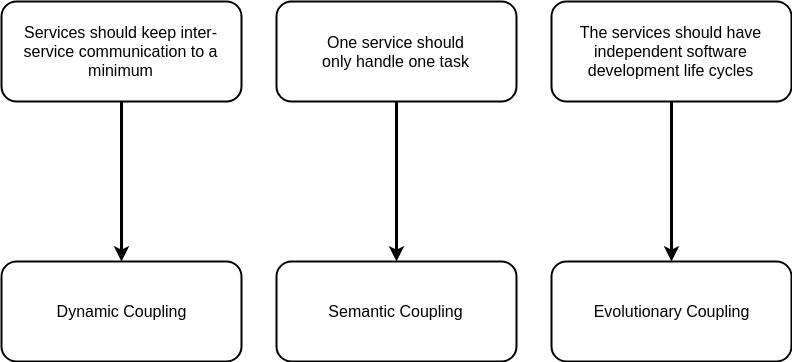
\includegraphics[width=.90\textwidth]{principles-of-microservices}
\caption{Mapping design principles of microservices to coupling types}
\caption*{\centering
  We detected that three of the most important design principles of the
  microservices paradigm map directly to three main types of coupling.
}
\label{fig:principles-of-microservices}
\end{figure}


\subsection{Dynamic coupling}

The term refers to any metric of coupling that measures how coupled
components are during their runtime, hence it is recorded during the execution
of a given application which ties it to \textit{dynamic program analysis}.

For instance, counting how often a certain component calls or accesses another
one is a metric described and covered in \ref{subsubsect:call-graph-dynamic}
as dynamic call graph generation based on \textit{execution counts}.
To clarify, a weighted and directed graph can be constructed when gathering
this \textit{dynamic coupling} metric for every single \textit{execution count}.
Hence, the weighted edges of the graph symbolize the \textit{execution counts}.

Finally, the first principle maps to this type of coupling due to the fact that
the \textit{dynamic coupling} information can be utilized to keep
communicative components from being spread over multiple microservices
(i.e. being clustered together), which would otherwise violate the first principle.


\subsection{Semantic coupling}

An undirected and weighted graph is constructed out of \textit{semantic coupling} information.
Precisely, it is measured how semantically similar two components are which
causes the weighted edge in the resulting graph that connects their vertices
to hold this similarity value.

Finally, the second principle maps to this type of coupling due to the fact that
the \textit{semantic coupling} information can be utilized to keep
components that cover a similar (or the same) task from being spread over
multiple microservices (i.e. being clustered together),
which would otherwise violate the second principle.


\subsection{Evolutionary coupling}

Again, an undirected and weighted graph can be constructed out of the
\textit{evolutionary coupling} information.
To be more precise, if two components change together more often it can be
inferred that their life cycles are more or less coupled.
To quantify this, the approach described in \ref{subsect:evolutionary-similarity}
is leveraged to precisely calculate how \textit{evolutionary coupled} components
are (i.e. how much their life cycles overlap) which is then represented
by the edge weights in the resulting weighted graph.

Finally, the third principle maps to this type of coupling due to the fact that
the \textit{evolutionary coupling} information can be utilized to keep
components that currently share the same software development life cycle
from being spread over multiple microservices (i.e. being clustered together),
which would otherwise violate the third principle.




\chapter{Extracting coupling information from software} \label{chap:extracting-coupling}

An important argument of our approach is that the coupling information
exhibited in chapter \ref{chap:rationale} are extracted out of the input
monolithic application automatically without any further user input.
In this chapter it is detailed which inputs need to be supplied and
how the three types of coupling are extracted out of them. Additionally,
a static program analysis is conducted as covered in this chapter.

Sometimes it is not possible to provide every of the four inputs which is why
at least the first and any two out of the three others have to be provided for our devised
methodology to still conduct its analysis correctly.

Finally, our methodology is focused on object-oriented programming,
hence we will from now on use the term \textit{class} instead of \textit{unit}
for describing the vertices of the constructed weighted graphs.
Moreover, the following descriptions are focused on Java applications,
however in chapter \ref{chap:implementation} we exhibit how other
languages and platforms can be added to the implementation.



\section{Static coupling extraction} \label{sect:static-coupling-extraction}

As discussed in more detail in chapter \ref{sect:software-as-weighted-graph},
we opt for also constructing a full static call graph which is covered
in subsection \ref{subsubsect:call-graph-static}.


\subsection{Walk\hyp based approach}

We utilize an approach that starts with the \code{main} method or methods of
the given application and then recursively walks down the classes and their
methods that are instantiated or invoked. Consequently, a graph with
possible cycles is constructed.
Both, class instantiations as well as method invocations can be registered
although as part of our methodology, both  will result in an edge connecting
the instantiating or invoking class vertex to the one it is instantiating
or invoking --- algorithm \ref{algo:class-walk} depicts this process.

\begin{algorithm}[ht]
\caption{Recursive walk trough classes and methods}
\label{algo:class-walk}
  \BlankLine
  \KwData{
    The source code or compiled code of an application
  }
  \KwResult{
    A graph with the classes as vertices and their instantiations and
    invocations toward others as the edges
  }
  \BlankLine
  $cg$ $\leftarrow$ empty list of pairs of classes representing the call graph\;
  $av$ $\leftarrow$ empty set for classes that have already been visited\;
  $cq$ $\leftarrow$ empty queue for classes that should be visited\;
  \BlankLine
  push the \code{main} methods of the application onto queue $cq$\;
  \BlankLine
  \While{class queue $cq$ is not empty}{
    $vc$ $\leftarrow$ pop class to visit next from queue $cq$\;
    \ForEach{method $vm$ of class $vc$}{
      \ForEach{class $ic$ instantiated or invoked from method $vm$}{
        add pair of $vc$ and $ic$ to call graph list $cg$\;
        \If{$ic$ is not in set of already visited classes $av$}{
          push class $ic$ onto class queue $cq$\;
          add class $ic$ to set of already visited classes $av$\;
        }
      }
    }
  }
  \BlankLine
  \Return{call graph list $cq$}\;
\end{algorithm}

For Java applications, both source code as well as compiled bytecode can
be utilized as the input to algorithm \ref{algo:class-walk}.
For both approaches, libraries exist that can access and iterate over
the classes and methods as detailed in chapter \ref{chap:implementation}.

The resulting static call graph is theoretically directed in the manner that it
gets constructed in algorithm \ref{algo:class-walk}, the first class in the class
pairs that are getting returned, is the vertex the edge is pointing away from.
Furthermore, it would be possible to count how often a class instantiates or
invokes another and accumulate this value as a weighted edge.
However, we opted to discard weights and to instead construct a directed, unweighted graph ---
although the directions are ignored in most cases as discussed in more detail in
section \ref{sect:implementation-database}.
The weights associated with a \textit{static coupling} graph
do not have much meaning since the range of the weights is not very significant
as certain business logic may instantiate a lot of other classes,
yet this does not strictly increase their coupling.
Specifically when compared to the other coupling types, potential edge weights
of the \textit{static coupling} graph are not very relevant, thus this graph
is plainly used for being able to obtain a final graph that covers the
entirety of the input monolithic application, as mentioned earlier.



\section{Dynamic coupling extraction} \label{sect:dynamic-coupling-extraction}

To extract the \textit{dynamic coupling} information, two general approaches
were detected and evaluated. Both have advantages and disadvantages which
are discussed in the following subsections. However, for both approaches,
the application has to be executed which involves a lot more overhead compared
to the previously exhibited \textit{static coupling} graph construction.

As part of our methodology, we decided that the user can choose which option
they want to use:
\begin{itemize}[noitemsep]
  \item The \textit{sampling\hyp based} approach has lower fidelity but
        also less impact on the runtime
  \item The \textit{instrumentation\hyp based} approach has high fidelity but
        also a large impact on the runtime
\end{itemize}
Our methodology works with both approaches with the difference that the results
with an \textit{instrumentation\hyp based} input are of better quality due to the
higher input fidelity. This is further detailed in the chapter on
\textit{\nameref{chap:implementation}}.


\subsection{Sampling\hyp based approach}

The first approach is more concerned with observing (i.e. monitoring)
the running application from the outside. The typical way to conduct this is
\textit{sampling\hyp based} application profiling. This means that with a preset
frequency, \(n\) times per second, a sample is recorded regarding what the
application is currently doing. This concerns actions such as
the memory usage, thread usage, which method is invoked how often, etc.

Focusing on the \textit{Java Virtual Machine} (JVM), as we target it with our
implementation, it ships with a built-in profiler,
called \textit{Java Flight Recorder} (JFR).
The JFR is a \textit{sampling\hyp based} profiler that is shipped
with \textit{OpenJDK} versions starting from 11 \cite{openjdk-jfr}.
For other platforms and languages, different profilers are available or built-in,
yet the idea to record profiling data at a certain sampling rate
stays the same, implementation details however differ from runtime to runtime.

The advantage of this approach is that the overhead on the runtime is kept to
a minimum. It is highly dependent on the implementation but in the example of
the JVM, the JFR only has a claimed overhead of about 1\% \cite{openjdk-jfr}.

The downside is that the fidelity of the recordings is highly dependent on the
sampling rate. The lower the sampling rate, the more likely it just misses
certain events (e.g. method invocations) which leads to the situation that
there is no certainty how much it actually recorded --- yet, this is true
for every \textit{sampling\hyp based} approach and an inherent problem of them.
However, the higher the sampling rate gets, the higher is the overhead for
recording gets, while still not eliminating said inherent problem.


\subsection{Instrumentation\hyp based approach}

Compared to the \textit{sampling\hyp based} approach described above,
an \textit{instrumentation\hyp based} approach can reach complete coverage of
theoretically every event happening during the runtime.
We are only concerned with method invocations, thus an
\textit{instrumentation\hyp based} approach in that case encompasses logging
every single method entry together with which method invoked it.

The disadvantage of this approach is that the impact on the runtime performance
is immense owing to the fact that every single method invocation is logged.

Generally, there are multiple ways to implement
\textit{instrumentation\hyp based} profiling, however the most common way
is some form of aspect-oriented programming (AOP) \cite{kiczales1997aop}.

The idea of AOP is to essentially inject extra functionality for
\textit{cross-cutting concerns}, which describe operations that are not
necessarily limited to a certain feature, such as logging \cite{kiczales1997aop}.
The idea itself is simple however, first the user defines \textit{cutting points},
which behave like patterns that are being matched on the source code,
for instance: \textit{at every method entry}.
They define where in the code base the extra functionality should be injected.
In the next step, the user defines source code that is then injected at every
\textit{cutting point} either in a static way at compile time or,
in the case of bytecode\hyp based languages, in the moment the bytecode is loaded
into the runtime environment \cite{kiczales1997aop}.
At runtime, at every \textit{cutting point}, method entries in our case,
the injected piece of logging code is executed just as the rest of the code
\cite{kiczales1997aop}.



\section{Semantic coupling extraction}

Similarly to the \textit{static coupling} again, the \textit{semantic coupling}
extraction only needs the source code itself. Importantly, human-readable,
not yet compiled source code is necessary as the semantics are lost in compiled
code since it does not contain natural language anymore.
We implemented an approach from scratch that conducts the steps regarding the
semantic similarity calculation from subsection \ref{subsect:semantic-similarity}:
\begin{enumerate}[noitemsep]
  \item Tokenization
  \item Stop word filtering
  \item Normalization
  \item Vectorization
  \item Relevance weighted via \textit{tf-idf}
  \item Latent semantic indexing (LSI)
\end{enumerate}
As detailed in subsection \ref{subsect:semantic-similarity},
specifically the first two steps are different when analyzing source code
compared to traditional natural language.


\subsection{Natural language processing on source code}

Just as the other input dimensions, we implemented our devised methodology
on the example of Java applications, hence this subsection will focus on
Java source code. Other rules would apply to other languages although
the general concept remains the same.

Regarding the first step, the \textit{tokenization}, an important difference to
the \textit{tokenization} of truly natural language is encountered.
Owing to the fact that line breaks are an important tool of syntactic separation
in programming, they are treated separately, this becomes apparent with an example.
Java source code as well as many other higher level programming languages have
the notion of recursive packages and importing them or parts of them into the
source code of other packages.
Consequently, source code such as the following example \ref{packages-and-imports}
would include package paths in the term list of the respective document
which would distort the result of the \textit{semantic coupling} analysis.
Thus, every line is parsed separately and language-specific keywords such as
\code{package} or \code{import} trigger that the line gets discarded.

\begin{lstlisting}[caption=Packages and imports in Java, label=packages-and-imports, language=Java, breaklines=true]
package codes.jakob.semanticcoupling.parsing

import codes.jakob.semanticcoupling.model.Document
import codes.jakob.semanticcoupling.model.NaturalLanguage
import codes.jakob.semanticcoupling.model.ProgrammingLanguage
import codes.jakob.semanticcoupling.model.Term
import codes.jakob.semanticcoupling.normalization.Lemmatizer
import codes.jakob.semanticcoupling.normalization.Normalizer
import codes.jakob.semanticcoupling.normalization.Stemmer
\end{lstlisting}

Next, every line of the source code is stripped of non\hyp word characters
(i.e. \code{W} from regular expressions) which is every character
but a-z, A-Z, 0-9, and the underscore character \cite{ieee1992posix}.
Before that step, explicit strings (i.e. text in double quotes) are separately
saved so they do not lose their meaning when stripping the double quotes.
Additionally, the explicit strings as well as every other text that is still
left then and matches a camel-case pattern is split into a new term at every
\textit{camel hump}. Moreover, numeric characters as well as single characters
are filtered out, as both provide no relevant semantic meaning.

Furthermore, as part of the second step, the \textit{stop word filtering},
a list with stop words specific to the Java language is used to filter out
terms that are contained in the list. The list was crafted by us in line with
the official Java language specification \cite{oracle-java11}.
Examples for terms that are classified as stop words include:
\begin{itemize}[noitemsep]
  \item \code{class}
  \item \code{public}
  \item \code{static}
  \item \code{void}
\end{itemize}

Finally, everything that was not filtered out until this point is split
at white space characters (i.e. \code{t} from regular expressions)
\cite{ieee1992posix}.
Additionally, every resulting term is converted to lower case so that
the subsequent steps handle the same term in different cases as
semantically indifferent.

The remaining steps are conducted just as described in subsection
\ref{subsect:semantic-similarity} since after the second step,
the following steps work on term lists as part of documents of the corpus
\(t_i \in d_i, d_i \in C\), which, at that point, are containing regular natural language.



\section{Evolutionary coupling extraction} \label{sect:evolutionary-coupling-extraction}

The last input dimension, the \textit{evolutionary coupling}, needs different
input. Instead of the application code itself, a log file generated by the
utilized version control system (VCS) is required.
This mandates that a VCS is used during the development of the input application.


\subsection{Mining version control system data}

The approach leveraged to mine VCS data is modeled after the methodology of
Tornhill \cite{tornhill2015crimescene} which is exhibited in subsection
\ref{subsect:evolutionary-similarity}.

Theoretically, every VCS that has the notion of revisions that include files
and that is able to generate a log file which details past revisions together
with the files involved, can be used to extract \textit{evolutionary coupling}
information. Common VCS that we also support as part of our implemented
methodology detailed in chapter \ref{chap:implementation} are:
\begin{itemize}[noitemsep]
  \item \textit{Git}
  \item \textit{Subversion}
  \item \textit{Mercurial}
  \item \textit{Perforce}
  \item \textit{Team Foundation Server}
\end{itemize}
All of the above also support to only generate a partial log for a certain
time period. However, \textit{Perforce} and \textit{Team Foundation Server}
only support to log the last \(n\) revisions compared to a time\hyp based range
\cite{perforce, team-foundation-server}.

A caveat with this approach is that by default, the log files will only
include files. Owing to the fact that in applications written in Java,
one file is also equivalent to one class, we can generate the coupling graph
without any changes to the log format. Nevertheless, it would be possible
to extend the \textit{evolutionary coupling} information extraction to support
languages that might keep multiple \textit{units} (i.e. the vertices in the graph)
in the same file by generating more detailed log files on a line level within
the files. However, this is not covered by our work as we focus on
Java applications for our initial implementation.

After parsing the input log file, differing based on the utilized VCS,
the process described in subsection \ref{subsect:evolutionary-similarity}
generates the weighted \textit{evolutionary coupling} graph with the same
structure as the other ones such that the vertices \(v_i \in V\) are the classes
extracted from the VCS log file while the edges \(e_i \in E\) are resembling
that two classes have overlapping software development life cycles.
The weight of the edges is a percentage that indicates how much the
life cycles overlap \(W(e_i) \in [0.0, 1.0]\).

Finally, as discussed in subsection \ref{subsect:evolutionary-similarity},
we use a threshold for this extraction step to filter out noise.
The values are constants that can be changed while the defaults that we employ are:
\begin{itemize}[noitemsep]
  \item Minimum shared revisions between entities: 1
  \item Time period \([t_1, t_2]\): Every day from \([00:00, \ 23:59]\)
\end{itemize}
For clarification, figure \ref{fig:vcs-log-timeline} depicts an example
timeline to show how the \textit{evolutionary coupling} is calculated
via a given VCS log while the direction of the coupling relationship is taken
that was extracted out of the static analysis into a directed graph.

\begin{figure}[htbp]
\centering
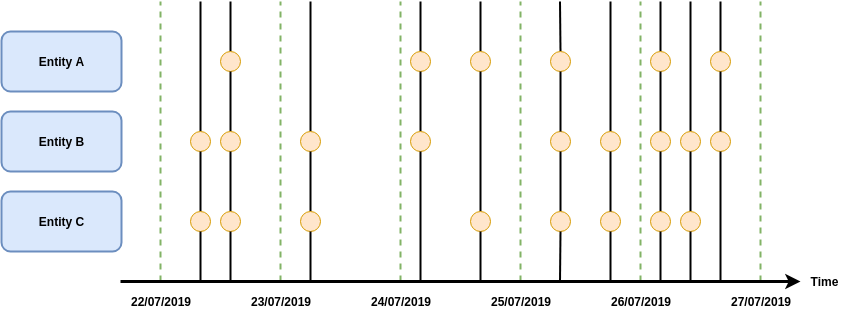
\includegraphics[width=.96\textwidth]{vcs-log-timeline}
\caption{An example timeline of a VCS log}
\caption*{\centering
  A textual VCS log is mined for \textit{evolutionary coupling} information
  by analyzing how many percent of the shared revisions of two entities
  do overlap. The figure specifically depicts the usage of time ranges
  and thresholds to obtain sound data.
  The solid lines are depicting revisions.
  The dotted lines are depicting midnight in between two days on the timeline.
  In the example, according to our explanation in
  \ref{sect:evolutionary-coupling-extraction}, the \textit{evolutionary coupling}
  values would be as follows (the values are rounded down):
  \begin{center}
  \begin{tabular}{|c|c|c|c|}\hline
    \backslashbox{To}{From}
    ~   & A     & B     & C     \\\hline
    A   & --    & 0.55  & 0.50  \\\hline
    B   & 0.83  & --    & 0.87  \\\hline
    C   & 0.66  & 0.77  & --    \\\hline
  \end{tabular}
  \end{center}
}
\label{fig:vcs-log-timeline}
\end{figure}




\chapter{Creating microservice recommendations} \label{chap:creating-service-recommendations}

\section{Representing software as weighted graphs} \label{sect:software-as-weighted-graph}

Our methodology works by clustering a weighted graph hence we need to construct
it first. As discussed in chapter \ref{chap:rationale}, three general
coupling types were chosen to be leveraged for devising the microservice
candidates recommendations.
Precisely, the input monolithic application gets analyzed from the view of
each of these coupling types, called dimensions from now on.

Out of each of the input dimensions, a weighted graph is constructed with the classes
as the vertices \(v_i \in V\) and the coupling values between the classes
as the weighted edges \(e_i \in E\) representing a percentage
\(W(e_i) \in [0.0, 1.0]\) --- resulting in a weighted graph \(G = (V, E)\).
Consequently, we receive three separate weighted graphs with the different
input dimensions as the edge weights.

However, the other extraction methods (i.e. dimensions) covered in the
sections below entail one problem that would would discredit
our whole methodology --- they oftentimes do not cover the entirety of the
input monolithic application in regard to featuring every class of it
as vertices in the resulting weighted graph.
As a consequence, it is possible that all three weighted graphs constructed
out of the three coupling types are not complete in the sense that they cover
the entirety of the input application. As this would defeat the purpose of
our approach, an additional static call graph is constructed to be certain
that the final graph covers the whole application.



\section{Merging input dimensional graphs} \label{sect:merging-graphs}

Finally, four graphs are constructed out of the four input dimensions
that need to be merged into a combined one so that it can be clustered eventually.
Essentially, this encompasses a two step process with the first being
a set-theoretic union of the two first graph tuples \(G_i = (V, E)\) such that:
\[
  G_{combined} = G_{static} \cup G_{dynamic}
\]
Importantly, this step utilizes a union owing to the fact
that the first two input dimensions have downsides in producing a graph
that covers the whole application.
Nevertheless, they complement each other since they cover separate important
aspects of detecting the distinct types of coupling.

Static program analysis has the shortcoming that certain aspects of a written
application are only known at runtime such as the usage of
\textit{reflection} \cite{landman2017reflection}.
On the other hand, dynamic program analysis entails the problem that
it is by no means guaranteed that every class of the executed application
is called or even instantiated --- the resulting graph is highly dependent
on the workload during the dynamic analysis.

In the second step, the two remaining input dimensional graphs are merged into
the combined graph \(G_{combined}\):
\[
  G_{combined} = G_{combined} \cap G_{semantic} \cap G_{evolutionary}
\]
As part of this step, set-theoretic intersections are used instead as the
combined graph resulting out of the merger of the static and the dynamic
program analysis acts as a single source of truth --- classes that are not
connected in there are not able to instantiate or invoke each other in the
given application hence intersections are utilized to keep this single source
of truth.
Specifically regarding the \textit{semantic coupling} graph, the semantic
similarity can be calculated for any two given classes regardless of their
connection in the input application code base.

Consequently, unions ensure that the entirety of the given
monolithic application is covered as part of the graph-theoretic representation
while intersections add more information to the existing combined graph.
Precisely, all vertices from the first two graphs are added to the combined one:
\[
  V_{combined} = V_{static} \cup V_{dynamic}
\]
For the edges, the merging is twofold. The edges themselves are only getting
sourced from the first two input graphs to connect the vertices \(V_{combined}\)
while the other two input graphs do not add new edges but just enrich the
information of existing ones:
\[
  E_{combined} = E_{static} \cup E_{dynamic} \cap E_{semantic} \cap E_{evolutionary}
\]
However, the edge weights should not just be added up as all of them resemble
percentages. Instead, we use a modifiable \textit{edge weighting formula} which
is defining factors for each input dimension to increase or decrease its importance
in calculating the combined weight of each edge \(\forall e_i \in E_{combined}\)
in the combined graph \(G_{combined}\). Owing to the fact, that the
\textit{static coupling} dimension does not yield edge weights as covered in
section \ref{sect:static-coupling-extraction}, it is excluded from
the \textit{edge weighting formula}:
\small
\begin{equation*}
\begin{split}
  W_{combined}(wf_{dynamic}, wf_{semantic}, wf_{evolutionary}) = \\
  \frac{
    wf_{dynamic} \times W(e_{dynamic}) +
    wf_{semantic} \times W(e_{semantic}) +
    wf_{evolutionary} \times W(e_{evolutionary})
  }{
    wf_{dynamic} +
    wf_{semantic} +
    wf_{evolutionary}
  }
\end{split}
\end{equation*}
\normalsize
In the above formula, the weight factors \(w_x\) can then be substituted
with custom factors. Our default setting is an average with all the
weight factors being \(1\).
\newline
Once the combined graph \(G_{combined}\) has been constructed, the next step is
to apply graph clustering to it such that groups of vertices that have strong
coupling, resembled by the combined edge weights
\(W_{combined}(wf_{dynamic}, wf_{semantic}, wf_{evolutionary})\) in between them,
are more likely to end up in the same cluster.
These clusters would then mirror the notion of the \textit{bounded contexts},
introduced in subsection \ref{subsect:ms-principle-2}.
Thus, each cluster then resembles one microservice candidate recommendation.

Consequently, the question arises which approach to take in clustering the
constructed graph \(G_{combined}\) at hand, respectively which graph clustering
algorithm to choose, to devise the recommendations as optimally as possible.



\section{Survey of graph clustering algorithms} \label{sect:graph-clustering-algorithm-survey}

The idea of graph clustering was exhibited in the \textit{\nameref{chap:background}}
chapter together with a range of available, renowned algorithms.
A variety of graph clustering algorithms exists with a variety of different
goals, mechanisms, and features
\cite{lancichinetti2009community, fortunato2010community, danon2005comparing}.
Consequently, a dozen renowned graph clustering algorithms out of the above sources
were evaluated and assessed regarding their usability for our work.
A total of nine renowned graph clustering algorithms were chosen and classified
in table \ref{table:graph-clustering-survey}, the others had no available
reference implementation.
The way that classifications are negated was chosen so that $\oplus$
is a positive feature regarding the utilization as part of our work.

Eventually, apart from the \textit{Girvan-Newman} algorithm, the first seven
respectively seven algorithms from table
\ref{table:graph-clustering-survey} were selected to be utilized as part of our work.
We chose to not select \textit{Girvan-Newman} as well despite its positive evaluation as Newman
designed an improved version of it shortly after together with Clauset and Moore
\cite{clauset2004modularity}.
The other two remaining algorithms had severe downsides that made them unsuable
as part of our methodology (i.e. not offering a hard clustering respectively
not working on weighted graphs).
The selected graph clustering algorithms are discussed in more detail in the
\textit{\nameref{chap:background}} subsection regarding
\textit{\nameref{subsect:renowned-graph-clustering-algorithms}}.
The citation numbers in the table are also referenced there.

\begin{table}[ht!]
\def\arraystretch{1.60}
\begin{tabularx}{\textwidth}{|Y||p{2.5cm}|Y|Y|Y|Y|Y|Y|Y|Y|Y|}
 \hline
 \rot{Citations~} & \rot{Runtime complexity~} & \rot{Implementation available~} & \rot{Does not require amount of clusters~} & \rot{Deterministic~} & \rot{Considers weighted edges~} & \rot{Hard clustering~} & \rot{Hierarchical~} \\
 \hline\hline
 \cite{girvan2002community}     & \(\mathcal{O}(n^3)\)          & $\oplus$  & $\ominus$  & $\oplus$   & $\oplus$  & $\oplus$  & $\oplus$ \\\hline
 \cite{vandongen2000graph}      & \(\mathcal{O}(nk^2)\)         & $\oplus$  & $\oplus$   & $\oplus$   & $\oplus$  & $\oplus$  & $\ominus$ \\\hline
 \cite{pons2005computing}       & \(\mathcal{O}(mn)\)           & $\oplus$  & $\ominus$  & $\oplus$   & $\oplus$  & $\ominus$ & $\ominus$ \\\hline
 \cite{clauset2004modularity}   & \(\mathcal{O}(md \log{n})\)   & $\oplus$  & $\oplus$   & $\oplus$   & $\oplus$  & $\oplus$  & $\oplus$ \\\hline
 \cite{blondel2008modularity}   & \(\mathcal{O}(n)\)            & $\oplus$  & $\oplus$   & $\oplus$   & $\oplus$  & $\oplus$  & $\oplus$ \\\hline
 \cite{raghavan2007lpa}   & \(\mathcal{O}(n)\)                  & $\oplus$  & $\oplus$   & $\ominus$   & $\oplus$  & $\oplus$  & $\ominus$ \\\hline
 \cite{rosvall2008infomap}      & \(\mathcal{O}(n)\)            & $\oplus$  & $\oplus$   & $\ominus$  & $\oplus$  & $\oplus$  & $\oplus$ \\\hline
 \cite{biemann2006chinese}      & \(\mathcal{O}(n)\)            & $\oplus$  & $\oplus$   & $\ominus$  & $\oplus$  & $\oplus$  & $\ominus$ \\\hline
 \cite{reichardt2004detecting}  & \(\mathcal{O}(n)\)            & $\oplus$  & $\ominus$  & $\ominus$  & $\oplus$  & $\ominus$ & $\ominus$ \\\hline
 \cite{donetti2004detecting}    & N/A                           & $\oplus$  & $\ominus$  & N/A        & $\ominus$  & $\oplus$  & $\oplus$ \\\hline
\end{tabularx}
\caption{Graph clustering algorithm survey matrix}
\caption*{\centering
  All of the information necessary for the classification including the
  runtime complexity indications are taken out of the original papers of the
  authors which leads to the fact that some information is unknown as
  the authors did not calculate or disclose this information.
  The signs that are used in the matrix correspond to the following meaning:
  \begin{itemize}[noitemsep]
    \item $\oplus$: The statement of the respective cell is \textit{true}
    \item $\ominus$: The statement of the respective cell is \textit{false}
    \item N/A: The statement of the respective cell is \textit{not available}
  \end{itemize}
  The way that classifications are negated was chosen so that $\oplus$
  is a positive feature regarding the utilization as part of our work.
%   The citation numbers stand for the following algorithms:
%   \begin{itemize}[noitemsep]
%   \item \cite{girvan2002community}: Girvan-Newman
%   \item \cite{vandongen2000graph}: MCL
%   \item \cite{pons2005computing}: Walktrap
%   \item \cite{clauset2004modularity}: Clauset-Newman-Moore
%   \item \cite{blondel2008modularity}: Louvain
%   \item \cite{raghavan2007lpa}: Label Propagation
%   \item \cite{rosvall2008infomap}: Infomap
%   \item \cite{biemann2006chinese}: Chinese Whispers
%   \item \cite{reichardt2004detecting}: Spinglass
%   \item \cite{donetti2004detecting}: Commfind
%   \end{itemize}
}
\label{table:graph-clustering-survey}
\end{table}

The characteristics chosen for the survey are discussed in the following paragraphs.

\paragraph{Runtime complexity}
The runtime complexity of a graph clustering algorithm is not overly
important for our methodology and definitely does not eliminate a given algorithm,
nevertheless, it is interesting to include this metric in the conducted survey.

\paragraph{Implementation available}
This characteristic is the first rated one as it is the most important for our
methodology in the sense that the utilization of an algorithm as part of
the implementation of our methodology is only possible when an implementation
of that algorithm is available.

\paragraph{Does not require amount of clusters} \label{graph-clustering-algorithm-survey-amount-of-clusters}
For our devised methodology, it is beneficial if the utilized graph clustering
algorithm does not require a desired amount of clusters a priori owing to
the fact that this number can only be estimated at best by a software engineer
using our implementation.
Nevertheless, some algorithms, and more importantly even some of the selected ones,
require said amount of clusters as an input parameter.
To circumvent this problem we came up with the solution to execute the affected
algorithms multiple times with the same input and differing cluster amounts
for a fixed number of iterations. Afterwards, the run that produced the highest
scoring metric is selected in place where other algorithms that are not affected
would have yielded only one output in the first place.
This may sound like a very ineffective solution but due to the fact that
a single run of any graph clustering algorithm is completely isolated from
another one, this process can be executed concurrently with ease.
How exactly this is implemented is discussed in chapter \ref{chap:implementation}.

\paragraph{Deterministic}
A non\hyp deterministic graph clustering algorithm might produce different
results over the course of multiple executions. This effect is not a desired
characteristic regarding our devised methodology but it can be mitigated
with the solution discussed in the previous paragraph again.

\paragraph{Considers weighted edges}
This characteristic is of great importance for us since the input graphs
will always be weighted. Furthermore, the whole idea of our methodology
is to cluster similar vertices where the similarity is resembled via edge weights.

\paragraph{Hard clustering}
The term \textit{hard clustering} describes that the output clustering
of a given graph clustering algorithm assigns one and only one cluster
to each vertex of the graph. Comparatively, \textit{soft clustering} or
\textit{fuzzy clustering} can assign a vertex to multiple clusters which
produces overlapping clusters \cite{lancichinetti2009community}.
Similarly to the previous characteristic, this is not desired regarding our
devised methodology as every vertex can only belong to one microservice
which requires \textit{hard clustering} (i.e. partitioning).

\paragraph{Hierarchical}
The last characteristic is not directly important for our methodology
as we are only interested in the final output of the clusters as partitions.
Nevertheless, as discussed in section \ref{sect:future-work},
this property of graph clustering algorithms could be leveraged for future features.
\newline

The reason that the first seven from table \ref{table:graph-clustering-survey}
were selected is that specifically the characteristics
\textit{Considers weighted edges} and \textit{Hard clustering} are mandatory
for our devised methodology to function.



\section{Clustering the combined weighted graph}

Regardless of which of the first nine graph clustering algorithms out of
table \ref{table:graph-clustering-survey} is chosen, the input and output
are the same at their core.
Although the exact input and output formats differ between the algorithms,
it always boils down to passing a list of edges to the algorithm ---
listing \ref{graph-clustering-algorithm-input} depicts this kind of input format.
In this example input, the format follows a tuple of three items (i.e. a triple),
namely a vertex, another vertex it is connected to, and the edge weight of the
edge connecting them:
\[
  I_i = (v_1, \ v_2, \ W(e_{(1,2)}))
\]
such that \(v_1, v_2 \in V, \ e_{(1,2)} \in E, \ G = (V, \ E)\) while
\(e_{(1,2)}\) is the edge connecting the vertices \(v_1\) and \(v_2\).

\begin{lstlisting}[caption=Example graph clustering algorithm input, label=graph-clustering-algorithm-input, breaklines=true]
1 2 0.50
4 5 0.11
5 6 0.55
6 5 0.60
3 2 0.19
\end{lstlisting}

In this format, the entire input graph is serialized while each line resembles
a single edge. The integers used for the vertices are their identifiers,
some algorithms require identifiers from \([1, n] \in \mathbb{Z}\) where \(n\)
is the number of edges, others also work with arbitrary strings as identifiers.
This fact is discussed in more detail in chapter \ref{chap:implementation}.

As mentioned in section \ref{sect:background-graph-clustering}, many graph
clustering algorithms discard directions in the input graph which is no problem
for our methodology as the resulting microservice candidate recommendations
are finally unidirectional in any case.

After serializing the input graph, the chosen algorithm clusters the graph
and returns the clustering as its output. The inner workings of the chosen
algorithm are assumed as a black-box function at this point since this was
already discussed in subsection \ref{subsect:renowned-graph-clustering-algorithms}
and as it is not important for the understanding of this section.

Similarly to the input, the output of the selected algorithms also shares
a common notion regarding the format. This example output format is depicted
in listing \ref{graph-clustering-algorithm-output}.
In contrast to the input format, the output contains vertices compared to edges
and the cluster identifier of each vertex compared to edge weights,
as pairs this time:
\[
  O_i = (v_i, \ c_i)
\]
such that \(v_i \in V, \ G = (V, \ E)\) while \(c_i \in C\) resembles the
cluster that was assigned to the respective vertex by the graph clustering
algorithm. The cluster identifiers commonly range from \([1, n] \in \mathbb{Z}\)
where \(n\) is the amount of clusters. Moreover, they can be duplicated
which signifies that vertices were put into the same cluster.

\begin{lstlisting}[caption=Example graph clustering algorithm output, label=graph-clustering-algorithm-output, breaklines=true]
1 1
2 1
3 1
4 2
5 3
6 3
\end{lstlisting}

Finally, we deserialize the output into a Java object so it can be used to
calculate metrics and render the clustered weighted graph for the user.




\chapter{Calculating metrics on microservice recommendations} \label{chap:metrics}

As laid out in chapter \ref{chap:rationale}, we aimed for an objective
mapping of the input monolithic application to its graph-theoretic representation
and the clustered output respectively.
Thus, it was important to us to also devise objective metrics, numeric in nature,
to be able to evaluate the results of our methodology and to answer \textit{RQ2}.

In total, we devised a total of 17 metrics that can be sorted into three sets ---
some of them being more general and overarching while others are more specific
to the problem at hand by offering a direct order of magnitude regarding the
quality of the produced output. The three sets of metrics are covered
in the following sections while the devised metrics are the following:
\begin{itemize}
  \item Dynamic analysis input fidelity
  \item Semantic analysis input fidelity
  \item Evolutionary analysis input fidelity
  \item Amount of clusters
  \item Amount of inter-cluster edges
  \item Ratio of inter-cluster edge weight
  \item Mean cluster size
  \item Dynamic Mean Cluster Factor
  \item Semantic Mean Cluster Factor
  \item Evolutionary Mean Cluster Factor
  \item Average Mean Cluster Factor
  \item Total Mean Cluster Factor
  \item Dynamic Coupling Modularity
  \item Semantic Coupling Modularity
  \item Evolutionary Coupling Modularity
  \item Average Coupling Modularity
  \item Total Coupling Modularity
\end{itemize}



\section{Input fidelity} \label{sect:input-fidelity-metrics}

The first set of metrics is not directly answering \textit{RQ2} but is interesting
to look at nevertheless as the \textit{input fidelity} bears implications
regarding the eventual quality of the clustering.
The term \textit{input fidelity}, that we devised, describes how many percent
of the classes of the entire application a given input covers which gives us
three different \textit{input fidelity} metrics:
\begin{itemize}[noitemsep]
  \item Dynamic analysis input fidelity
  \item Semantic analysis input fidelity
  \item Evolutionary analysis input fidelity
\end{itemize}

Precisely, this measures how many percent of the edges of a certain input graph
are also part of the combined graph \(G_{combined}\) covered in chapter
\ref{sect:software-as-weighted-graph}:
\[
  IF(G_{input}, G_{combined}) = \frac{\vert E(G_{input}) \vert}{\vert E(G_{combined}) \vert}
\]
The higher this percentage is, the better as it increases the confidence
that the results are actually resembling the quality that was calculated for them.
Comparatively, if all of the inputs have low \textit{input fidelities},
our methodology still produces output but the confidence that it is any good is low.

There is no threshold of the \textit{input fidelity} being too low,
we instead devised it as a supporting measurement to corroborate the outputs
of our methodology. All three of the input dimensions have different
considerations in regard to achieving a high \textit{input fidelity} value.

\paragraph{Dynamic coupling}
The \textit{dynamic coupling} has the main problem that the \textit{input fidelity}
is highly dependent on the workload that was executed during runtime when the
dynamic program analysis was conducted. Ideally, every edge of the combined graph
should also be part of the \textit{dynamic coupling} graph as it can be
theoretically executed, however in reality this is not often the case.
Specifically when utilizing a \textit{sampling\hyp based} profiler,
as discussed in section \ref{sect:dynamic-coupling-extraction},
the likelihood of reaching \(100\%\) \textit{input fidelity} is very low ---
and even with an \textit{instrumentation\hyp based} profiler,
every single possible branch of the program at hand actually needs to be
executed during the recording which is unlikely with non\hyp synthetic workloads
which are preferred since the generated microservice candidate recommendations
should not be based on synthetic workloads as they would skew the results.

\paragraph{Semantic coupling}
On the other hand, the \textit{semantic coupling} graphs should reach an
\textit{input fidelity} of \(100\%\) since a percentage of how semantically
similar two classes in a code base are can always be calculated,
even if they are not similar at all, \(0\%\) similarity will still
count toward the \textit{input fidelity}.

\paragraph{Evolutionary coupling}
Similarly to the \textit{dynamic coupling}, the \textit{evolutionary coupling}
graphs are nearly never reaching full \textit{input fidelity}.
The \textit{evolutionary coupling} graph is affected by the threshold used
to filter out noise that was introduced in subsection \ref{subsect:evolutionary-similarity}.
These thresholds will lead to certain edges not being part of the
\textit{evolutionary coupling} graph which will lower the \textit{input fidelity}
as a result.



\section{General clustering quality}

The second set of metrics now answers \textit{RQ2} but was given its own set
owing to the fact that for all four metrics in this set it can not be strictly
defined if low value are better or worse. This reason becomes apparent when
looking at the actual metrics:
\begin{itemize}[noitemsep]
  \item Amount of clusters
  \item Amount of inter-cluster edges
  \item Ratio of inter-cluster edge weight
  \item Mean cluster size
\end{itemize}

\paragraph{Amount of clusters}
For instance, for the first one in this set it cannot be said that lower or
higher values are better or worse. With the \textit{amount of clusters},
\(\vert C \vert\) one wants a value in the middle without knowing where
the middle exactly lies --- more clusters convert to more microservice
candidate recommendations which is not necessarily better.
Nevertheless, in this case the metric offers an important insight regarding
the question of granularity of the produced output.

\paragraph{Amount of inter-cluster edges}
This metric is calculated by counting the amount of edges in the combined graph
\(G_{combined}\) that are in between vertices that do not belong to the same cluster:
\[
  \vert E_{inter}(G_{combined}) \vert =
  \vert \{ e_i(v_j, \ v_k) \in E(G_{combined}) \mid C(v_j) \neq C(v_k) \} \vert
\]
Hence, this metric is a combination of the \textit{Afferent Coupling} and
\textit{Efferent Coupling} metrics by Martin \cite{martin2000design}.
The smaller this value is the less external interfaces the microservice candidate
recommendations will have thus it is generally preferred for this metric to be
low however it is not desirable to achieve the lowest as possible as this
might sacrifice other metrics such as the \textit{Coupling Modularity}.

\paragraph{Ratio of inter-cluster edge weight}
Similarly to the previous metric, this metric measures how many percent
of the total accumulated edge weight lies in between clusters:
\[
  RW_{inter}(G_{combined}) =
  \frac{
    \sum_{e_j \in E_{inter}(G_{combined})}^{\vert E_{inter}(G_{combined}) \vert} W(e_j)
  }{
    \sum_{e_k \in E(G_{combined})}^{\vert E(G_{combined}) \vert} W(e_k)
  }
\]
The rationale here is the same as for the \textit{amount of inter-cluster edges}.

\paragraph{Mean cluster size}
Regarding the last metric of the second set, it is important to know that
as part of the implementation of our methodology detailed in chapter
\ref{chap:implementation}, the size in bytes is calculated for every class
of the input monolithic application during the initial analysis step.
In the case of Java applications, the compiled JVM byte-code is used for this
calculation as it is more standardized and misses arbitrary characters such as
line breaks. For other languages or platforms, the source code might be a
feasible option after being normalized (e.g. stripped off line breaks).
Thus, a way to calculate the accumulated size of a cluster is required beforehand:
\[
  S(c) = \sum_{v_i \in V(c)}^{\vert V(c) \vert} S(v_i)
\]
Finally, this metric calculates the population mean size over all of the
generated clusters:
\[
  \mu_{S(C)} = \mu(\{ c_i \in C \mid S(c_i) \})
\]
This gives an insight regarding the size of the clustering which, similarly to
the \textit{amount of clusters} metric, depicts the notion of granularity.



\section{Modularity metrics}

Finally, the third set of devised metrics is the most interesting one since,
compared to the second set, it not only answers \textit{RQ2} but also directly
measures the quality of the resulting clustering.
In contrast to the second set, for the third set is always holds true that
higher values are better.

There are no metrics directly measuring the modularity of a microservice
decomposition. Thus, we looked into related domains and found a certain paper
over and over again in the reference lists of others
\cite{maqbool2007hierarchical, praditwong2010software, tsantalis2009identification,  jiang2006visualizing}:
The \textit{Modularization Quality} (MQ) metric was devised by Mitchell and Mancoridis
\cite{mitchell2006automatic} in a paper that researched a very similar idea to ours ---
instead of clustering classes to achieve a microservice decomposition, they cluster
classes of a given application to construct a top\hyp level package structure for it.
Additionally, Mitchell and Mancoridis validated their metric in their work
\cite{mitchell2006automatic}.
Consequently, this metric is perfectly suited for our methodology as its goal is aligned with ours:
\begin{displayquote}
\emph{"MQ determines the quality of a partition quantitatively as the trade-off
between interconnectivity (i.e., dependencies between the modules of two distinct
subsystems) and intraconnectivity (i.e., dependencies between the modules of
the same subsystem). This trade-off is based on the assumption that well-designed
software systems are organized into cohesive subsystems that are loosely interconnected.
Hence, MQ is designed to reward the creation of highly cohesive clusters that
are not coupled excessively."}~\cite{mitchell2006automatic}
\end{displayquote}

The first step is to calculate \textit{Cluster Factor} (CF) values for every cluster
that range on a scale of \([0.0, 1.0]\), as explained in section
\ref{sect:background-graph-clustering}.
As the last step of calculating the \textit{Modularization Quality} metric,
the original paper claims to sum up the \textit{Cluster Factor}
values of every cluster while this makes no sense when comparing the performance
of different graph clustering algorithms as the metric generally grows with
rising amounts of clusters hence favoring algorithms that produce higher cluster
amounts. Consequently, we decided to instead take the arithmetic mean of all of
the \textit{Cluster Factor} values while the ones that yield $\infty$ due to
division\hyp by\hyp zero are treated as $0.0$ as the original paper did as well
\cite{mitchell2006automatic}. In this way, the final metric value
ranges on the scale of \([0.0, 1.0]\) again instead of having no scale.
We propose the name \textit{Mean Cluster Factor} (mCF) for this metric.

Thus, as this set of metrics consists of ten metrics based on the and
\textit{Mean Cluster Factor} and \textit{Modularity} metrics, introduced in
section \ref{sect:background-graph-clustering}:
\begin{itemize}[noitemsep]
  \item Dynamic Mean Cluster Factor
  \item Semantic Mean Cluster Factor
  \item Evolutionary Mean Cluster Factor
  \item Average Mean Cluster Factor
  \item Total Mean Cluster Factor
  \item Dynamic Coupling Modularity
  \item Semantic Coupling Modularity
  \item Evolutionary Coupling Modularity
  \item Average Coupling Modularity
  \item Total Coupling Modularity
\end{itemize}
The \textit{Modularity} metrics are included but not preferred since some
of our supported graph clustering algorithms use it as their fitness function
which causes the metric to favor them. Nevertheless, both kinds of metrics
are specifially interesting when combined as high scores in both are a sign of
a good partition and graph clustering algorithm in general.
Precisely, the first three of each kind of the above share the same underlying
equation of calculating the \textit{Mean Cluster Factor} or \textit{Modularity}
of their respective coupling graph (e.g. \(G_{semantic}\)).
The \textit{Average Mean Cluster Factor} and the \textit{Average Coupling Modularity}
are the arithmetic means of the set of the first three metrics of their kind.
Lastly, the \textit{Total Mean Cluster Factor} and \textit{Total Coupling Modularity}
are the calculations performed on the combined graph \(G_{combined}\).

Specifically this last set is directly answering \textit{RQ2} by offering
numeric and objective metrics that can directly be translated into how
qualitative the generated microservice candidate recommendations are.




\chapter{Implementation} \label{chap:implementation}

In the last chapters, we described the methodology that we devised to answer
\textit{RQ1} as well as the metrics we created to answer \textit{RQ2} ---
both of these were so far theoretic in nature.
However, since the subject of our work is very applied and close to industry
in practice, on top of the theoretic description, we additionally designed
and build a fully-functional implementation of our devised methodology.

Our implementation carries the name \textit{Steinmetz} which is the German
word for \textit{stonemason}. The name was chosen as our application is used
to cut one large stone, the monolith, into many smaller stones, the microservices.
Additionally, we published our implementation as open source software,
licensed under the \textit{Apache License v2}
\footnote{\url{https://github.com/loehnertz/Steinmetz/blob/develop/LICENSE}} ---
the entire source code can be found on GitHub
\footnote{\url{https://github.com/loehnertz/Steinmetz/}}.

The three parts of the application are all bundled into \textit{Docker} containers
via \textit{Docker Compose} which allows for easy boot-up and tear-down without
installing any dependencies on the operation system apart from \textit{Docker}
and \textit{Docker Compose} themselves \cite{docker} \cite{docker-compose} ---
a big advantage when putting our implementation to use.



\section{Architecture}
The general, high-level architecture of our application is a three-tier
web-based design. The three tiers are namely the front-end, the back-end,
as well as the database.

The front-end is built as a \textit{single page application} (SPA),
running in a web browser. It is just consisting of static HTML, CSS, and JS files
that are purely being interpreted and executed by the web browser.

The back-end is written in Kotlin, runs as a server process, and exposes
a REST-API that the front-end will use and consume to upload and fetch information.

The database is persisting data that needs to be available even when the
back-end shuts down and starts again. However, in our application,
the purpose of the database is mainly that to cache data after it has
been initially processed, as this needs some time. The data itself can be
rebuilt with the same input deterministically and will be rarely modified.

As pointed out, for smaller scale applications, a monolithic architecture
makes sense more often by being easier to implement and maintain.
Thus, we designed the back-end of our application in a monolith manner.

The implemented application has two major functionalities that can be used
via RESTful endpoints which are detailed in section \ref{sect:implementation-back-end}
and depicted in figure \ref{fig:architecture-overview}.
These functionalities are to analyze and persist an input monolithic application
as well as clustering and retrieving it again as a separate step.

\begin{figure}[htbp]
\centering
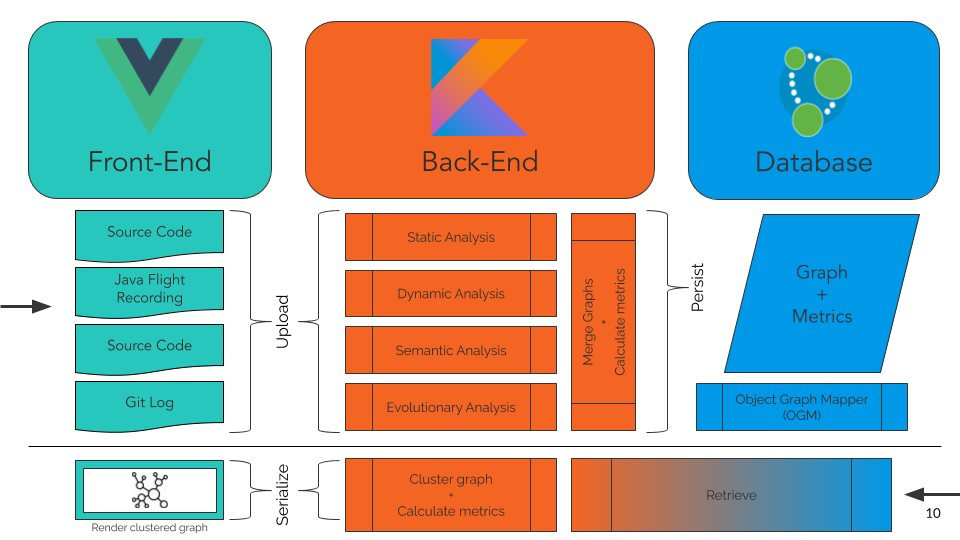
\includegraphics[width=.96\textwidth]{architecture-overview}
\caption{Overview of the architecture of our implementation}
\caption*{\centering
    The implementation is built as a three-tier web-based architecture consisting of
    front-end, back-end, and database. In the diagram, the two main functionalities of
    persisting and clustering input monolithic applications are depicted and
    divided by the horizontal black line.
}
\label{fig:architecture-overview}
\end{figure}



\section{Database} \label{sect:implementation-database}

As pointed out in the beginning of this chapter, a three-tier, web-based
application architecture was chosen which incorporates a database
for persistent data.
Instead of utilizing a traditional, relational database model,
for our implementation, the graph-based database model was chosen
due to the fact that the persisted data is entirely graph-based.
Thus, a graph-based database storage lends itself perfectly to the
type of data that we need to persist.

Graph databases are a subset of \textit{NoSQL} databases as they are
neither relational nor work with the \textit{Structured Query Language} (SQL)
\cite{vicknair2010graphdatabase}.
As Vicknair et al. show in their work \textit{A Comparison of a
Graph Database and a Relational Database}, when querying graph-based
data via a graph database compared to a relational, SQL-based
database management system (DBMS), the duration per query is oftentimes
drastically lower \cite{vicknair2010graphdatabase}.
Additionally, data modeling in the traditional sense is not even
necessary as the generated data can be persisted into the database as-is.
Due to these two reasons, especially the latter one, a graph-based DBMS
was chosen for our implementation.

Similarly to other database models, a multitude of DBMS exist following a
graph-based approach.
We chose the graph database \textit{Neo4j} for the following two reasons.
Firstly, it is by far the most popular and most well-maintained graph DBMS
\cite{graph-dbms-ranking}.
Secondly, it is implemented in Java and provides an API library for Java
and additionally an \textit{Object Graph Mapper} (OGM) which is a library
that can map the graph model into native Java objects with built-in
serialization and deserialization just as an \textit{Object Relational Mapper} (ORM)
would \cite{neo4j-ogm}.


\subsection{Object graph mapper}

To utilize the \textit{Neo4j} OGM, written and maintained by the \textit{Neo4j}
creators \cite{neo4j-ogm}, one composes classes for each node and edge type
that is used. Within \textit{Neo4j}, these are called \textit{Nodes} and
\textit{Relationships} \cite{neo4j-ogm}.
In the following subsections, the process of building OGM models and utilizing
them is exhibited.


\subsubsection{Relationships}
One has to create a class annotated with \code{@RelationshipEntity("")},
the annotation itself is part of the OGM library and has to be imported.
A class annotated like this can then be used to serialize and deserialize edges
of the respective graph. The annotation needs to know what the type of the
\textit{Relationship} is, this is a string that is necessary since \textit{Neo4j}
persists the edges of the input graph as the mentioned \textit{Relationships}.
Precisely, the \textit{Neo4j} creators recommend to use single uppercase third-person
singular present tense verbs to describe the type of relation \cite{neo4j-ogm}.
Thus, \code{"CALLS"}, \code{"OWNS"}, \code{"KNOWS"} would
be good examples. Due to this implementation detail of \textit{Neo4j},
this information has to be provided when annotating \textit{Relationship} classes.
The rest of the created class are just properties, some of which are mandatory,
while as many additional ones containing data can be added arbitrarily.

\begin{lstlisting}[caption=Relationship OGM class, label=ogm-relationship, breaklines=true]
@RelationshipEntity(type = CALLS)
class CallsRelationship() {
    @Id
    @GeneratedValue
    var id: Long? = null

    @StartNode
    var caller: Unit

    @EndNode
    var callee: Unit

    @Property
    var dynamiCouplingScore: Int = 0

    @Property
    var semanticCouplingScore: Int = 0

    @Property
    var logicalCouplingScore: Int = 0
}
\end{lstlisting}

The above code example \ref{ogm-relationship}, is implemented in Kotlin,
as this programming language was used to implement the entire back-end,
as discussed earlier in this chapter.
The class identifier can be chosen arbitrarily while the class needs to
encompass three properties.
Namely, these are \code{@StartNode}, \code{@EndNode}, and \code{@Id}.
The annotations \code{@StartNode} and \code{@EndNode} need to point
to a non-nullable instance of a \textit{Node} class as exhibited in the
following subsection. As the naming implies, this information is used
to link the resulting edge of this \textit{Relationship} class to the
two vertices that it connects.
Moreover, the \code{@Id} annotation is used to have a unique identifier
once an object of the class gets instantiated so that the OGM can map
the object back to the object in the persistent graph data storage.
Either the developer supplies these identifiers from the outside although
it is advised to just leverage the \code{@GeneratedValue} annotation that
will handle all this mapping automatically \cite{neo4j-ogm}.
When utilizing the OGM library within Kotlin, this property has to be
declared to be nullable owing to the fact that the identifier might not
be known when creating and subsequently inserting a completely new entity.
Finally, one can add an arbitrary amount of additional data properties
to the class via the \code{@Property} annotation since \textit{Neo4j} can persist
any data together with any \textit{Relationship}. In our use case,
these are the coupling scores discussed in section \ref{sect:software-quality-metrics}.
The entirety of the modeled data is covered at the end of this section in
\ref{subsect:data-models}.


\subsubsection{Nodes}
Similarly to the \textit{Relationships}, the \textit{Nodes} are also
created by annotating a class, this time with the \code{@NodeEntity}
annotation. Again, certain properties on the defined class are mandatory
while others can be added optionally as seen in code example \ref{ogm-node}.
\begin{lstlisting}[caption=Node OGM class, label=ogm-node, breaklines=true]
class Unit(
    var identifier: String,
    var packageIdentifier: String,
    var projectName: String,
    var size: Long
) {
    @Id
    @GeneratedValue
    override var id: Long? = null

    @Relationship(type = CALLS, direction = INCOMING)
    var callees: MutableSet<CallsRelationship> = mutableSetOf()

    @Relationship(type = CALLS, direction = OUTGOING)
    var callers: MutableSet<CallsRelationship> = mutableSetOf()
}
\end{lstlisting}
The \code{@Id} is required once again while the \code{@Relationship}
annotations are not mandatory, nevertheless a node in a given graph usually
has outgoing or incoming edges (or unidirectional or undirected ones).
Since all relationships in \textit{Neo4j} have to be directional but
the graph that is constructed as part of our methodology is undirected,
the directions out of the merged, final graph are used.
Importantly, during further steps or after retrieval out of \textit{Neo4j},
these directions are ignored via the \code{.equals()} and \code{.hashCode()}
methods of the custom data class representing an edge of a graph.
Moreover, similarly to \textit{Relationships} in \textit{Neo4j}, every \textit{Node}
can optionally carry an arbitrary number of additional data fields which are set
via regular class properties in the constructor in example \ref{ogm-node}.
Finally, the \textit{Nodes} as well as the \textit{Relationships} can have additional
methods, these are ignored by the OGM as it just looks for properties.


\subsubsection{Persisting and retrieving graph data}
A \code{SessionFactory} that is shipped with the OGM library returns
\code{Session} objects that among others offer the methods:
\begin{itemize}[noitemsep]
    \item \code{save()}
    \item \code{loadAll()}
\end{itemize}
The first one accepts any class instance annotated with the \code{@NodeEntity}
or \code{@RelationshipEntity} annotation and persists it into the \textit{Neo4j}
database. Additionally, serialization and subsequent mapping of native JVM
data types into data types supported by \textit{Neo4j} is completely automatic
and handled by the OGM \cite{neo4j-ogm} although both can be configured manually
if wished. Furthermore, the OGM will recursively persist the data attached to the
object passed into the \code{save()} method (e.g. a \textit{Node} connected to
another one via a \textit{Relationship}, all three will be persisted).
The second method can in return retrieve already persisted data.
Its API allows for ordering, pagination, filtering, and other features \cite{neo4j-ogm},
although our implementation only makes use of the filtering features, such as
\code{session.loadAll(Unit.class, Filter("projectName", ComparisonOperator.EQUALS, "test"))}.
Once again, the deserialization and mapping of the data types is handled by
the OGM by passing it a static reference to an annotated OGM entity class.


\subsection{Data models} \label{subsect:data-models}

Finally, the devised data models for our implementation are covered in this subsection.
Overall, only one \textit{Relationship} and only two \textit{Nodes} are necessary
to model our data as depicted in figures \ref{fig:data-models-nodes} and
\ref{fig:data-models-relationships}.

\begin{figure}[htbp]
\centering
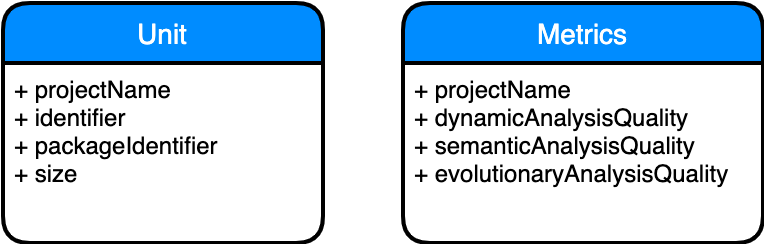
\includegraphics[width=.90\textwidth]{data-models-nodes}
\caption{Node data models}
\caption*{\centering
  Two \textit{Node} models are necessary. The first one carries the extracted
  data while the second one is used to persist the calculated metrics on a
  per\hyp project basis.
}
\label{fig:data-models-nodes}
\end{figure}

\begin{figure}[htbp]
\centering
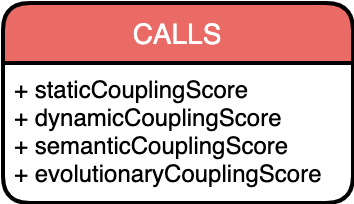
\includegraphics[width=.50\textwidth]{data-models-relationships}
\caption{Relationships data models}
\caption*{\centering
  One \textit{Relationship} model is necessary. Its sole usage is to link
  two \code{Unit} \textit{Nodes} together as seen in figure \ref{fig:data-models-nodes}.
}
\label{fig:data-models-relationships}
\end{figure}

\begin{figure}[htbp]
\centering
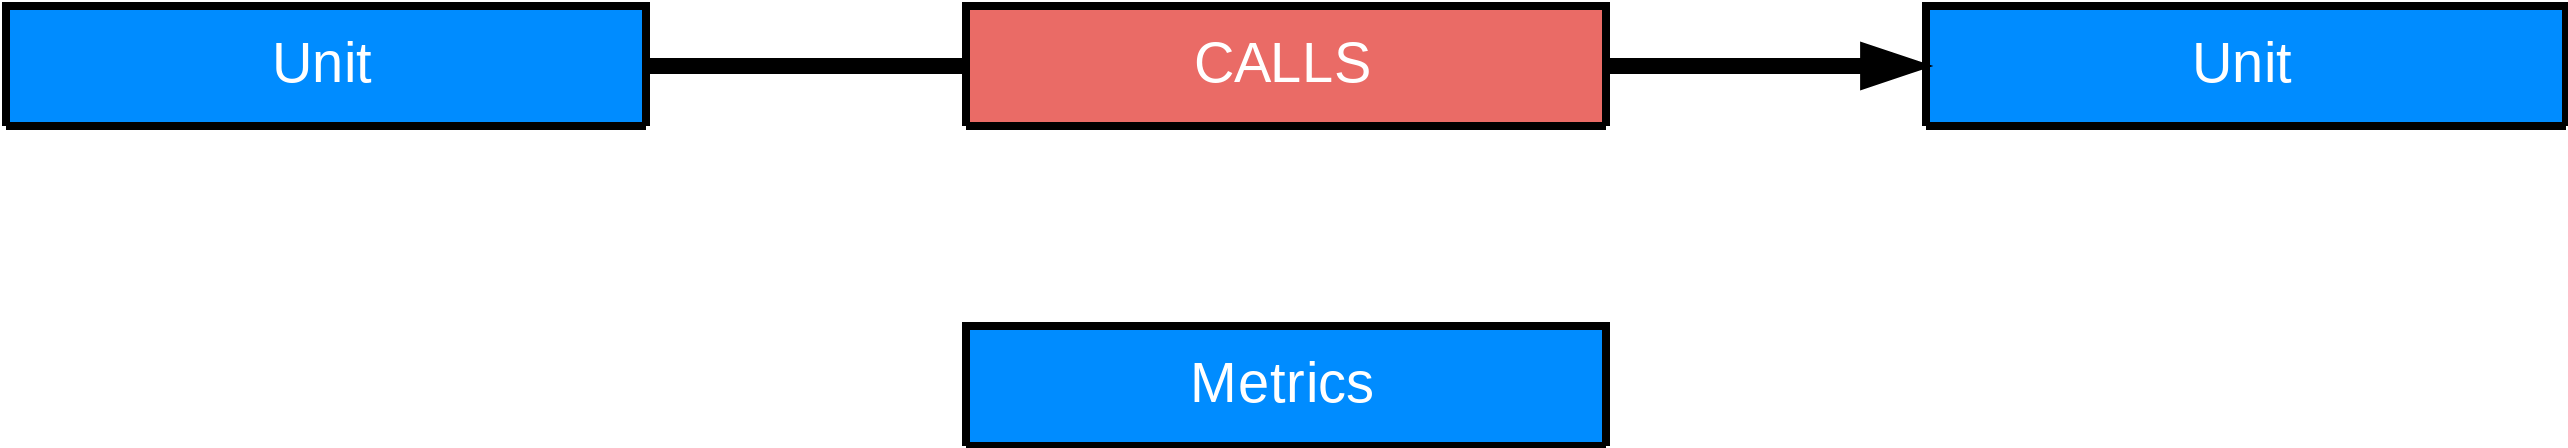
\includegraphics[width=.90\textwidth]{data-models-example}
\caption{Data models example}
\caption*{\centering
  This is an example how the \textit{Nodes} and \textit{Relationships} work together.
}
\label{fig:data-models-example}
\end{figure}

Precisely, the \code{Metrics} \textit{Node} persists metrics on a per\hyp project basis
as described in section \ref{sect:input-fidelity-metrics} --- only the fidelity
metrics are persisted in the database owing to the fact that their calculation is
resource\hyp intensive thus the result is persisted as it will not change in any case.
The \code{Unit} \textit{Node} is the main \textit{Node} type of the data model as it
encompasses the graph that was constructed out of the input
monolithic application as exhibited in chapter \ref{chap:extracting-coupling}.
The \code{CALLS} \textit{Relationship} is used to persist which
\code{Unit} \textit{Nodes} are linked to each other.
Finally, figure \ref{fig:data-models-example} depicts how the modeled
\textit{Nodes} and \textit{Relationships} behave while figure \ref{fig:class-diagram-graph-entity}
depicts a class diagram of the involved classes within the back-end.

\begin{figure}[htbp]
\centering
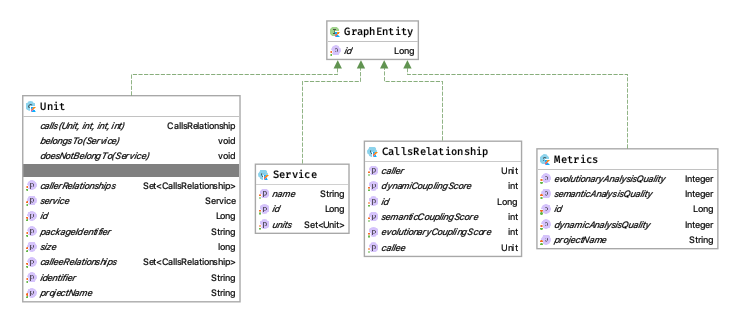
\includegraphics[width=\textwidth]{class-diagram-graph-entity}
\caption{Class diagram of the classes involved in the data model}
\caption*{\centering
  Each node and relationship type in \textit{Neo4j} is modeled as a class
  in the back-end.
}
\label{fig:class-diagram-graph-entity}
\end{figure}



\section{Back-end} \label{sect:implementation-back-end}

As already shown, the entire back-end is implemented in the programming language
\textit{Kotlin} which is a language heavily based on Java, that compiles to JVM
bytecode while also being completely inter-operable with Java code meaning that
any existing Java libraries can seamlessly be used within Kotlin source code.

The back-end is built as a web-based application with a RESTful API that offers
a couple of endpoints for the front-end to use and consume.
The server process is utilizing \textit{Netty} \cite{ktor-netty} as an embedded
server although the native coroutines of Kotlin are used to spawn a new one for
every incoming HTTP request.
Furthermore, coroutines are used within the business logic as well.
\textit{Coroutines} are a feature of the Kotlin language which are a lightweight
abstraction on top of threads that enable asynchronous programming \cite{kotlin-coroutines}.
The starting point of said server process is the file \textit{Main.kt} that
performs all of the scaffolding and starts up the server back-end.

For the API endpoints, the so-called \textit{resources}, a library called
\textit{Ktor} was utilized which enables easy declaration and configuration
of them. The library is built and maintained by the Kotlin creator
\textit{JetBrains} \cite{ktor}.
All endpoints accept and respond via \textit{JSON} as the data exchange format
while the library \textit{Jackson} is used to automatically serialize and
deserialize JSON data \cite{ktor-jackson}.

Going deeper into the back-end from the endpoints, \textit{controllers} are handling
the request and instantiate and call the respective parts of the business logic.

Moreover, a \textit{models} directory holds all the classes that are used
as \textit{data classes} as they are called in Kotlin --- classes that are not
encapsulating any advanced business logic and are instead used to pass data around
the application in a structured way. Additionally, some may offer static utility
methods specific to their usage or when leveraging a special data format that
needs to be converted from other formats.

Finally, some functionalities are small in size and are used by multiple parts
of the business logic hence have no natural location in the application structure.
These \textit{utility} classes are therefore residing in a directory called
\textit{utility} in the top-level of the application structure.
The top-level structure of the application is depicted in figure
\ref{fig:back-end-structure} while a detailed explanation of every implemented
class can be found in the wiki of \textit{Steinmetz}
\footnote{\url{https://github.com/loehnertz/Steinmetz/wiki}}.

\begin{figure}[htbp]
\centering
\begin{forest}
  for tree={
    font=\ttfamily,
    grow'=0,
    child anchor=west,
    parent anchor=south,
    anchor=west,
    calign=first,
    edge path={
      \noexpand\path [draw, \forestoption{edge}]
      (!u.south west) +(7.5pt,0) |- node[fill,inner sep=1.25pt] {} (.child anchor)\forestoption{edge label};
    },
    before typesetting nodes={
      if n=1
        {insert before={[,phantom]}}
        {}
    },
    fit=band,
    before computing xy={l=15pt},
    inner sep=0.75pt,
  }
[kotlin
  [controller
    [analysis]
  ]
  [model
    [graph]
    [metrics]
    [neo4j]
    [resource]
  ]
  [resource
    [AnalysisResource.kt]
  ]
  [utility
    [ArchiveExtractor.kt]
    [Neo4jConnector.kt]
    [Utilities.kt]
  ]
  [Main.kt]
]
\end{forest}
\caption{Top-level back-end structure}
\caption*{\centering
  The top-level file structure of the back-end with a maximum depth of 3.
}
\label{fig:back-end-structure}
\end{figure}


\subsection{API resources} \label{subsect:api-resources}

Namely, there are three resource endpoints for adding new projects, retrieving them,
and to eventually cluster them:
\begin{enumerate}[noitemsep]
    \item \code{GET \quad  "/analysis/"}
    \item \code{POST\quad  "/analysis/"}
    \item \code{GET \quad  "/analysis/\{projectName\}"}
    \item \code{GET \quad  "/analysis/\{projectName\}/cluster"}
    \item \code{GET \quad  "/analysis/\{projectName\}/optimize"}
\end{enumerate}


\subsubsection{Resource 1}
The first resource just responds with a list of names of all the projects that
have been analyzed in the past using resource 2.

This feature is used in the front\hyp end as well to provide an auto\hyp completing
search bar when entering a project name.


\subsubsection{Resource 2}
The second resource only accepts \code{POST} requests and is solely used to
create new projects by uploading the necessary data and extracting the
coupling information out of it as discussed in chapter \ref{chap:extracting-coupling}.
An overview of the data that resource 2 mandates is depicted in table
\ref{table:data-resource-1}.
Additionally, table \ref{table:binary-data-resource-1} exhibits what the
binary data fields of table \ref{table:data-resource-1} have to be in
the example case that \code{"JAVA"} was chosen as the \code{projectPlatform}.
Finally, we added a feature that allows for one of the three following
data fields to be missing during the upload owing to the fact that sometimes
it is difficult to supply all three (specifically the \code{dynamicAnalysisFile})
while the analysis can still be performed albeit with lower quality:
\begin{itemize}[noitemsep]
    \item \code{dynamicAnalysisFile}
    \item \code{semanticAnalysisFile}
    \item \code{evolutionaryAnalysisFile}
\end{itemize}

\begin{table}[ht!]
\smaller
\def\arraystretch{1.55}
\begin{tabularx}{\textwidth}{|Y|Y|Y|}
 \hline
 Name~ & Data type~ & Description~ \\
 \hline\hline
 \code{projectName}                & String &
 A freely chosable identifier for the uploaded data \\\hline
 \code{projectPlatform}            & Enum \{"JAVA"\} &
 The platform of the input monolithic application \\\hline
 \code{vcsSystem}                  & Enum \{"GIT", "HG", "SVN", "P4", "TFS"\} &
 The VCS system used during the development of the input monolithic application \\\hline
 \code{basePackageIdentifier}      & String &
 The root package identifier that all other packages in the project share; is used to filter out dependencies bundled with the application \\\hline
 \code{staticAnalysisFile}         & Binary &
 A binary file containing the data for performing the static analysis \\\hline
 \code{dynamicAnalysisFile}        & Binary &
 A binary file containing the data for performing the dynamic analysis \\\hline
 \code{semanticAnalysisFile}       & Binary &
 A binary file containing the data for performing the semantic analysis \\\hline
 \code{evolutionaryAnalysisFile}   & Binary &
 A binary file containing the data for performing the evolutionary analysis \\\hline
\end{tabularx}
\caption{Data required by resource 1}
\caption*{\centering
  The data that resource 1 (\code{POST "/analysis/"}) mandates to function.
}
\label{table:data-resource-1}
\end{table}

\begin{table}[ht!]
\smaller
\def\arraystretch{1.55}
\begin{tabularx}{\textwidth}{|Y|Y|Y|}
 \hline
 Name~ & File extension~ & Description~ \\
 \hline\hline
 \code{staticAnalysisFile}         & \code{.zip} &
 A \code{.zip} file with uncompiled source code\\\hline
 \code{dynamicAnalysisFile}        & \code{.jfr} / \code{.txt} &
 The \code{.jfr} extension stems from the \textit{Java Flight Recorder} which is a profiler shipped with newer
 JRE versions that can be enabled to conduct dynamic program analysis; the JRE also offers an API to process
 recorded \code{.jfr} files from within another Java application.
 Alternatively, a plain text file can be provided with each line resembling one method
 invocation. \\\hline
 \code{semanticAnalysisFile}       & \code{.zip} &
 Strictly needs the source code archived as a \code{.zip} file as the code written by the programmers
 is necessary to perform natural language processing. \\\hline
 \code{evolutionaryAnalysisFile}   & \code{.txt} &
 The format is depending on which \code{vcsPlatform} was chosen; a log file of the repository of that platform of the application as a plain text file. \\\hline
\end{tabularx}
\caption{Description of the binary data required by resource 1}
\caption*{\centering
  The binary data that resource 1 (\code{POST "/analysis/"}) mandates to function
  in the case of the Java platform chosen as the \code{projectPlatform}.
}
\label{table:binary-data-resource-1}
\end{table}


\subsubsection{Resource 3}
The third resource, \code{GET "/analysis/\{projectName\}"}, is solely used to
retrieve a project that was persisted earlier via resource 2. Hence, it only
mandates the \code{projectName} as a string to query \textit{Neo4j} for the
respective un\hyp clustered graph.


\subsubsection{Resource 4}
The fourth resource is used to cluster a graph that was persisted earlier using
resource 2. This is done in two steps as the computational time of the logic
behind resource 2 is a lot higher compared to the duration of the clustering
of resource 4. Furthermore, the clustering is usually performed multiple times
leveraging different graph clustering algorithms. Thus, it conserves resources
to construct the graph-theoretic representation of the input monolithic application
only once and to retrieve it multiple times for every request to resource 4.


\subsubsection{Resource 5}
The last resource is used to optionally optimize the hyper\hyp parameters of our methodology.
This is explained in more detail in subsection \ref{subsubsect:hyper-parameter-optimization}.


\subsection{Logic controllers}

Technically, only one logic controller exists, the \code{AnalysisController}, that
branches out into separate classes that implement the actual logic.
Figure \ref{fig:top-level-logic-structure} depicts the structure of the directories
containing the logic.
The \code{AnalysisController} class implements the actual controller for all of the
\code{"/analysis"} resources covered in subsection \ref{subsect:api-resources}.
From there, the \code{analysis} controller package branches out into three sub-packages
which are detailed in the following subsections.

\begin{figure}[htbp]
\scriptsize
\centering
\begin{minipage}{0.5\linewidth}
\begin{forest}
  for tree={
    font=\ttfamily,
    grow'=0,
    child anchor=west,
    parent anchor=south,
    anchor=west,
    calign=first,
    edge path={
      \noexpand\path [draw, \forestoption{edge}]
      (!u.south west) +(7.5pt,0) |- node[fill,inner sep=1.25pt] {} (.child anchor)\forestoption{edge label};
    },
    before typesetting nodes={
      if n=1
        {insert before={[,phantom]}}
        {}
    },
    fit=band,
    before computing xy={l=15pt},
    inner sep=0.75pt,
  }
[analysis
  [clustering
    [chinesewhispers
        [ChineseWhispersManager.kt]
    ]
    [clausetnewmanmoore
        [ClausetNewmanMooreManager.kt]
    ]
    [infomap
        [InfomapManager.kt]
    ]
    [labelpropagation
        [LabelPropagationManager.kt]
    ]
    [louvain
        [LouvainManager.kt]
    ]
    [mcl
        [MclExecutor.kt]
        [MclManager.kt]
    ]
    [walktrap
        [WalktrapExecutor.kt]
        [WalktrapManager.kt]
    ]
    [AbstractNeo4jAlgorithmManager.kt]
    [Clusterer.kt]
    [ClusteringAlgorithm.kt]
    [ClusteringAlgorithmManager.kt]
    [EdgeWeightingFormulaCalculator.kt]
  ]
  [extraction
    [coupling
        [dynamically]
        [evolutionary]
        [semantically]
        [statically]
    ]
    [graph
        [GraphConverter.kt]
        [GraphInserter.kt]
    ]
    [AbstractExtractor.kt]
    [ExtractorCompanion.kt]
    [Platform.kt]
  ]
  [metrics
    [clustering
        [ClusteringQualityAnalyzer.kt]
    ]
    [input
        [InputQualityAnalyzer.kt]
    ]
  ]
  [optimization
    [genetic
        [EvolutionManager.kt]
        [Specimen.kt]
    ]
  ]
  [AnalysisController.kt]
]
\end{forest}
\end{minipage}
\caption{Structure of the packages containing the logic}
\caption*{\centering
  The top-level file structure of the packages that contain the implemented
  business logic with a maximum depth of 4.
}
\label{fig:top-level-logic-structure}
\end{figure}


\subsubsection{Clustering}
This package contains everything necessary to perform the clustering of
earlier uploaded projects. As exhibited in section \ref{sect:graph-clustering-algorithm-survey},
seven graph clustering algorithms were implemented by wrapping the
reference implementations of their authors in a generic API that is consistent
within our implementation for all of the utilized graph clustering algorithms.

\paragraph{Clusterer.kt}
The \code{Clusterer} class is the entry point for clustering an input graph
using any of the available algorithms. The graph that was retrieved out of
\textit{Neo4j} is passed into the \code{Clusterer} after being cloned owing
to the fact that by default, all of the available algorithms will concurrently
cluster the selected graph such that all of them would work on the same
reference in memory which would cause corruption.

\paragraph{ClusteringAlgorithm.kt}
This file contains an enum which is used to identify which graph clustering
algorithm the \code{Clusterer} should apply to the input graph.

\paragraph{ClusteringAlgorithmManager.kt}
This file contains an interface which defines a contract that all of the
distinct manager classes for each available graph clustering algorithm
should implement --- it ensures that the APIs for all of the algorithms stay consistent.

\paragraph{EdgeWeightingFormulaCalculator.kt}
This file contains a class with static methods that implement the edge weighting
which was detailed in section \ref{sect:merging-graphs}.

\paragraph{Graph clustering managers and executors}
Every sub-package for each of the available graph clustering algorithms contains
a manager class which implements the \code{ClusteringAlgorithmManager} interface.
In these classes, the actual reference implementation of each algorithm is wrapped.
Consequently, the implementations in those classes differ vastly from one to the other.
A class diagram has been created to depict the classes involved in this step
(see figure \ref{fig:class-diagram-clustering-algorithm-manager}).

\begin{figure}[htbp]
\centering
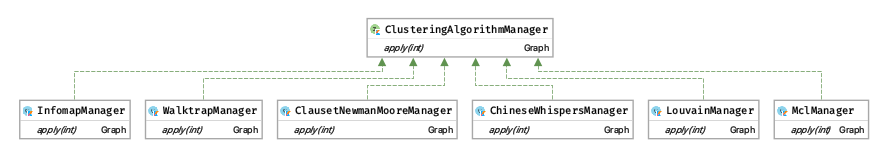
\includegraphics[width=\textwidth]{class-diagram-clustering-algorithm-manager}
\caption{Class diagram of the major classes involved in the clustering step}
\caption*{\centering
  All of the supported graph clustering algorithms have a class that implements
  their usage.
}
\label{fig:class-diagram-clustering-algorithm-manager}
\end{figure}

Some of the reference implementations are written in Java which allows us to directly
integrate them into our implmentation. However, the majority of them are compiled C or
C++ programs that are more difficult to integrate.
Initially, we leveraged the \textit{Java Native Interface} (JNI), a foreign function
invocation interface bundled with the Java platform, that can be used to integrate
C, C++, and assembly programs into a Java application \cite{jni}.
On the downside, the source code of the C and C++ programs has to be modified to utilize
the JNI. However, we did not have access to all of the reference implementations as source
code, some were only shipped pre-compiled.
Moreover, all of the reference implementations in C or C++ are designed as
\textit{Command Line Interfaces} (CLI) instead of libraries.
As a consequence, in the latest version of \textit{Steinmetz}, we opted to wrap the
CLI with the \code{ProcessBuilder} class of the Java platform \cite{process-builder}.
This enables to call any CLI from within a Java application by invoking a process,
piping input into \code{STDIN} and parsing the output of the invoked program from
the processes \code{STDOUT}. This might seem error-prone on first sight, however,
the CLIs are all well-defined which makes input and output of them easy to
encode and decode.
Additionally, we added a lot of validation for the input such that we have not seen
an error or malfunction when testing and evaluating our implementation so far.
The only downside is that the portability of the Java platform is lowered a bit,
as the compiled native programs are platform-specific. Nevertheless, the same problem
is present when using the JNI.

Furthermore, some graph clustering algorithms mandate multiple runs to yield good results.
Thus, an additional executor class is utilized there which contains the actual logic while
the manager class wraps the executor class and executes multiple instances of it concurrently,
leveraging the \textit{coroutine} feature of the Kotlin programming language.


\subsubsection{Extraction}
The sub-packages within the package \code{extraction.coupling} in figure
\ref{fig:top-level-logic-structure} are each implementing one input dimension of the
ones highlighted in chapter \ref{chap:extracting-coupling}.
A class diagram of the involved classes can be seen in figure
\ref{fig:class-diagram-abstract-extractor}.

\begin{figure}[htbp]
\centering
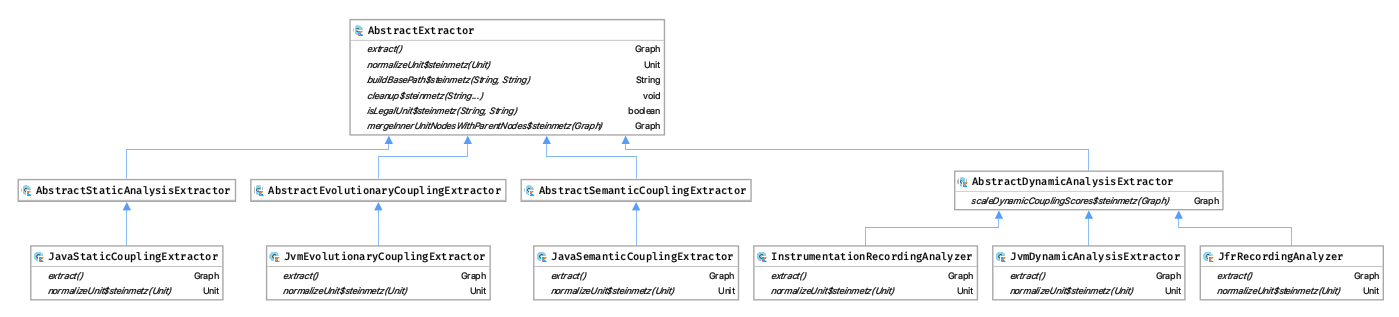
\includegraphics[width=\textwidth]{class-diagram-abstract-extractor}
\caption{Class diagram of the classes involved in the extraction step}
\caption*{\centering
  Every of the four coupling dimensions gets a class that implements it
  for a supported platform.
}
\label{fig:class-diagram-abstract-extractor}
\end{figure}

Firstly, the sub-package \code{extraction.graph} contains two classes,
\code{GraphConverter} and \code{GraphInserter}, which are handling the deserialization
of a graph retrieved out of \textit{Neo4j} utilizing the OGM and the insertion of
a newly constructed graph into \textit{Neo4j} respectively.

As pointed out earlier, the extraction strategies differ from platform to platform.
Thus, for illustrative purposes, we implemented the entire flow for the \textit{Java}
platform. The \code{Platform.kt} file contains an enum with all of the available
platforms --- currently only \code{JAVA}. However, later in this section we show
how our implementation can be easily extended for other platforms as this was a
conscious design decisions to model the architecture in an extendable manner.
This enum is used by the controller to know which classes to instantiate and invoke
that then conduct the coupling extraction.

Moreover, the \code{AbstractExtractor} and \code{ExtractorCompanion} are an abstract
class and an interface that all of the extraction classes respectively their
static companions implement. \textit{Companions} are a feature of the Kotlin language
that allow to create static methods by embedding a singleton object within a class
that can therefore stay stateless and static \cite{kotlin-companions}.

Within each of the mentioned sub-packages, there is an abstract class that implements
some general behavior necessary for the respective input dimension
(e.g. \code{AbstractDynamicAnalysisExtractor}). The abstract class itself however
implements the \code{AbstractExtractor}.
Within each of the sub-packages, there are sub-packages for each platform available
in the \code{Platform} enum.
In this chapter, the exact implementation of all of these is not covered as the
explanation would be very detailed. Instead, only one type of coupling extraction
will be covered for the sake of example. All of the others can be studied via the
source code itself or via the documentation.
Furthermore, the entire structure of the coupling extraction is depicted in figure
\ref{fig:coupling-extraction-structure}.

\paragraph{JavaSemanticCouplingExtractor.kt}
For the semantic coupling extraction, we opted to build our own implementation
from scratch. As according to the process exhibited in \ref{subsect:semantic-similarity},
we implemented a completely decoupled library that calculates \textit{semantic similarity}
of input code bases. Similarly to the main implementation of our methodology,
the Java platform was implemented for now again, the extendability regarding other
platforms however is easily possible and encouraged.

The library has the simple name \textit{semantic-coupling} and is available as
open source code on GitHub, licensed under the \textit{MIT license}
\footnote{\url{https://github.com/loehnertz/semantic-coupling/}}.
Additionally, we plan on releasing it on \textit{Maven Central} after the release
of this thesis. The library is completely separate from our methodology and
also generic in its implementation.

The \code{main} method accepts a list of documents as plain-text strings,
the source code files, as well as the programming language that they are written in
out of an included public enum.
The returned result is a list of tuples with the two source code files that were compared
as well as their percentage-based similarity as a floating point number.

Additionally, many options can be set when constructing the public entry class
of the library. These include if \textit{stemming} or \textit{lemmatization} should be used,
if \textit{LSI} should be used, if so, how many \textit{LSI} dimensions should be calculated,
and if certain source code files should be excluded to gain some execution speed if the user
is not interested in their similarity anyways.

Furthermore, the aforementioned Kotlin \textit{coroutines} are heavily leveraged in
the library as many steps of the \textit{semantic similarity} calculation can be
run concurrently.

\begin{figure}[htbp]
\small
\centering
\begin{forest}
  for tree={
    font=\ttfamily,
    grow'=0,
    child anchor=west,
    parent anchor=south,
    anchor=west,
    calign=first,
    edge path={
      \noexpand\path [draw, \forestoption{edge}]
      (!u.south west) +(7.5pt,0) |- node[fill,inner sep=1.25pt] {} (.child anchor)\forestoption{edge label};
    },
    before typesetting nodes={
      if n=1
        {insert before={[,phantom]}}
        {}
    },
    fit=band,
    before computing xy={l=15pt},
    inner sep=0.75pt,
  }
[extraction.coupling
  [dynamically
    [platforms
        [java
            [InstrumentationRecordingAnalyzer.kt]
            [JfrRecordingAnalyzer.kt]
            [JvmDynamicAnalysisExtractor.kt]
        ]
    ]
    [AbstractDynamicAnalysisExtractor.kt]
  ]
  [evolutionary
    [platforms
        [java
            [JvmLogicalCouplingExtractor.kt]
        ]
    ]
    [AbstractLogicalCouplingExtractor.kt]
    [VcsPlatform.kt]
  ]
  [semantically
    [platforms
        [java
            [JavaSemanticCouplingExtractor.kt]
        ]
    ]
    [AbstractSemanticCouplingExtractor.kt]
  ]
  [statically
    [platforms
        [java
            [JvmBytecodeExtractor.kt]
        ]
    ]
    [AbstractStaticAnalysisExtractor.kt]
    [StaticAnalysisExtractorCompanion.kt]
  ]
]
\end{forest}
\caption{Structure of the packages containing the coupling extraction logic}
\caption*{\centering
  The file structure of the packages that contain the implemented coupling extraction logic.
}
\label{fig:coupling-extraction-structure}
\end{figure}


\subsubsection{Metrics}
This package contains two sub-packages which each contain classes that implement
the calculation of the metrics for the input and the clustering respectively,
as detailed in chapter \ref{chap:metrics}.
The distinct implementations are not covered in more detail as they are very
close to the mathematical formulae in chapter \ref{chap:metrics}.


\subsubsection{Hyper-parameter optimization} \label{subsubsect:hyper-parameter-optimization}
Similarly to the fact that some graph clustering algorithms are run
multiple times concurrently to counteract the fact that they require the amount
of clusters a priori, we implemented a similar idea for the hyper\hyp parameters
of our methodology, namely the coupling type weights.

To keep the runtimes of the optimization acceptable, we opted to implement a
genetic algorithm that optimizes the hyper\hyp parameters \cite{eiben2003introduction}.
It serializes the three parameters (i.e. \textit{dynamic coupling weight},
\textit{semantic coupling weight}, \textit{evolutionary coupling weight}) into
a chromosome. By default, a population of size 100 is evolved over 100 generations.
To get out of local minima, the longer no better parameters were found, the higher
the mutation chance gets according to the following formula while the
$chanceToMutateInPercent$ is set to 1 by default and the $mutationChance$
is capped to 50\%:
\[
  \frac{(chanceToMutateInPercent \times generationsWithoutImprovement)}{2}
\]

In the front\hyp end, the user can select which graph clustering algorithm is
utilized for the fitness function of the genetic algorithm.
Additionally, the metric that is the output of the fitness function can be
selected from the available ones.


\subsection{Extending the analysis for a new language}

It was a conscious design decision in the engineering of the implementation that its core
is agnostic of any programming language or platform that it analyzes.
As seen in figure \ref{fig:coupling-extraction-structure}, the \code{extraction.coupling}
package contains sub\hyp packages for every coupling dimension and then another sub\hyp package
for the platforms that are supported. As described earlier, we exemplarily implemented every step
of the analysis of software written in Java, hence the \code{java} packages in each
\code{platforms} sub\hyp package.
To be able to analyze another language or platform, one has to conduct four steps:
\begin{enumerate}
    \item Implement each abstract extractor class for all of the four coupling dimensions
    \item Add the new language or platform to the \code{extraction.Platform} enum
    \item Add the new enum entry to the front-end so it becomes selectable
    \item Extend the clauses of the methods in \code{extraction.graph.GraphInserter}
\end{enumerate}



\section{Front-end} \label{sect:implementation-front-end}

The front-end is designed and built as a \textit{single page application} (SPA)
using \textit{Vue.js}, which is a framework to built reactive SPAs utilizing
HTML, CSS, and JS that run in a web browser \cite{vuejs}.

It supports and encourages to build the SPA as multiple, reusable components.
Thus, the engineer has to design up-front how the planned front-end could be
logically divided into components --- in this regard it takes ideas from
object orientation as one component can build upon other ones and inherit
and augment their functionality.

The framework contains control structures to render components conditionally
and to loop over an array data structure while rendering HTML and CSS for
every item in said array. Features like these are main arguments for utilizing
a SPA framework compared to building the front-end application from scratch
with plain HTML, CSS, and JS.
Yet, the most important feature is the built-in reactiveness which is not built
into web browsers. Precisely, it put watchers onto every usage of any state
in the SPA and automatically re-renders just the effected HTML node in the DOM
on-the-fly which allows the engineer to build applications that are reacting
to state changes on their own rather then via a manually implemented trigger
\cite{vuejs}.

Furthermore, every component has a transient state that vanishes upon a
page refresh or session reload by default. Each component can send messages,
mostly consisting of state updates, to child components that they embed as well
as to components higher up in the hierarchy.
As a consequence, one entry point component exists that the engineer fills
with other components to assemble the SPA.

The data to populate the components state and therefore the page is usually
fetched from an API endpoint of a back-end application, this is no different
in our case.


\subsection{User interface}

The user interface (UI) is arranged as a set of cards stacked on top of each
other. Either, they display control elements or rendered data.
Figure \ref{fig:front-end-ui} is a screenshot of the entire front-end with
example input and data. Every card has a clear and distinct border with
a shadow to visually separate them from each other.
In the following subsection, some of the most important cards are covered
in more detail. From top to bottom, the cards fulfill the following tasks:

\begin{enumerate}
  \item Adding a new project by uploading the analysis files. Additionally,
        the programming language as well the VCS platform of the input
        monolithic application have to be selected.
  \item Retrieving a project that was persisted earlier either as the plain
        graph or in its clustered form.
  \item Selecting a graph clustering algorithm for rendering the visualization
        below as well as selecting a metric that should be used for evaluating
        the results. Additionally, a slider sets how many runs graph clustering
        algorithms should get that are either non-deterministic or have an
        additional input parameter that determines the granularity of the
        resulting clustering. In that case, these algorithms are maximally run
        as often as the slider specifies in a concurrent manner.
  \item Changing the weighting for the three input dimensions. By default,
        every dimension is weighted the same, however, this can be changed by
        the user.
  \item The rendered graph either plain or clustered; every cluster then depicts
        one microservice. Furthermore, the connections between the units of the
        input monolithic application as part of the microservices can be
        examined. The view can zoomed seamlessly.
        Moreover, a completely textual view can alternatively be displayed.
  \item A brief overview of general metrics that are not specific to clustering.
  \item The metrics that are specific to the clustering and more specifically
        belonging to the graph clustering algorithm selected above.
  \item The same card as the one above for each of the available
        graph clustering algorithms apart from the selected one.
\end{enumerate}

\begin{figure}[htbp]
\centering
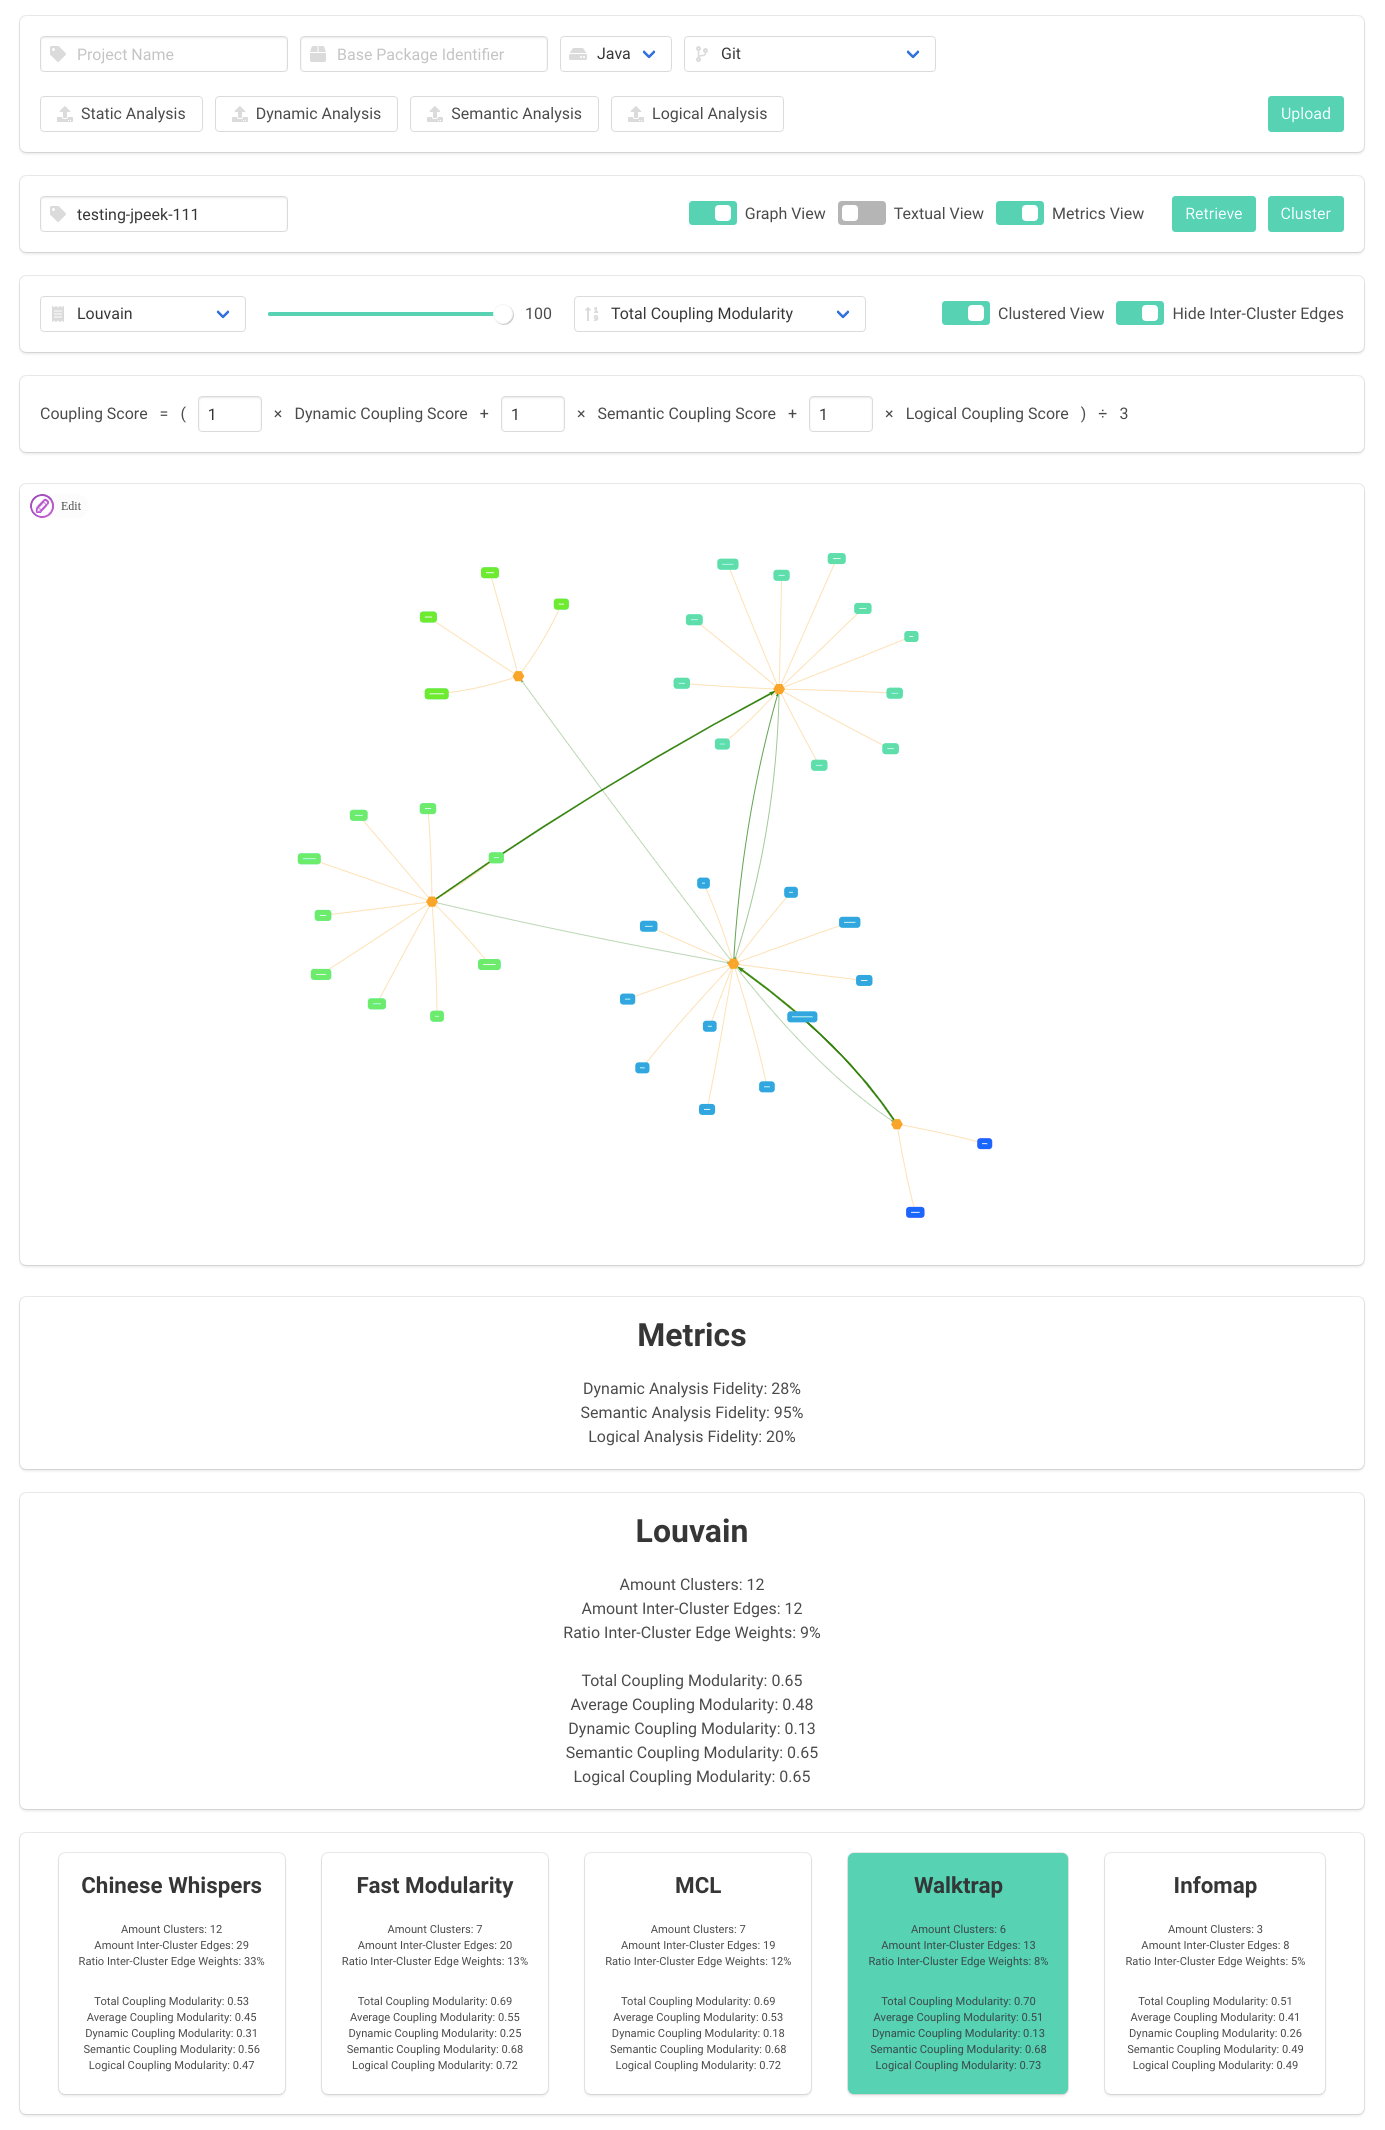
\includegraphics[width=\textwidth]{front-end-ui}
\caption{User interface of the front-end}
\caption*{\centering
  The front-end consists of multiple cards stacked on top of each other,
  each filled with either controls or displaying rendered data.
}
\label{fig:front-end-ui}
\end{figure}


\subsection{Visualizing microservice recommendations}

After uploading a new project or retrieving an existing one, three views exist
for visualizing features of the microservice recommendations for that project.
Selecting a graph clustering algorithm in the third tile of the UI
has the effect that the resulting clustering of the selected algorithm
will be used to render all of the views exhibited in this subsection.
Regardless of the selection, all of the available algorithms are executed
concurrently, but the selected one will provide the data for rendering the views.


\subsubsection{Graph view}
\begin{figure}[htbp]
\centering
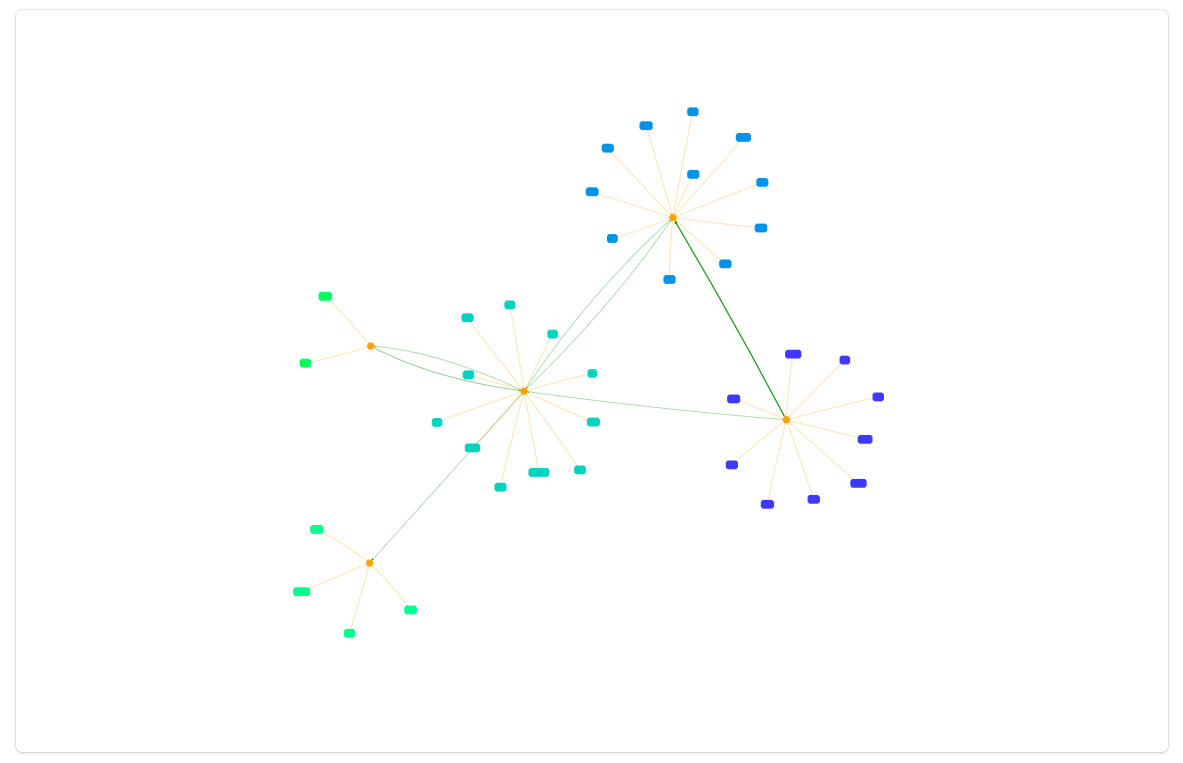
\includegraphics[width=.96\textwidth]{graph-view-ui}
\caption{The graph view in the UI of the front-end}
\caption*{\centering
  The front-end offers a \textit{graph view} of the clustered graph that depicts
  the computed microservice recommendations.
}
\label{fig:graph-view-ui}
\end{figure}

The first and most obvious view is the \textit{graph view}. It essentially
renders the graph that is already persisted in \textit{Neo4j} with the
computed clustering visualized as well. Figure \ref{fig:graph-view-ui} shows
the \textit{graph view} in detail. The whole view can be zoomed in and out
seamlessly by scrolling within the card. We tested the visualization with
a 10,000 node, fully-connected graph which was still functional although
rendered with a lower frame rate. The rendering is done via a HTML5 \code{<canvas>}.

\paragraph{Default mode}
Precisely, orange hexagons depict a microservice while the classes between
different microservices have different randomized colors to visually emphasize
them toward each other. The orange lines are intra-cluster connections,
while green lines are inter-cluster connections.
These have different thicknesses depending on their edge weight which can be
displayed by hovering over the edge. Moreover, the inter-cluster edges have
arrow heads depicting in which directions the microservices would invoke
each other which can be seen in detail in figure \ref{fig:node-graph-view}.
Finally, every unit of each service has its name printed inside of the node
as well as the fully qualified name and the byte size when hovering over it
as seen in figure \ref{fig:node-graph-view}.

\begin{figure}[htbp]
\centering
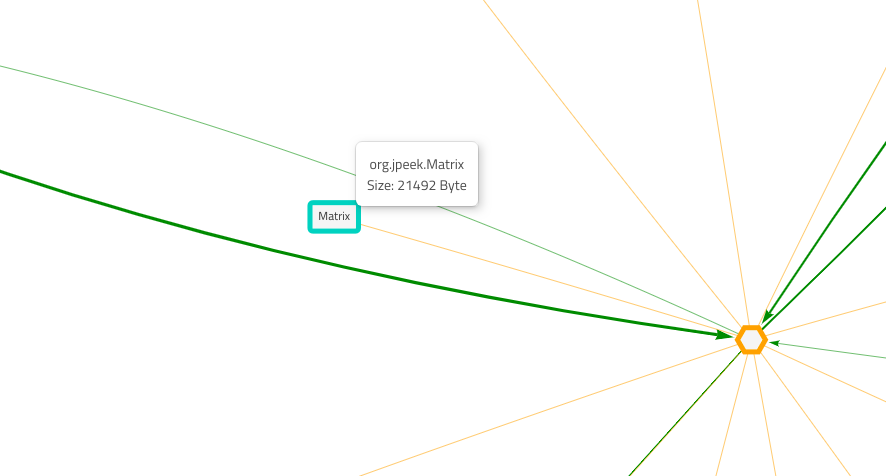
\includegraphics[width=.96\textwidth]{node-graph-view}
\caption{A closeup of a node in the graph view}
\caption*{\centering
  Every node's name is displayed once zoomed in far enough.
  Furthermore, when hovering over any node, additional information is displayed.
}
\label{fig:node-graph-view}
\end{figure}

\paragraph{Detailed mode}
Additionally, another mode of the view exists that will display intra-cluster
edges which allows the user to see how units within a service are connected
to each other as well as how they are connected to other services and their
units. Furthermore, units in a square shape are solely accessed within their
own service while units in a diamond shape are communicating with units from
other microservices.
This mode can be seen in figure \ref{fig:detailed-graph-view} and is
activated by toggling the \textit{Hide Inter-Cluster Edges} option.

\begin{figure}[htbp]
\centering
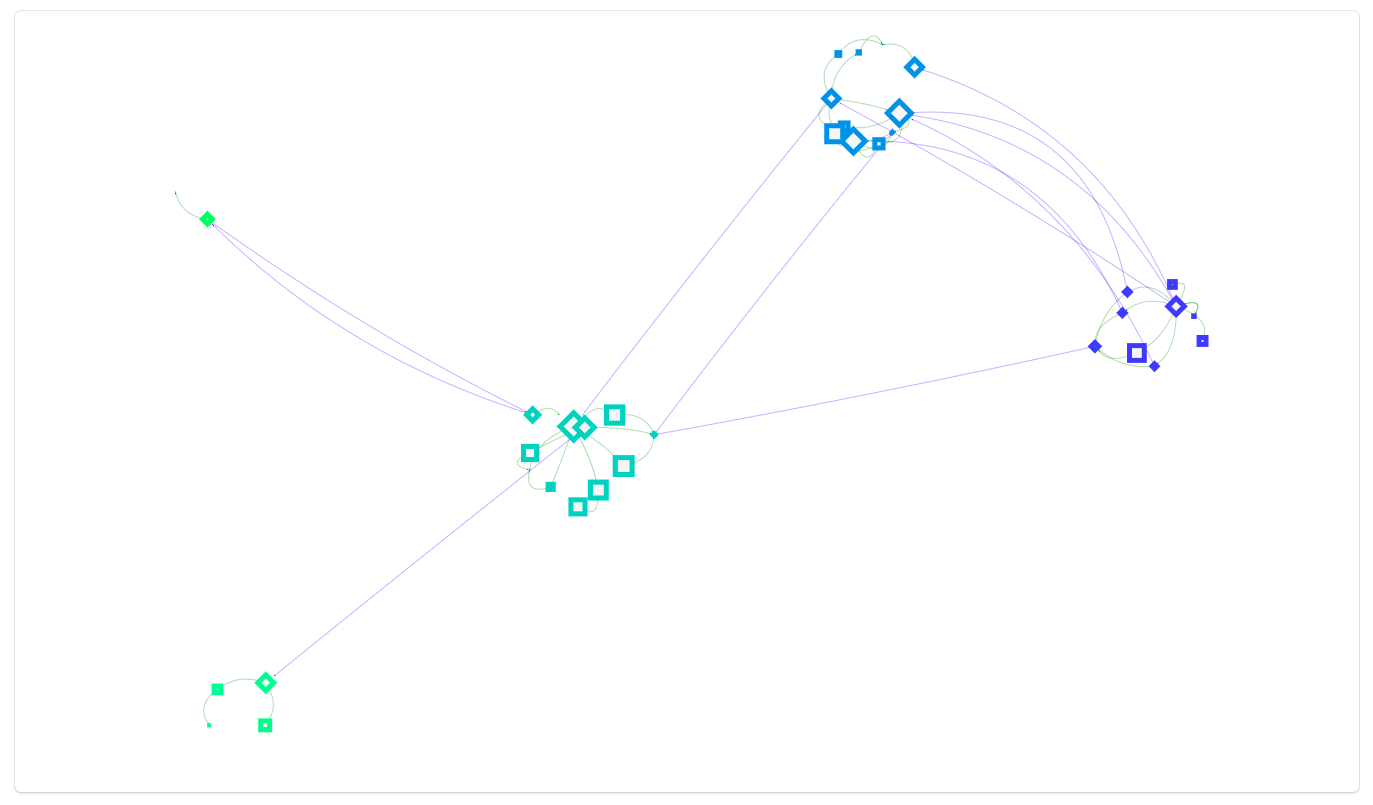
\includegraphics[width=.96\textwidth]{detailed-graph-view}
\caption{A closeup of the detailed graph view mode}
\caption*{\centering
  The graph view has a second, more detailed mode that also displays
  all of the inter-cluster as well as intra-cluster edges.
}
\label{fig:detailed-graph-view}
\end{figure}

\paragraph{Natural mode}
A last, additional graph view mode renders the graph in a more natural form
without artificial changes to the way that the clusters are rendered.
This mode is mainly interesting to examine the structure or architecture
of the input monolithic application.
The mode can be seen in figure \ref{fig:natural-graph-view} and is
activated by toggling the \textit{Clustered View} option which also disables
the \textit{Hide Inter-Cluster Edges} as well.

\begin{figure}[htbp]
\centering
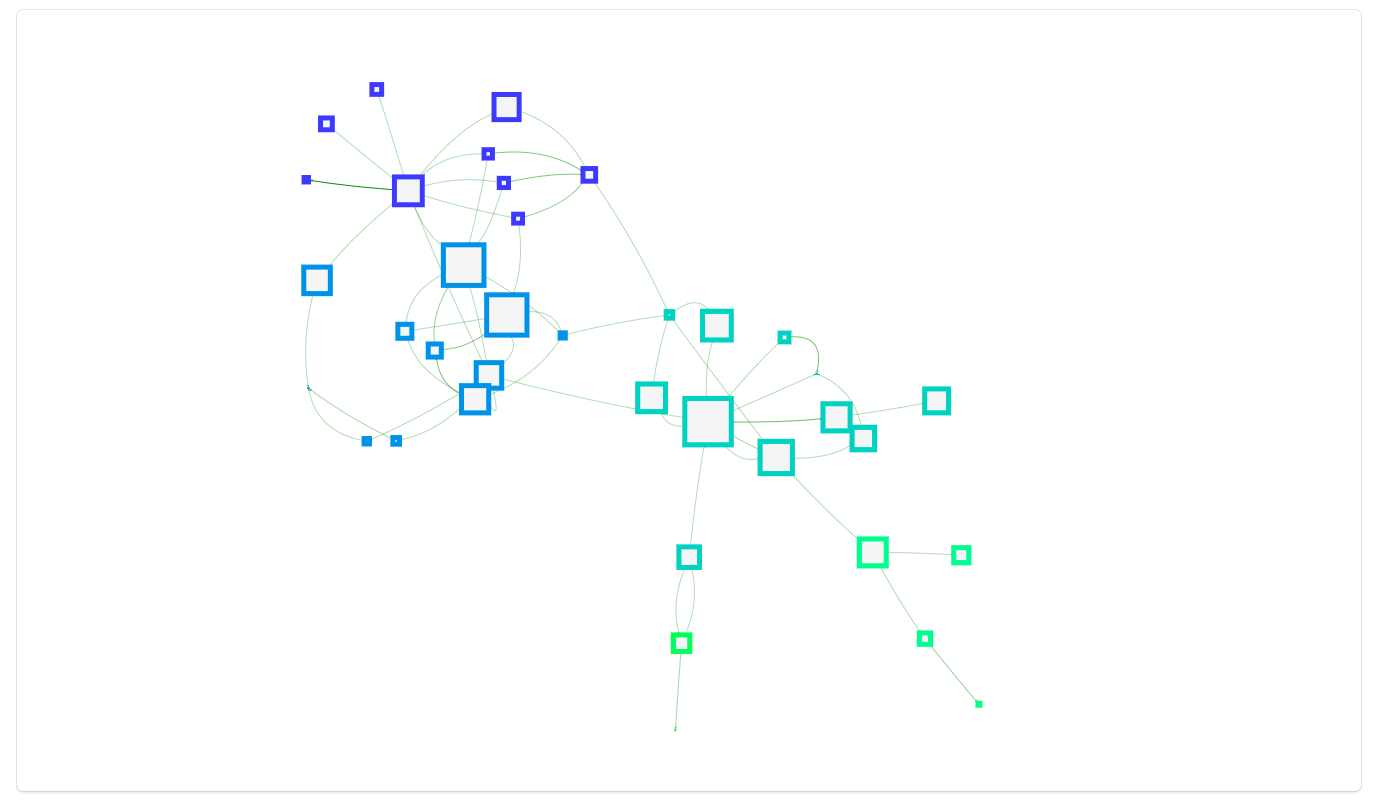
\includegraphics[width=.96\textwidth]{natural-graph-view}
\caption{A closeup of the natural graph view mode}
\caption*{\centering
  The \textit{graph view} has a third mode that can be used to see a more
  natural rendering of the clustered graph. This can be used to examine
  the structure of the input monolithic application on its own.
}
\label{fig:natural-graph-view}
\end{figure}


\subsubsection{Textual view}
As large input monolithic applications will also produce large graph clusterings,
the readability of the \textit{graph view} is hindered.
However especially when the microservice recommendations should
be implemented, a textual view is preferred as the graphical nature of the
\textit{graph view} is expected to not provide enough of an overview regarding
the resulting microservice candidate recommendations.
This view can be seen in further detail in figure \ref{fig:textual-view-ui}.

\begin{figure}[htbp]
\centering
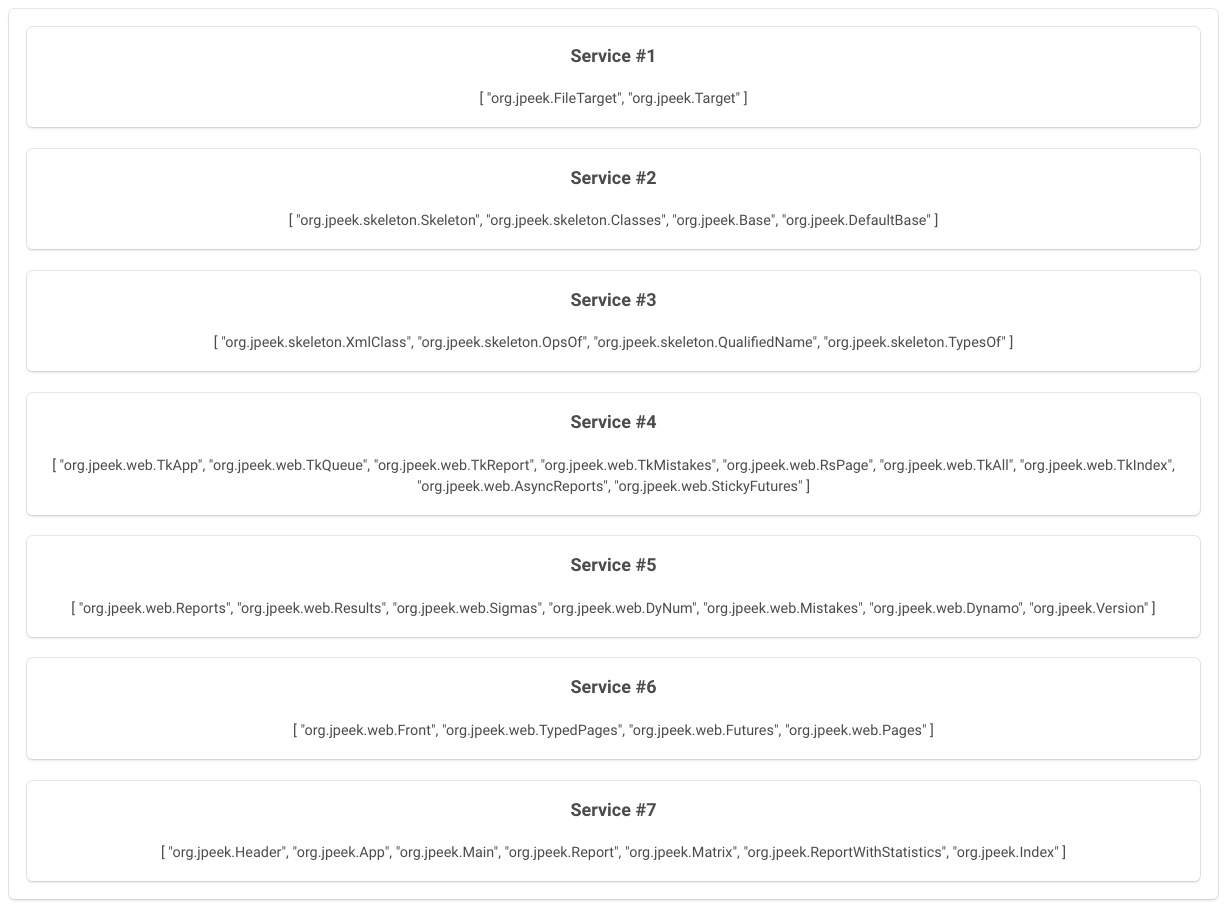
\includegraphics[width=.96\textwidth]{textual-view-ui}
\caption{A closeup of the textual view}
\caption*{\centering
  Additionally to the \textit{graph view}, a solely \textit{textual view}
  was implemented that just displays which units belong to which service.
}
\label{fig:textual-view-ui}
\end{figure}


\subsubsection{Metrics view}
Lastly, the UI displays an overview of the metrics that we selected.
All of those are covered in detail in chapter \ref{chap:metrics}.
The big tile on top of the others, as seen in figure \ref{fig:metrics-view-ui},
contains general metrics that are not measuring anything regarding the
clustering but rather the input.

\begin{figure}[htbp]
\centering
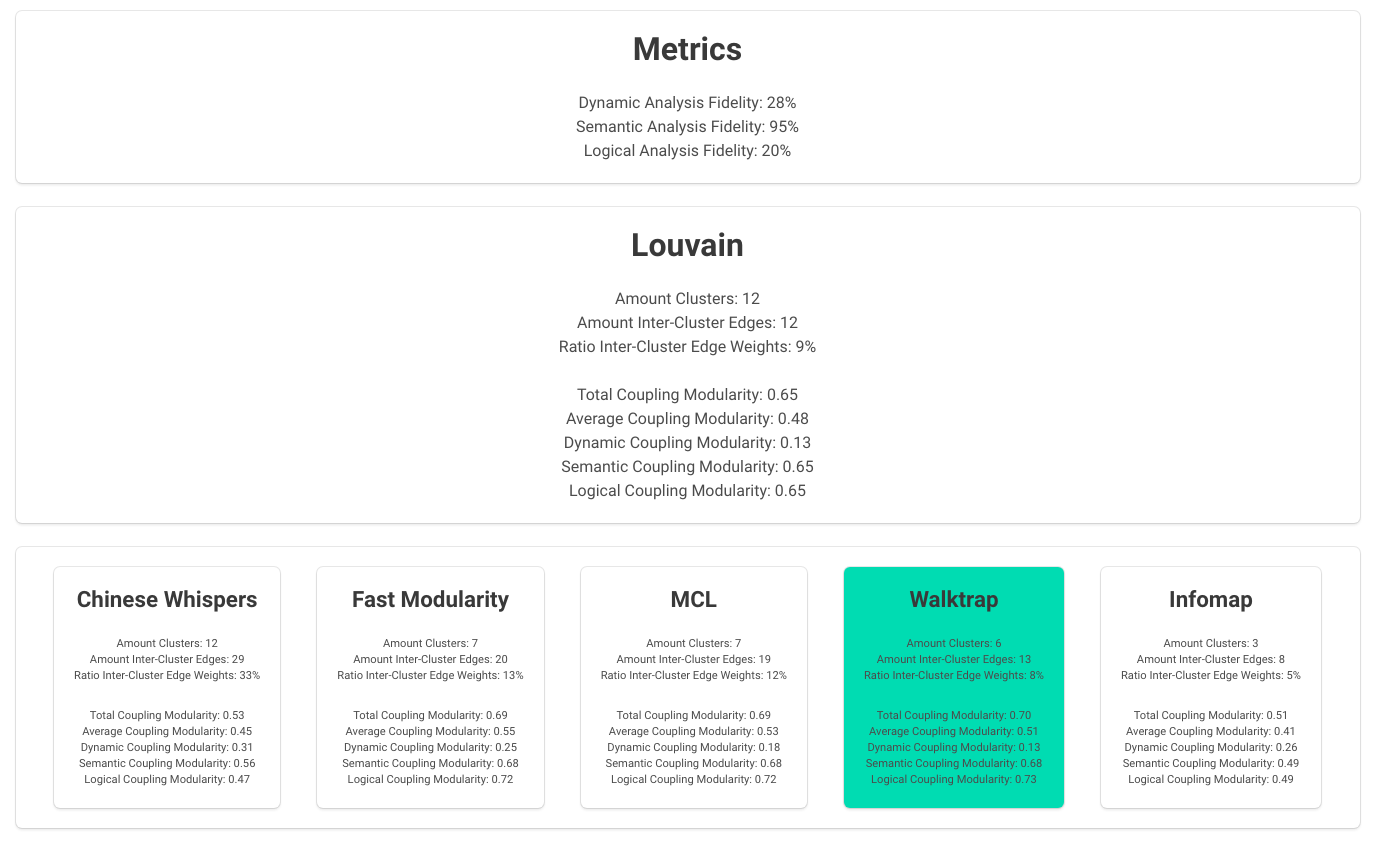
\includegraphics[width=\textwidth]{metrics-view-ui}
\caption{A closeup of the metrics view}
\caption*{\centering
  Every available graph clustering algorithm is evaluated while the one that
  scored the highest in the selected metric is additionally highlighted in green.
}
\label{fig:metrics-view-ui}
\end{figure}

The tile directly below is displaying results regarding the selected
graph clustering algorithm. However, the information is identical with the
smaller tiles below. Each tile corresponds to one of the available algorithms,
the selected one just gets the largest tile for better visibility.

Finally, the algorithm that scored the highest in the metric that was selected
in the third tile, next to the selected algorithm, is highlighted in green.




\chapter{Experiment design} \label{chap:experiment-design}

Our full implementation exhibited in chapter \ref{chap:implementation} allowed us
to evaluate our methodology using actual software which was selected via the
definition of a multitude of criteria followed by extensive research to identify
possible candidates for the experiments.



\section{Experiment setup}

Five freely available open-source applications as well as a closed source one
provided by the host organization of this thesis project were chosen to be run through
\textit{Steinmetz} to generate a set of microservice candidate recommendations.
The goal is to determine which graph clustering algorithm performed the best in the case
of each input application as well as overall.


\subsection{Subjects}

As shown in section \ref{sect:background-architecture}, a microservices\hyp based
architecture only makes sense for large\hyp scale, web\hyp based, back\hyp end
applications compared to libraries, SDKs, and dedicated GUI software.
Consequently, software that falls into said category had to be selected which
is far more difficult compared to the other categories as such software is
typically found in enterprises and not overly common in the open-source sector.

Additionally, the selected applications had to be implemented with the Java
programming language as the first version of \textit{Steinmetz} that we implemented
for now only supports input software that was written in Java.

Furthermore, to be able to analyze all three of the input dimensions covered in
section \ref{sect:software-quality-metrics}, the selected applications had to fulfill
another, more distinct set of criteria:

\begin{itemize}[noitemsep]
    \item Dynamic coupling: Executable in the latest version
    \item Semantic coupling: Being available as uncompiled source code
    \item Evolutionary coupling: Being version-controlled via a supported VCS
\end{itemize}

Based on these basic criteria, we conducted an intensive survey of possible ones
via the search functionality of GitHub. Precisely, these projects were found via
the following query \ref{github-query}.

\begin{lstlisting}[caption=GitHub experiment subjects search query, label=github-query, breaklines=true, basicstyle=\scriptsize\ttfamily]
NOT library NOT framework NOT distributed NOT client NOT android stars:>500 language:Java
\end{lstlisting}

Sadly, the GitHub search only allows up to five \code{NOT} operators.
Thus, this query still yields good results overall but still a lot of false positives such as:

\begin{itemize}[noitemsep]
    \item Libraries or SDKs not filtered out by the query
    \item Chinese repositories with unknown contents
    \item Collections of example code or interview questions
\end{itemize}

After discarding these, the first 50 pages of the search results were anaylyzed
for software projects of varying sizes with the following properties:

\begin{itemize}[noitemsep]
    \item standalone
    \item large\hyp scale
    \item web\hyp based
    \item back\hyp end
    \item monolithic
\end{itemize}

Finally, the six applications seen in table \ref{table:evaluation-projects}
that fulfill these requirements were selected.
Additionally, we added the major back-end application of the host organization
of this thesis which cannot be found on GitHub directly as its source is closed.

\begin{table}[ht!]
\def\arraystretch{1.55}
\begin{tabularx}{\textwidth}{|c|c|c|X|}
\hline
Project & Project Page & SLOC & Description \\
\hline\hline

Apache Solr     & \href{https://github.com/apache/lucene-solr}{GitHub Repository} & $203365$ &
A high-performance, fully\hyp featured text search engine \\\hline

Google Bazel    & \href{https://github.com/bazelbuild/bazel}{GitHub Repository} & $337292$ &
A fast, scalable, multi-language and extensible build system \\\hline

Heritrix        & \href{https://github.com/internetarchive/heritrix3}{GitHub Repository} & $15454$ &
The \textit{Internet Archive's} open-source, extensible, web-scale, archival-quality web
crawler project \\\hline

Picnic Store & \textit{Closed Source} & $26953$ &
The store back-end of \textit{Picnic} (the host organization of this thesis project) \\\hline

Teammates       & \href{https://github.com/TEAMMATES/teammates}{GitHub Repository} & $42280$ &
An online tool for managing peer evaluations and other feedback paths of students \\\hline

XWiki           & \href{https://github.com/xwiki/xwiki-platform}{GitHub Repository} & $231349$ &
An advanced open source enterprise wiki \\\hline

\end{tabularx}
\caption{The software projects selected for the evaluation}
\label{table:evaluation-projects}
\end{table}


\subsection{Difficulties} \label{subsect:difficulties}

As discussed in the previous section, the selected applications have to fulfill
a set of requirements for each of the three input dimensions.
Furthermore, the \textit{dynamic coupling} involves another difficulty which
was already discussed in subsection \ref{subsect:background-dynamic-analysis} ---
owing to the fact that the software has to be executed in order to conduct
\textit{dynamic program analysis}, this input dimension involves a lot more work
than any of the other.

Moreover, another problem arises which is more specific to
our use case: The dynamic coupling between units of the application that should
later belong to different microservices only becomes apparent while the application
is under full load by a real user base.
Otherwise, \textit{dynamic coupling} will be measured while it is easy to see
that the results are flawed when not analyzing actual load on the system.

This problem is actually twofold. Firstly, the coupling of non-production workload
is usually completely different from workload generated by an actual user base and
secondly, it is unlikely that most parts of the application will even be invoked.
One set of metrics that we devised that measure the \textit{fidelity} of the
different analysis types is useful to determine how severe this latter problem is.
However, the first problem is a dilemma as it just cannot be known how well the
workload during the \textit{dynamic analysis} resembled the \textit{dynamic coupling}
of the application when not conducted in a production environment.

Although load testing and example work loads exist, the recordings will still
not reach the quality of ones recorded in a running production environment.
Apart from the fact that even example workloads are very sparse for open-source
software, a production environment is simply not available to us to guarantee
high quality and high fidelity \textit{dynamic analysis}.
Overall, this is specifically problematic as some \textit{dynamic coupling} will always
be recorded which will in turn also be used to generate the microservice candidate
recommendations which are ergo flawed and unreliable.

Due to this difficulty and its possible repercussions, we decided to leave the
\textit{dynamic coupling} dimension out of most of the experiments.
Nevertheless, owing to the fact that our implementation allows for one input dimension
to be left out when conducting an analysis, this difficulty could be circumvented
during the first experiment.

Finally, to test that the entirety of our implemented methodology was working as designed,
we conducted the first experiment by analyzing one of the projects with all the available
dimensions, thus including the \textit{dynamic coupling}. The details of this first as
well as the others experiments are discussed in more detail in the following section
\ref{sect:experiment-execution}.



\section{Experiment execution} \label{sect:experiment-execution}

Before the actual experiments are exhibited, the criteria of each experiment are discussed
and explained. Table \ref{table:experiment-criteria} shows the five selected criteria that
every of the following experiments sets.

\begin{table}[ht!]
\def\arraystretch{1.55}
\begin{tabularx}{\textwidth}{|c|X|}
\hline
Criterion & Explanation \\
\hline\hline

Coupling dimensions            & The coupling dimensions that were used for the analysis (see \ref{sect:software-quality-metrics}) \\\hline

Coupling dimension weights     & The weights that were assigned to each of the utilized dimensions (see \ref{sect:merging-graphs}) \\\hline

Graph clustering algorithms     & The graph clustering algorithms that were used for the experiment (see \ref{sect:background-graph-clustering}) \\\hline

Maximum amount of iterations    & The maximum amount of iterations used for algorithms that require an input parameter (see \ref{graph-clustering-algorithm-survey-amount-of-clusters}) \\\hline

Recorded metrics                & The metrics that were recorded as part of the experiment (see \ref{chap:metrics}) \\\hline

\end{tabularx}
\caption{Explanations of the criteria of the experiments}
\label{table:experiment-criteria}
\end{table}


\subsection{Experiments}

\subsubsection{Experiment Nº 1}
For the first experiment, we analyzed only the test subject \textit{Heritrix} with
all available dimensions. The reason for this is that due to the nature of
\textit{Heritrix} it is feasible to record real\hyp world workload regarding the
\textit{dynamic coupling}. \textit{Heritrix} is a web\hyp crawler which means that
after being given one or multiple seeds, it generates its work automatically by
adding newly found links to a queue. Consequently, no workload has to be
synthetically generated or recorded which means that the problem discussed in
subsection \ref{subsect:difficulties} can be circumvented in this way.
Eventually, we profiled \textit{Heritrix} during its runtime for 48 hours with the
\textit{Java Flight Recorder} which yielded a recording of over 200 megabytes
which was used for this experiment.
Importantly, this is a proof of concept experiment as we acknowledge that its
results could be more meaningful with a larger set of test subjects.
Additionally, the \textit{coupling dimension weights} were set to different values.
These values were set by running the hyper\hyp parameter optimization detailed in
\ref{subsubsect:hyper-parameter-optimization} to maximize the
\textit{Average Mean Cluster Factor} metric.
Finally, the following criteria were determined:
\begin{itemize}[noitemsep]
    \item Coupling dimensions: dynamic, semantic, evolutionary
    \item Coupling dimension weights: $4 \times dynamic$, $4 \times semantic$, $7 \times evolutionary$
    \item Graph clustering algorithms: Chinese Whispers, Clauset-Newman-Moore, Infomap, Label Propagation, Louvain, MCL, Walktrap
    \item Maximum amount of iterations: 100
    \item Recorded metrics: \textit{Average Mean Cluster Factor}
\end{itemize}


\subsubsection{Experiment Nº 2}
For the second experiment, we analyzed all of the aforementioned test subjects
with our implementation. In essence, the criteria of this experiment are the
same as the one of the first one while the \textit{dynamic coupling} dimension
is left out due to the reasons described in subsection \ref{subsect:difficulties}:
\begin{itemize}[noitemsep]
    \item Coupling dimensions: semantic, evolutionary
    \item Coupling dimension weights: $1 \times semantic$, $1 \times evolutionary$
    \item Graph clustering algorithms: Chinese Whispers, Clauset-Newman-Moore, Infomap, Label Propagation, Louvain, MCL, Walktrap
    \item Maximum amount of iterations: 100
    \item Recorded metrics: \textit{Average Mean Cluster Factor},
    \textit{Amount of Clusters},
    \textit{Ratio Inter-Cluster Edge Weights}
\end{itemize}


\subsubsection{Experiment Nº 3}
In this third and hindmost experiment we recorded the average of each metric per graph
clustering algorithm with the intent to detect which ones generally perform
overly good or bad:
\begin{itemize}[noitemsep]
    \item Coupling dimensions: semantic, evolutionary
    \item Coupling dimension weights: $1 \times semantic$, $1 \times evolutionary$
    \item Graph clustering algorithms: Chinese Whispers, Clauset-Newman-Moore, Infomap, Label Propagation, Louvain, MCL, Walktrap
    \item Maximum amount of iterations: 100
    \item Recorded metrics: Average of \textit{Average Mean Cluster Factor} per algorithm,
    Average of \textit{Coefficient of variation of Average Mean Cluster Factor} per algorithm,
    Average of \textit{Amount of Clusters} per algorithm,
    Average of \textit{Ratio Inter-Cluster Edge Weights} per algorithm
\end{itemize}




\chapter{Evaluation} \label{chap:evaluation}

\section{Experiment Nº 1}

The results of experiment Nº 1 can be found in figures
\ref{fig:experiment-1.1}, \ref{fig:experiment-1.2}, \ref{fig:experiment-1.3}.

Generally, it can be quickly observed that the \textit{Dynamic Mean Cluster Factor}
values of most algorithms are fairly low.
We attribute this partly to the fact that the fidelity of the dynamic analysis
was rather low with $16\%$. Nevertheless, this experiment shows that our methodology
definitely works better on the other two input dimensions.

Apart from the \textit{Chinese Whispers} and \textit{Label Propagation} algorithms,
all other algorithms perform similarly achieving \textit{Average Mean Cluster Factor}
recordings around the mark of $60$.

The last interesting key point is that the algorithms scored fairly different
values for the metrics \textit{Amount of Clusters} and
\textit{Ratio Inter-Cluster Edge Weights} while reaching very similar
\textit{Average Mean Cluster Factor} scores, as just mentioned.
Specifically the \textit{Infomap} algorithm stands out with only $6$ clusters
and $2 \%$ of inter-cluster edge weights while achieving the highest
\textit{Average Mean Cluster Factor} score which can be mainly attributed to
its great overall performance in the \textit{Dynamic Mean Cluster Factor} metric
where most other algorithms did not score well.

\begin{figure}[p]
    \centering
    \begin{adjustbox}{width=\textwidth}
    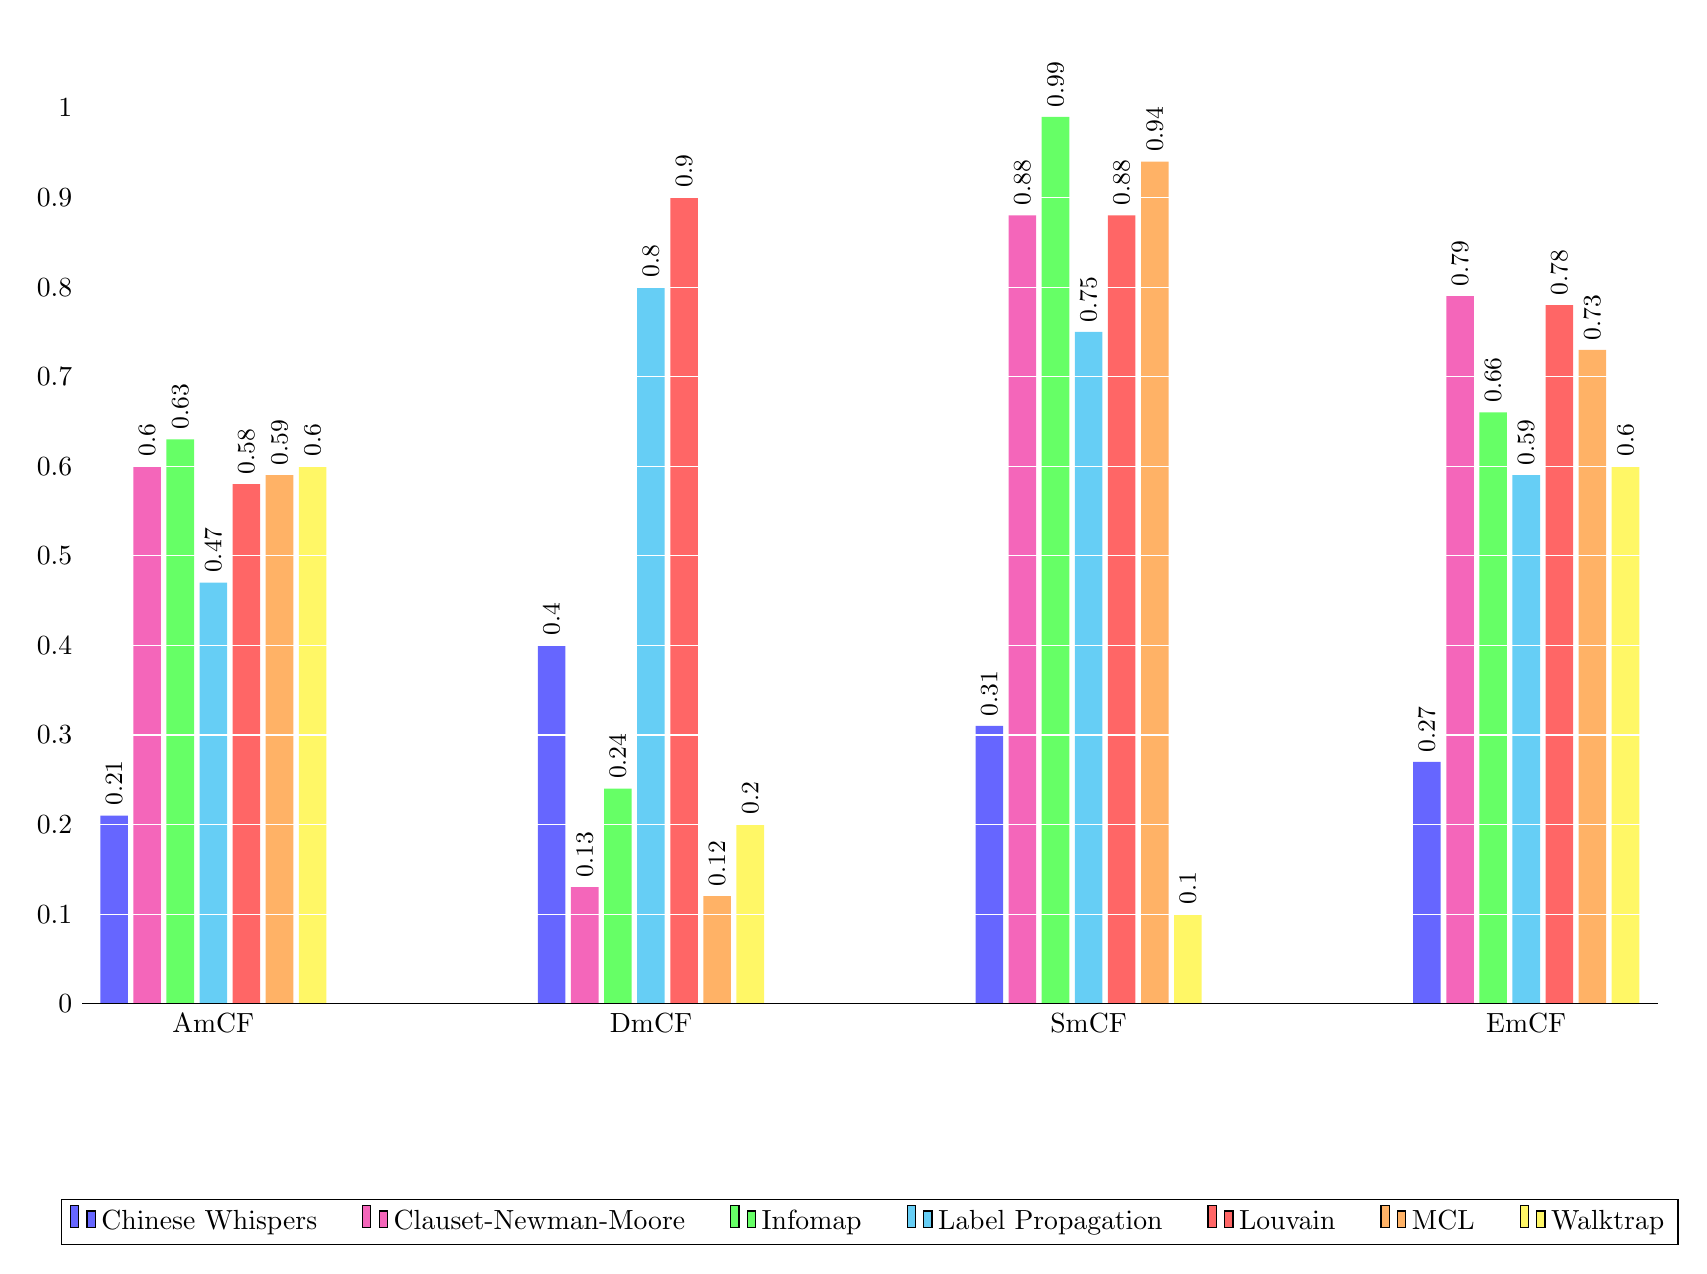
\begin{tikzpicture}
    \centering
    \begin{axis}[
        ybar, axis on top,
        height=\paperheight/2, width=\paperwidth,
        bar width=0.35cm,
        ymajorgrids, tick align=inside,
        major grid style={draw=white},
        enlarge y limits={value=.1,upper},
        ymin=0,
        axis x line*=bottom,
        axis y line*=left,
        y axis line style={opacity=0},
        tickwidth=0pt,
        enlarge x limits=true,
        legend style={
            at={(0.5,-0.2)},
            anchor=north,
            legend columns=-1,
            /tikz/every even column/.append style={column sep=0.5cm}
        },
        ylabel={},
        symbolic x coords={
          AmCF, % Average Mean Cluster Factor
          DmCF, % Dynamic Mean Cluster Factor
          SmCF, % Semantic Mean Cluster Factor
          EmCF, % Evolutionary Mean Cluster Factor
        },
        xtick=data,
        nodes near coords={
            \rot{\small{\pgfmathprintnumber[precision=2]{\pgfplotspointmeta}}}
        }
    ]
    % Chinese Whispers
    \addplot [draw=none, fill=blue!60] coordinates {
      (AmCF,0.21)
      (DmCF,0.4)
      (SmCF,0.31)
      (EmCF,0.27)
    };
    % Clauset-Newman-Moore
    \addplot [draw=none, fill=magenta!60] coordinates {
      (AmCF,0.60)
      (DmCF,0.13)
      (SmCF,0.88)
      (EmCF,0.79)
    };
    % Infomap
    \addplot [draw=none, fill=green!60] coordinates {
      (AmCF,0.63)
      (DmCF,0.24)
      (SmCF,0.99)
      (EmCF,0.66)
    };
    % Label Propagation
    \addplot [draw=none, fill=cyan!60] coordinates {
      (AmCF,0.47)
      (DmCF,0.8)
      (SmCF,0.75)
      (EmCF,0.59)
    };
    % Louvain
    \addplot [draw=none, fill=red!60] coordinates {
      (AmCF,0.58)
      (DmCF,0.9)
      (SmCF,0.88)
      (EmCF,0.78)
    };
    % MCL
    \addplot [draw=none, fill=orange!60] coordinates {
      (AmCF,0.59)
      (DmCF,0.12)
      (SmCF,0.94)
      (EmCF,0.73)
    };
    % Walktrap
    \addplot [draw=none, fill=yellow!60] coordinates {
      (AmCF,0.60)
      (DmCF,0.20)
      (SmCF,0.100)
      (EmCF,0.60)
    };
    \legend{Chinese Whispers,Clauset-Newman-Moore,Infomap,Label Propagation,Louvain,MCL,Walktrap}
    \end{axis}
\end{tikzpicture}
\end{adjustbox}
\caption{
  Plotted results of experiment Nº 1 (Part 1)
}
\caption*{\centering
  The labels represent the following metrics:
  \begin{itemize}[noitemsep]
    \item AmCF: Average Median Cluster Factor
    \item DmCF: Dynamic Median Cluster Factor
    \item SmCF: Semantic Median Cluster Factor
    \item EmCF: Evolutionary Median Cluster Factor
  \end{itemize}
}
\label{fig:experiment-1.1}
\end{figure}

\begin{figure}[p]
    \centering
    \begin{adjustbox}{width=\textwidth}
    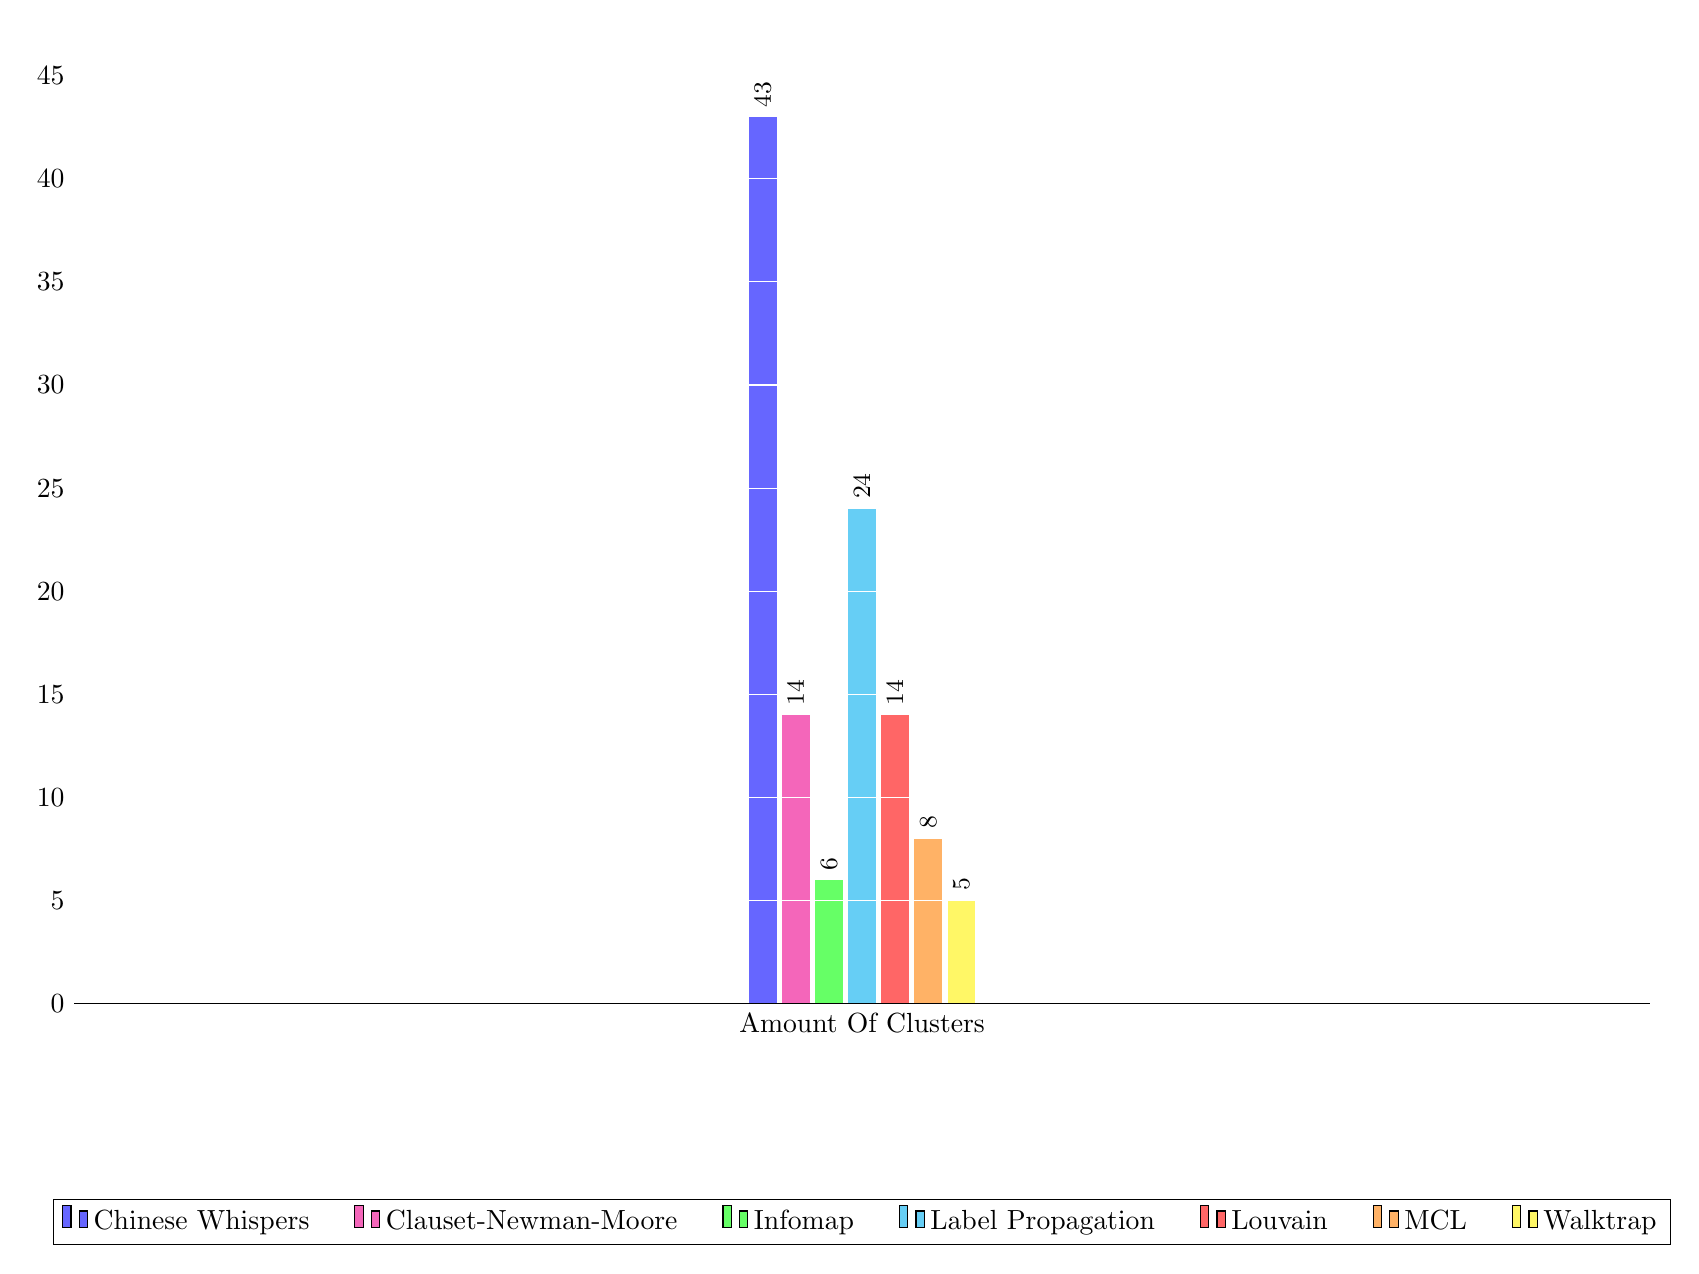
\begin{tikzpicture}
    \centering
    \begin{axis}[
        ybar, axis on top,
        height=\paperheight/2, width=\paperwidth,
        bar width=0.35cm,
        ymajorgrids, tick align=inside,
        major grid style={draw=white},
        enlarge y limits={value=.1,upper},
        ymin=0,
        axis x line*=bottom,
        axis y line*=left,
        y axis line style={opacity=0},
        tickwidth=0pt,
        enlarge x limits=true,
        legend style={
            at={(0.5,-0.2)},
            anchor=north,
            legend columns=-1,
            /tikz/every even column/.append style={column sep=0.5cm}
        },
        ylabel={},
        symbolic x coords={
          Amount Of Clusters
        },
        xtick=data,
        nodes near coords={
            \rot{\small{\pgfmathprintnumber[precision=1]{\pgfplotspointmeta}}}
        }
    ]
    % Chinese Whispers
    \addplot [draw=none, fill=blue!60] coordinates {
      (Amount Of Clusters,43)
    };
    % Clauset-Newman-Moore
    \addplot [draw=none, fill=magenta!60] coordinates {
      (Amount Of Clusters,14)
    };
    % Infomap
    \addplot [draw=none, fill=green!60] coordinates {
      (Amount Of Clusters,6)
    };
    % Label Propagation
    \addplot [draw=none, fill=cyan!60] coordinates {
      (Amount Of Clusters,24)
    };
    % Louvain
    \addplot [draw=none, fill=red!60] coordinates {
      (Amount Of Clusters,14)
    };
    % MCL
    \addplot [draw=none, fill=orange!60] coordinates {
      (Amount Of Clusters,8)
    };
    % Walktrap
    \addplot [draw=none, fill=yellow!60] coordinates {
      (Amount Of Clusters,5)
    };
    \legend{Chinese Whispers,Clauset-Newman-Moore,Infomap,Label Propagation,Louvain,MCL,Walktrap}
    \end{axis}
\end{tikzpicture}
\end{adjustbox}
\caption{
  Plotted results of experiment Nº 1 (Part 2)
}
\label{fig:experiment-1.2}
\end{figure}

\begin{figure}[p]
    \centering
    \begin{adjustbox}{width=\textwidth}
    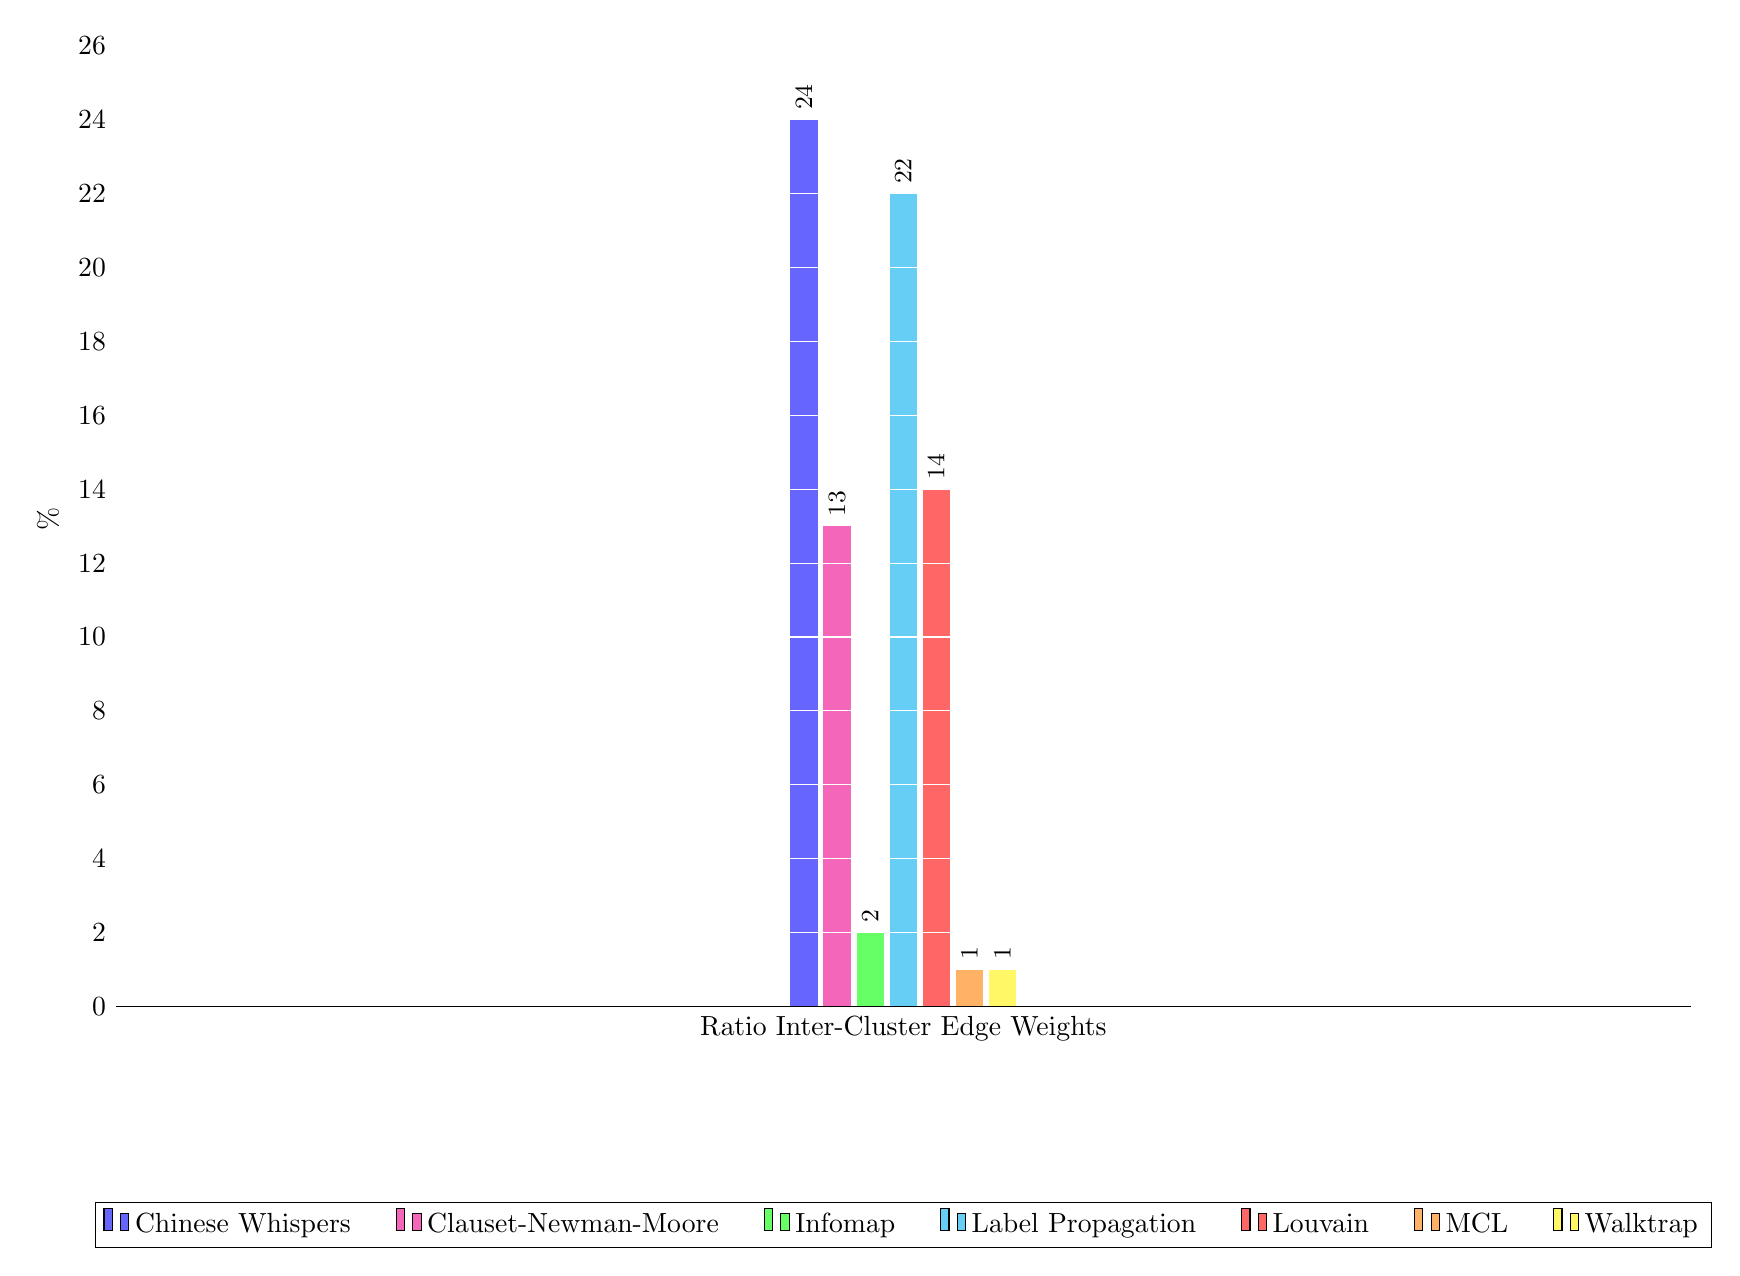
\begin{tikzpicture}
    \centering
    \begin{axis}[
        ybar, axis on top,
        height=\paperheight/2, width=\paperwidth,
        bar width=0.35cm,
        ymajorgrids, tick align=inside,
        major grid style={draw=white},
        enlarge y limits={value=.1,upper},
        ymin=0,
        axis x line*=bottom,
        axis y line*=left,
        y axis line style={opacity=0},
        tickwidth=0pt,
        enlarge x limits=true,
        legend style={
            at={(0.5,-0.2)},
            anchor=north,
            legend columns=-1,
            /tikz/every even column/.append style={column sep=0.5cm}
        },
        ylabel={\%},
        symbolic x coords={
          Ratio Inter-Cluster Edge Weights
        },
        xtick=data,
        nodes near coords={
            \rot{\small{\pgfmathprintnumber[precision=1]{\pgfplotspointmeta}}}
        }
    ]
    % Chinese Whispers
    \addplot [draw=none, fill=blue!60] coordinates {
      (Ratio Inter-Cluster Edge Weights,24)
    };
    % Clauset-Newman-Moore
    \addplot [draw=none, fill=magenta!60] coordinates {
      (Ratio Inter-Cluster Edge Weights,13)
    };
    % Infomap
    \addplot [draw=none, fill=green!60] coordinates {
      (Ratio Inter-Cluster Edge Weights,2)
    };
    % Label Propagation
    \addplot [draw=none, fill=cyan!60] coordinates {
      (Ratio Inter-Cluster Edge Weights,22)
    };
    % Louvain
    \addplot [draw=none, fill=red!60] coordinates {
      (Ratio Inter-Cluster Edge Weights,14)
    };
    % MCL
    \addplot [draw=none, fill=orange!60] coordinates {
      (Ratio Inter-Cluster Edge Weights,1)
    };
    % Walktrap
    \addplot [draw=none, fill=yellow!60] coordinates {
      (Ratio Inter-Cluster Edge Weights,1)
    };
    \legend{Chinese Whispers,Clauset-Newman-Moore,Infomap,Label Propagation,Louvain,MCL,Walktrap}
    \end{axis}
\end{tikzpicture}
\end{adjustbox}
\caption{
  Plotted results of experiment Nº 1 (Part 3)
}
\label{fig:experiment-1.3}
\end{figure}



\section{Experiment Nº 2}

The results of experiment Nº 2 can be found in figures \ref{fig:experiment-2.1},
\ref{fig:experiment-2.2}, and \ref{fig:experiment-2.3}.

It can be noticed quickly that the \textit{Chinese Whispers} algorithm performs
bad overall. Its performance is far worse than that of any other algorithm.
Furthermore, some algorithms perform better or worse on different projects,
while the \textit{Chinese Whispers} algorithm is consistently underperforming.
In the same vein, the \textit{Chinese Whispers} algorithm
stands out with yielding a grotesque amount of clusters --- which lead to
its low values in the \textit{Average Mean Cluster Factor} metric.
In the case of the test subjects \textit{Apache Solr} and \textit{Google Bazel},
it did not even fit into the figure anymore but clustered the projects into
$1348$ and $2100$ clusters respectively.
Consequently, the same is true for the last metric, \textit{Ratio Inter-Cluster Edge Weights},
where low values are better.

Additionally, it can be observed that the algorithms \textit{Clauset-Newman-Moore}
and \textit{Louvain} perform very similarly in all of the three recorded metrics,
which is due to the fact that they are both heuristic algorithms optimizing toward
the \textit{Modularity} metric \ref{subsect:renowned-graph-clustering-algorithms}.
Interestingly, in most occasions however, the \textit{Louvain} algorithm performs
slightly better which is a confirmation of the fact that it was developed after
the \textit{Clauset-Newman-Moore} algorithm and is seen as an improvement upon it
by literature \cite{lancichinetti2009community}.

Regarding the test subjects, we saw that generally projects with lower \textit{SLOC} counts
(i.e. smaller projects) could achieve better metric values and were easier to cluster
by all of the algorithms. This becomes specifially apparent for two of the larger
projects, \textit{Apache Solr} and \textit{Google Bazel}, which achieved lower
\textit{Average Mean Cluster Factor} values than all of the other test subjects.
The test subject \textit{XWiki} being the second largest in terms of \textit{SLOC} while
achieving good \textit{Average Mean Cluster Factor} values does not confirm the
theory that our methodology performs worse on larger input projects.
Additionally, we verified this conjecture by calculating the
\textit{Pearson correlation coefficient} \cite{everitt2002cambridge}
between the \textit{Average Mean Cluster Factor}
recordings and the \textit{SLOC} of the recorded test subject and the result is only
a slight negative correlation of \(r = -0.261\) --- meaning that when the \textit{SLOC} is
rising, the \textit{Average Mean Cluster Factor} is falling, albeit not in a meaningful manner.
Similarly, the correlation between the \textit{Amount of Clusters} and the \textit{SLOC}
of a test subject is not very indicative either with \(r = 0.363\).

Positively, apart from the \textit{Apache Solr} and \textit{Google Bazel} projects,
all other projects could be clustered into microservice recommendations with
solid metric results. Unfortunately, we have no explanation why these two projects
score so much worse compared to the others.

Finally, this was the only occasion that this ever happened during our experiments,
but the \textit{Walktrap} algorithm created only one cluster when clustering the
\textit{Teammates} project which is treated as an invalid result by us.


\begin{figure}[p]
    \centering
    \begin{adjustbox}{width=\textwidth}
    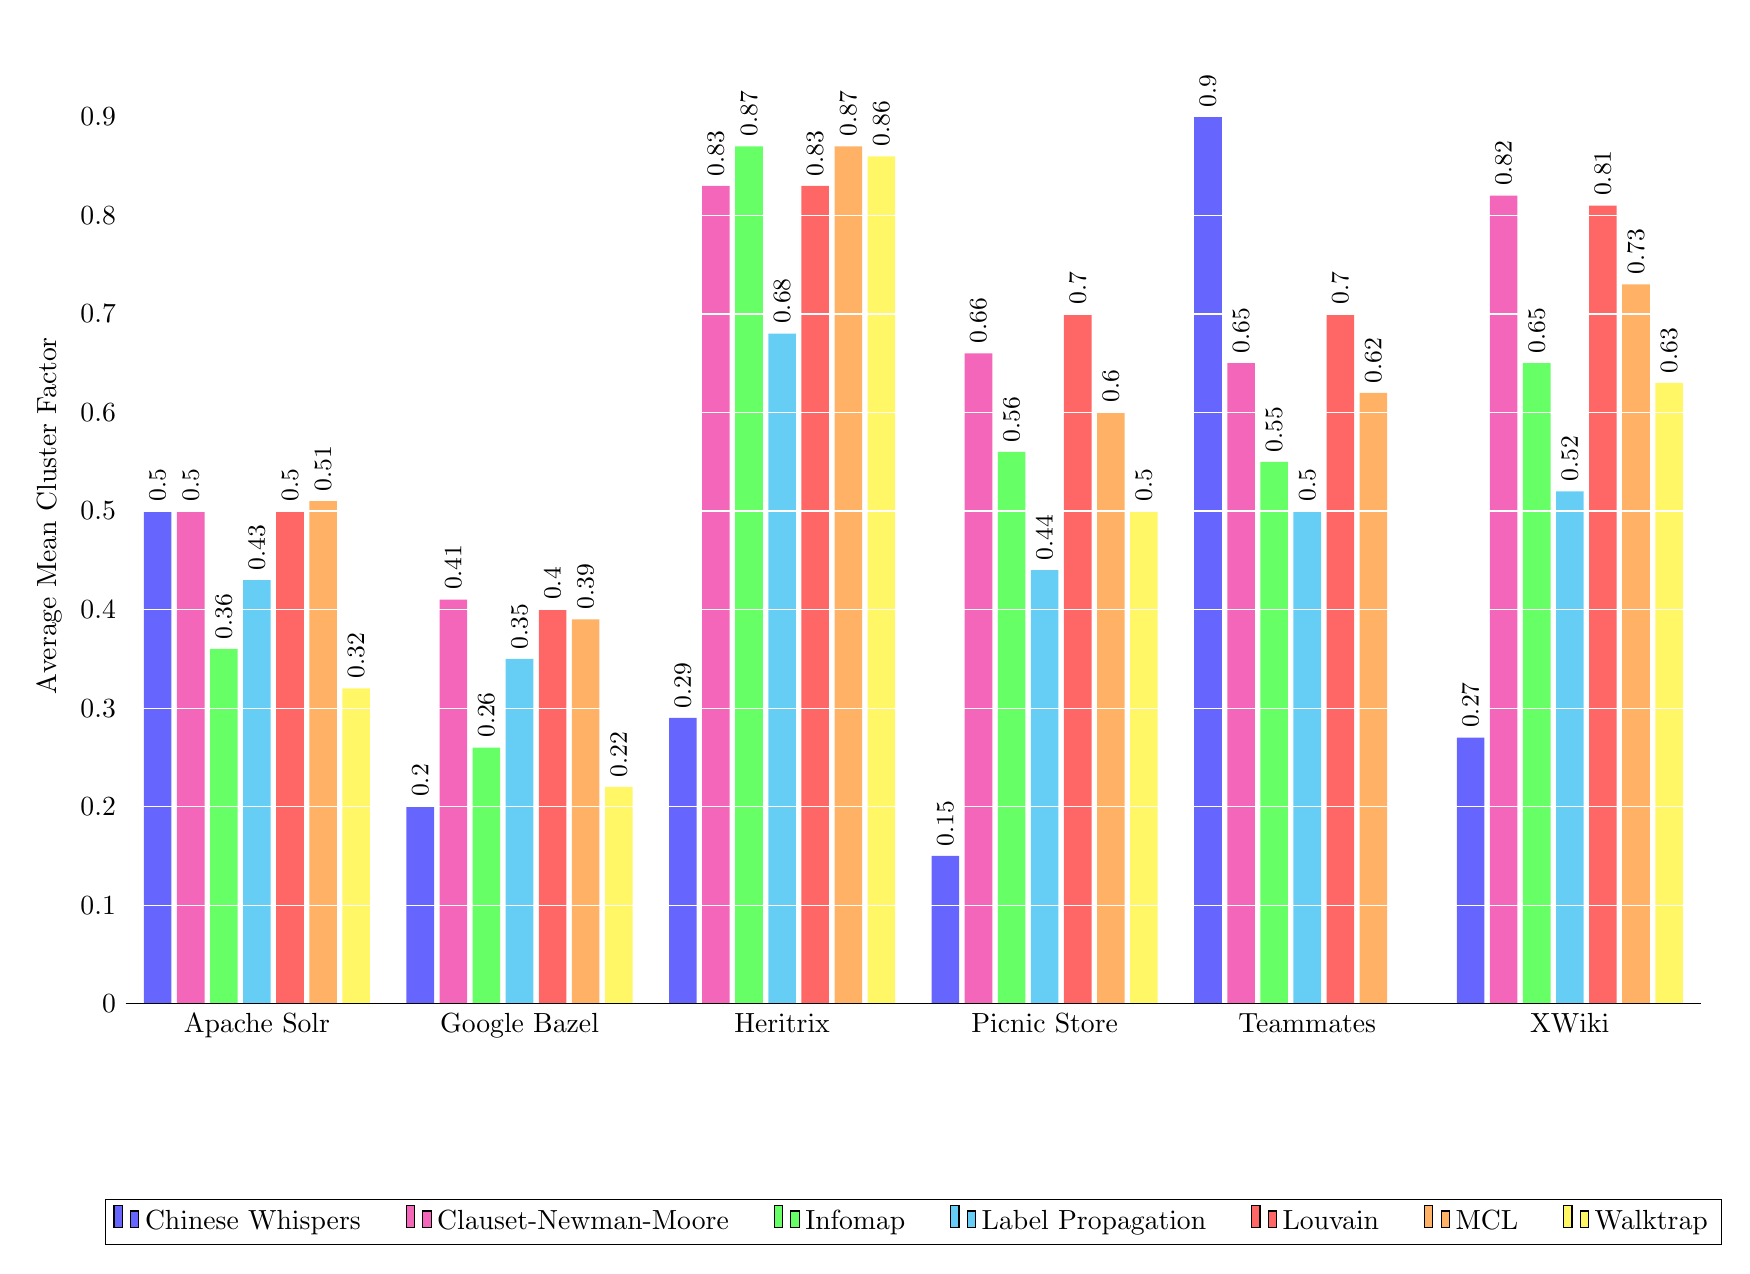
\begin{tikzpicture}
    \centering
    \begin{axis}[
        ybar, axis on top,
        height=\paperheight/2, width=\paperwidth,
        bar width=0.35cm,
        ymajorgrids, tick align=inside,
        major grid style={draw=white},
        enlarge y limits={value=.1,upper},
        ymin=0,
        axis x line*=bottom,
        axis y line*=left,
        y axis line style={opacity=0},
        tickwidth=0pt,
        enlarge x limits=true,
        legend style={
            at={(0.5,-0.2)},
            anchor=north,
            legend columns=-1,
            /tikz/every even column/.append style={column sep=0.5cm}
        },
        ylabel={Average Mean Cluster Factor},
        symbolic x coords={
          Apache Solr,
          Google Bazel,
          Heritrix,
          Picnic Store,
          Teammates,
          XWiki,
        },
        xtick=data,
        nodes near coords={
            \rot{\small{\pgfmathprintnumber[precision=2]{\pgfplotspointmeta}}}
        }
    ]
    % Chinese Whispers
    \addplot [draw=none, fill=blue!60] coordinates {
      (Apache Solr,0.5)
      (Google Bazel,0.2)
      (Heritrix,0.29)
      (Picnic Store,0.15)
      (Teammates,0.9)
      (XWiki,0.27)
    };
    % Clauset-Newman-Moore
    \addplot [draw=none, fill=magenta!60] coordinates {
      (Apache Solr,0.50)
      (Google Bazel,0.41)
      (Heritrix,0.83)
      (Picnic Store,0.66)
      (Teammates,0.65)
      (XWiki,0.82)
    };
    % Infomap
    \addplot [draw=none, fill=green!60] coordinates {
      (Apache Solr,0.36)
      (Google Bazel,0.26)
      (Heritrix,0.87)
      (Picnic Store,0.56)
      (Teammates,0.55)
      (XWiki,0.65)
    };
    % Label Propagation
    \addplot [draw=none, fill=cyan!60] coordinates {
      (Apache Solr,0.43)
      (Google Bazel,0.35)
      (Heritrix,0.68)
      (Picnic Store,0.44)
      (Teammates,0.50)
      (XWiki,0.52)
    };
    % Louvain
    \addplot [draw=none, fill=red!60] coordinates {
      (Apache Solr,0.50)
      (Google Bazel,0.40)
      (Heritrix,0.83)
      (Picnic Store,0.70)
      (Teammates,0.70)
      (XWiki,0.81)
    };
    % MCL
    \addplot [draw=none, fill=orange!60] coordinates {
      (Apache Solr,0.51)
      (Google Bazel,0.39)
      (Heritrix,0.87)
      (Picnic Store,0.60)
      (Teammates,0.62)
      (XWiki,0.73)
    };
    % Walktrap
    \addplot [draw=none, fill=yellow!60] coordinates {
      (Apache Solr,0.32)
      (Google Bazel,0.22)
      (Heritrix,0.86)
      (Picnic Store,0.50)
      (Teammates,nan)
      (XWiki,0.63)
    };
    \legend{Chinese Whispers,Clauset-Newman-Moore,Infomap,Label Propagation,Louvain,MCL,Walktrap}
    \end{axis}
\end{tikzpicture}
\end{adjustbox}
\caption{
  Plotted results of experiment Nº 2 (Part 1)
}
\label{fig:experiment-2.1}
\end{figure}

\begin{figure}[p]
    \centering
    \begin{adjustbox}{width=\textwidth}
    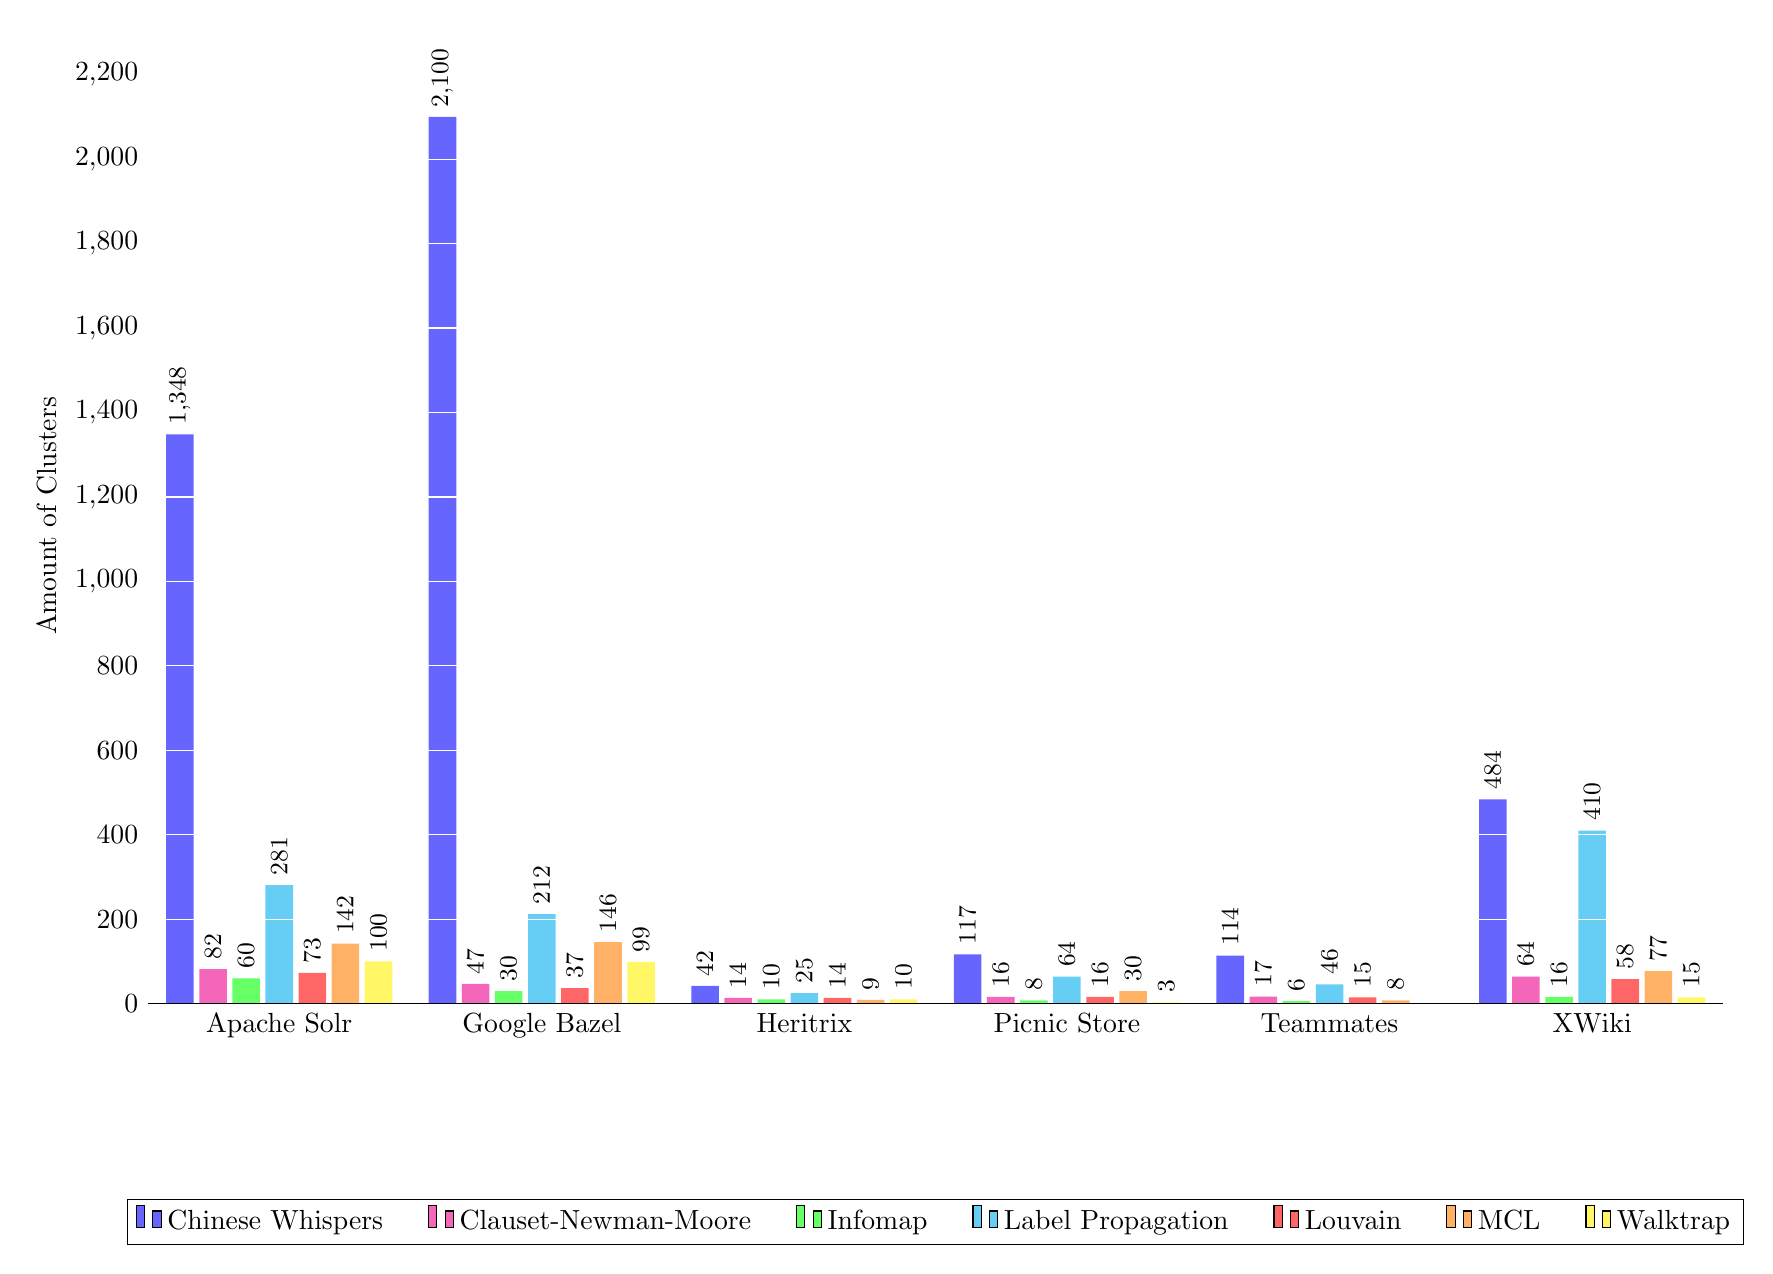
\begin{tikzpicture}
    \centering
    \begin{axis}[
        ybar, axis on top,
        height=\paperheight/2, width=\paperwidth,
        bar width=0.35cm,
        ymajorgrids, tick align=inside,
        major grid style={draw=white},
        enlarge y limits={value=.1,upper},
        ymin=0,
        axis x line*=bottom,
        axis y line*=left,
        y axis line style={opacity=0},
        tickwidth=0pt,
        enlarge x limits=true,
        legend style={
            at={(0.5,-0.2)},
            anchor=north,
            legend columns=-1,
            /tikz/every even column/.append style={column sep=0.5cm}
        },
        ylabel={Amount of Clusters},
        symbolic x coords={
          Apache Solr,
          Google Bazel,
          Heritrix,
          Picnic Store,
          Teammates,
          XWiki
        },
        xtick=data,
        nodes near coords={
            \rot{\small{\pgfmathprintnumber[precision=1]{\pgfplotspointmeta}}}
        }
    ]
    % Chinese Whispers
    \addplot [draw=none, fill=blue!60] coordinates {
      (Apache Solr,1348)
      (Google Bazel,2100)
      (Heritrix,42)
      (Picnic Store,117)
      (Teammates,114)
      (XWiki,484)
    };
    % Clauset-Newman-Moore
    \addplot [draw=none, fill=magenta!60] coordinates {
      (Apache Solr,82)
      (Google Bazel,47)
      (Heritrix,14)
      (Picnic Store,16)
      (Teammates,17)
      (XWiki,64)
    };
    % Infomap
    \addplot [draw=none, fill=green!60] coordinates {
      (Apache Solr,60)
      (Google Bazel,30)
      (Heritrix,10)
      (Picnic Store,8)
      (Teammates,6)
      (XWiki,16)
    };
    % Label Propagation
    \addplot [draw=none, fill=cyan!60] coordinates {
      (Apache Solr,281)
      (Google Bazel,212)
      (Heritrix,25)
      (Picnic Store,64)
      (Teammates,46)
      (XWiki,410)
    };
    % Louvain
    \addplot [draw=none, fill=red!60] coordinates {
      (Apache Solr,73)
      (Google Bazel,37)
      (Heritrix,14)
      (Picnic Store,16)
      (Teammates,15)
      (XWiki,58)
    };
    % MCL
    \addplot [draw=none, fill=orange!60] coordinates {
      (Apache Solr,142)
      (Google Bazel,146)
      (Heritrix,9)
      (Picnic Store,30)
      (Teammates,8)
      (XWiki,77)
    };
    % Walktrap
    \addplot [draw=none, fill=yellow!60] coordinates {
      (Apache Solr,100)
      (Google Bazel,99)
      (Heritrix,10)
      (Picnic Store,3)
      (Teammates,nan)
      (XWiki,15)
    };
    \legend{Chinese Whispers,Clauset-Newman-Moore,Infomap,Label Propagation,Louvain,MCL,Walktrap}
    \end{axis}
\end{tikzpicture}
\end{adjustbox}
\caption{
  Plotted results of experiment Nº 2 (Part 2)
}
\label{fig:experiment-2.2}
\end{figure}

\begin{figure}[p]
    \centering
    \begin{adjustbox}{width=\textwidth}
    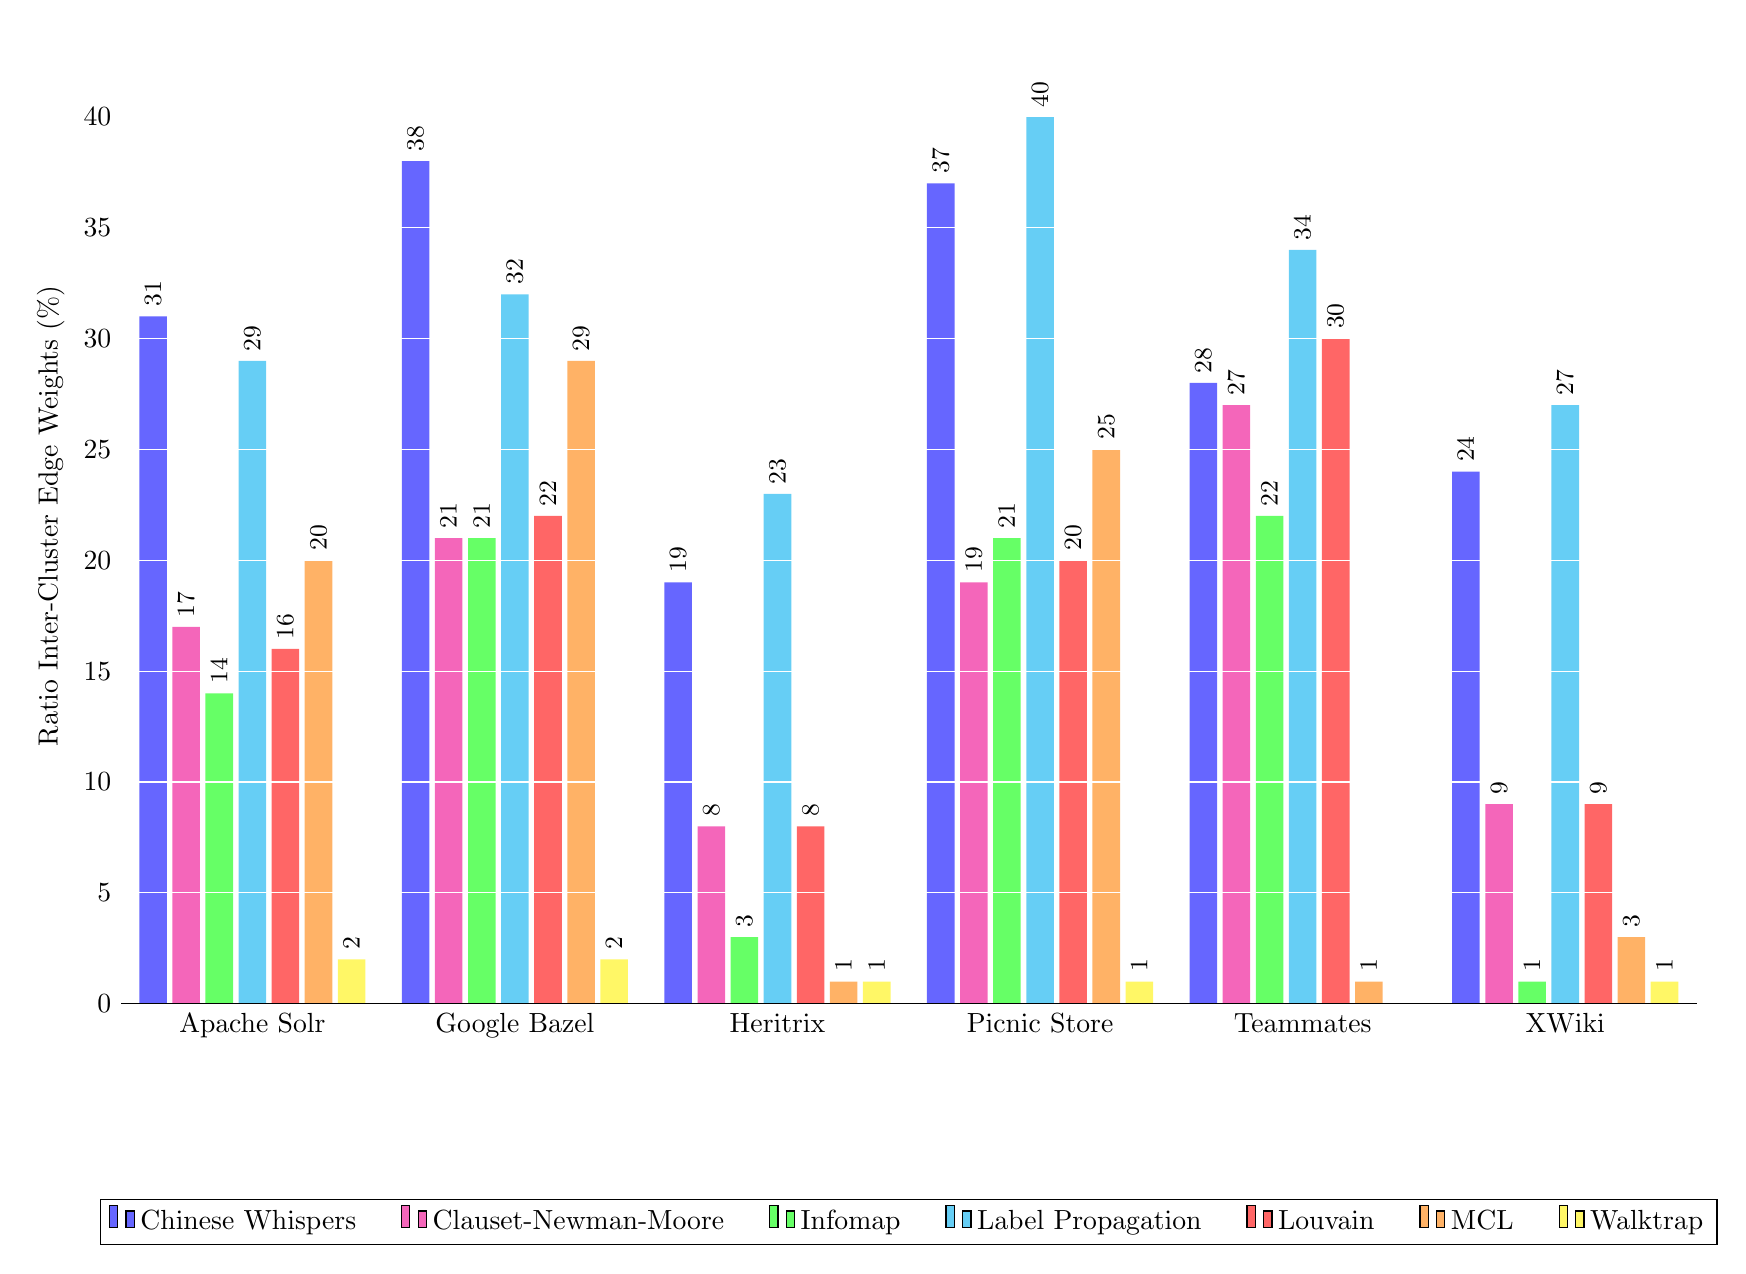
\begin{tikzpicture}
    \centering
    \begin{axis}[
        ybar, axis on top,
        height=\paperheight/2, width=\paperwidth,
        bar width=0.35cm,
        ymajorgrids, tick align=inside,
        major grid style={draw=white},
        enlarge y limits={value=.1,upper},
        ymin=0,
        axis x line*=bottom,
        axis y line*=left,
        y axis line style={opacity=0},
        tickwidth=0pt,
        enlarge x limits=true,
        legend style={
            at={(0.5,-0.2)},
            anchor=north,
            legend columns=-1,
            /tikz/every even column/.append style={column sep=0.5cm}
        },
        ylabel={Ratio Inter-Cluster Edge Weights (\%)},
        symbolic x coords={
          Apache Solr,
          Google Bazel,
          Heritrix,
          Picnic Store,
          Teammates,
          XWiki
        },
        xtick=data,
        nodes near coords={
            \rot{\small{\pgfmathprintnumber[precision=1]{\pgfplotspointmeta}}}
        }
    ]
    % Chinese Whispers
    \addplot [draw=none, fill=blue!60] coordinates {
      (Apache Solr,31)
      (Google Bazel,38)
      (Heritrix,19)
      (Picnic Store,37)
      (Teammates,28)
      (XWiki,24)
    };
    % Clauset-Newman-Moore
    \addplot [draw=none, fill=magenta!60] coordinates {
      (Apache Solr,17)
      (Google Bazel,21)
      (Heritrix,8)
      (Picnic Store,19)
      (Teammates,27)
      (XWiki,9)
    };
    % Infomap
    \addplot [draw=none, fill=green!60] coordinates {
      (Apache Solr,14)
      (Google Bazel,21)
      (Heritrix,3)
      (Picnic Store,21)
      (Teammates,22)
      (XWiki,1)
    };
    % Label Propagation
    \addplot [draw=none, fill=cyan!60] coordinates {
      (Apache Solr,29)
      (Google Bazel,32)
      (Heritrix,23)
      (Picnic Store,40)
      (Teammates,34)
      (XWiki,27)
    };
    % Louvain
    \addplot [draw=none, fill=red!60] coordinates {
      (Apache Solr,16)
      (Google Bazel,22)
      (Heritrix,8)
      (Picnic Store,20)
      (Teammates,30)
      (XWiki,9)
    };
    % MCL
    \addplot [draw=none, fill=orange!60] coordinates {
      (Apache Solr,20)
      (Google Bazel,29)
      (Heritrix,1)
      (Picnic Store,25)
      (Teammates,1)
      (XWiki,3)
    };
    % Walktrap
    \addplot [draw=none, fill=yellow!60] coordinates {
      (Apache Solr,2)
      (Google Bazel,2)
      (Heritrix,1)
      (Picnic Store,1)
      (Teammates,nan)
      (XWiki,1)
    };
    \legend{Chinese Whispers,Clauset-Newman-Moore,Infomap,Label Propagation,Louvain,MCL,Walktrap}
    \end{axis}
\end{tikzpicture}
\end{adjustbox}
\caption{
  Plotted results of experiment Nº 2 (Part 3)
}
\label{fig:experiment-2.3}
\end{figure}



\section{Experiment Nº 3}

The results of experiment Nº 3 can be found in figures
\ref{fig:experiment-3.1}, \ref{fig:experiment-3.2}, \ref{fig:experiment-3.3},
and \ref{fig:experiment-3.4}.

The \textit{Average of Amount of Clusters} is differing a lot, especially considering
that the \textit{Average of Average Mean Cluster Factor} and the
\textit{Average of Ratio Inter-Cluster Edge Weights} are fairly similar.
Specifically interesting is the case of the \textit{MCL} algorithm which yields
a lot of clusters on average while achieving the second best
\textit{Average of Ratio Inter-Cluster Edge Weights} and the third best
\textit{Average of Average Mean Cluster Factor} values.
This shows that the problem domain is filled with many local optima as different
algorithms can achieve good results with very divergent cluster amounts.

A similar case regarding the \textit{Average of Ratio Inter-Cluster Edge Weights}
goes for the \textit{Walktrap} algorithm who really stands out in that metric.
It scores good overall performance in the main
\textit{Average of Average Mean Cluster Factor} metric while recording only about
$1 \%$ of \textit{Average of Ratio Inter-Cluster Edge Weights}, an impressive value.

Additionally, the \textit{Average of Average Mean Cluster Factor} metrics were satisfactory
across\hyp the\hyp board, with a \textit{coefficient of variation}
\cite{everitt2002cambridge} of \(c_v = 33.9\) and even \(c_v = 11.1\) when leaving out
the distorting \textit{Chinese Whispers} algorithm.

Finally, the following two takeaways directly answer the third research question:
The first key point in this experiment is that the the \textit{Chinese Whispers},
\textit{Label Propagation}, and \textit{Walktrap} algorithms are performing the
worst overall and generally do not seem to be suitable for clustering graphs
representing software specifially when observing the recorded
\textit{Amount of Clusters} values which are irrationally
high with $700.83$ and $171.17$ respectively for the \textit{Chinese Whispers} and
\textit{Label Propagation} algorithms. The \textit{Walktrap} algorithm on the other
hand performs erraticly with a \textit{coefficient of variation} of \(c_v = 49.2\).
The second key point is that overall, the algorithms of \textit{Clauset-Newman-Moore}
and \textit{Louvain} perform the best while the \textit{Louvain} algorithm
performs even slightly better with a higher
\textit{Average of Average Mean Cluster Factor} metric of $65.7$ and the lowest
\textit{coefficient of variation} of \(c_v = 19.7\).

\begin{figure}[p]
    \centering
    \begin{adjustbox}{width=\textwidth}
    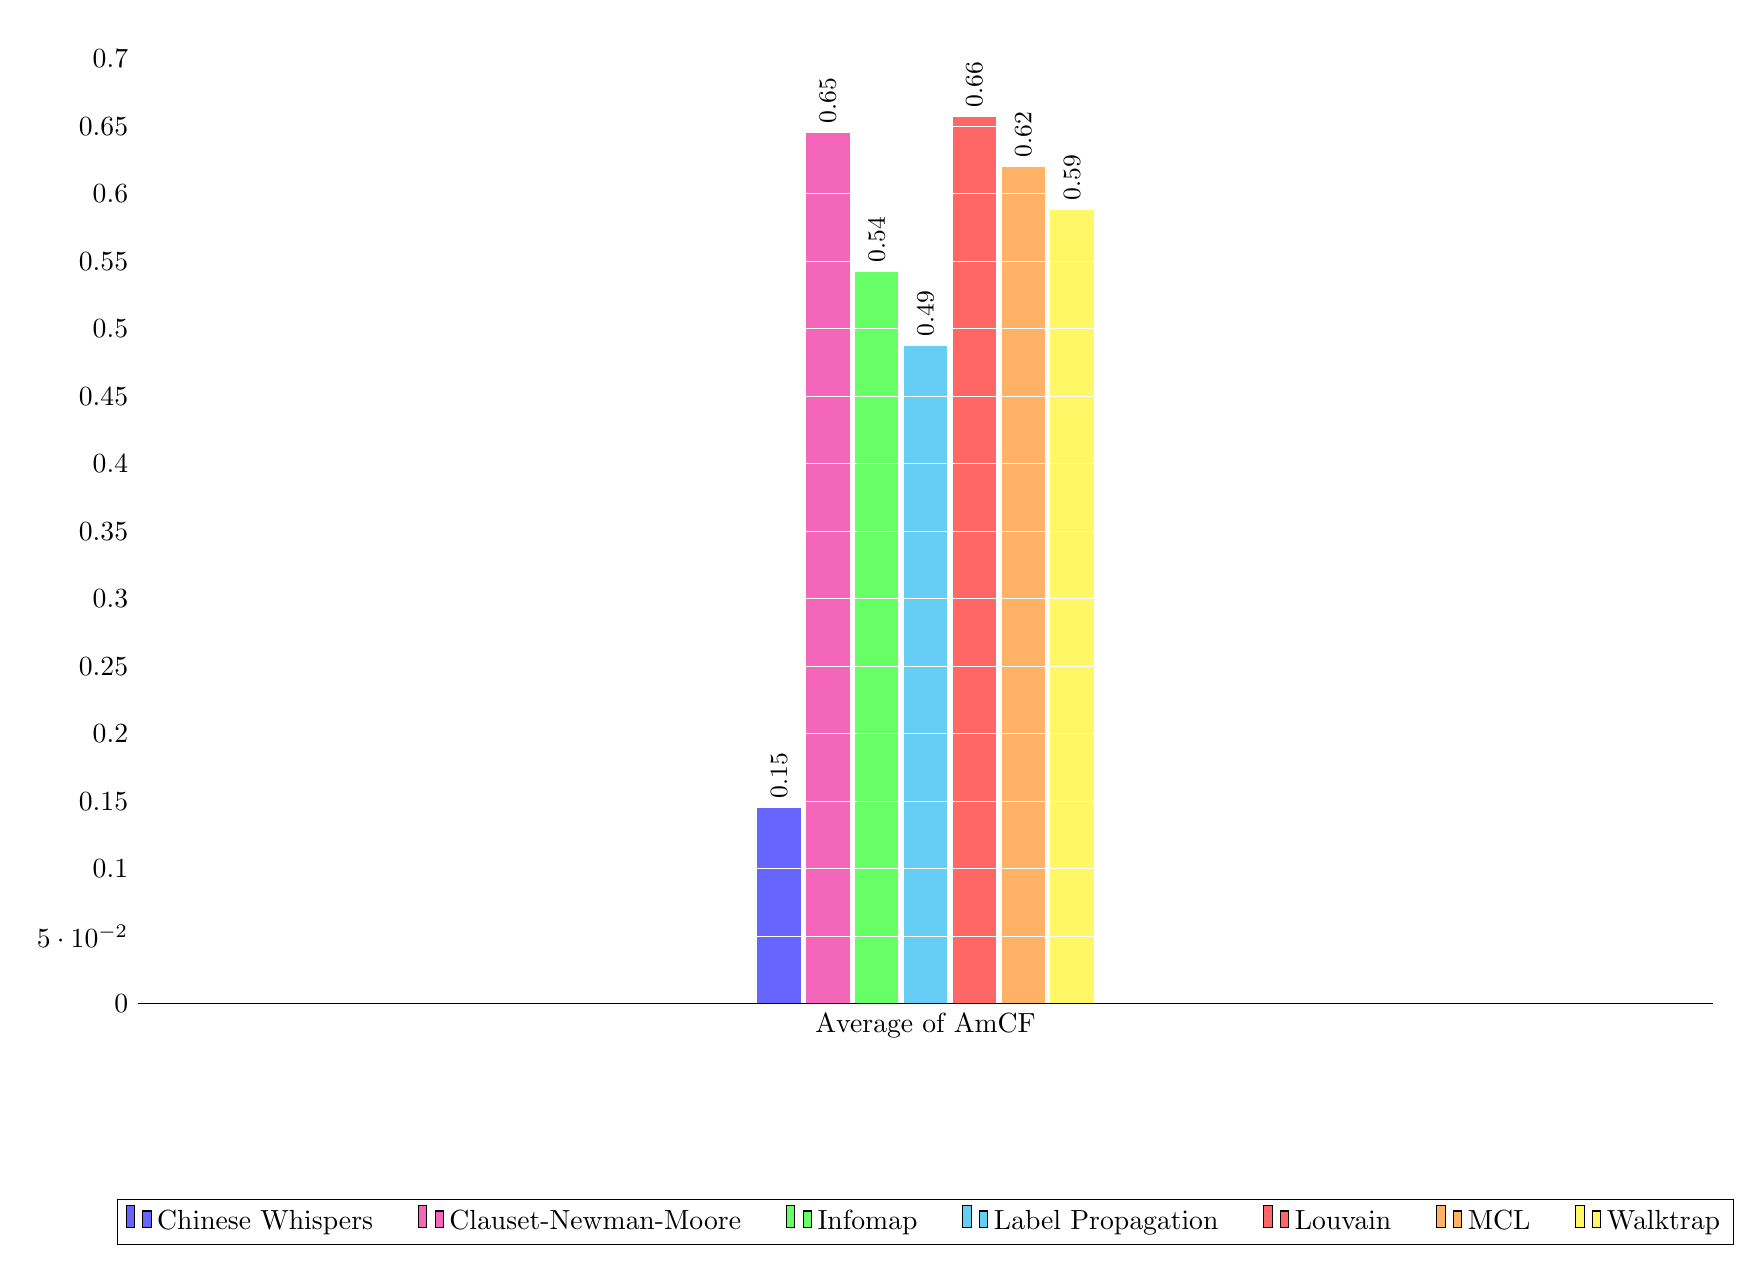
\begin{tikzpicture}
    \centering
    \begin{axis}[
        ybar, axis on top,
        height=\paperheight/2, width=\paperwidth,
        bar width=0.55cm,
        ymajorgrids, tick align=inside,
        major grid style={draw=white},
        enlarge y limits={value=.1,upper},
        ymin=0,
        axis x line*=bottom,
        axis y line*=left,
        y axis line style={opacity=0},
        tickwidth=0pt,
        enlarge x limits=0.19,
        legend style={
            at={(0.5,-0.2)},
            anchor=north,
            legend columns=-1,
            /tikz/every even column/.append style={column sep=0.5cm}
        },
        ylabel={},
        symbolic x coords={
          Average of AmCF,
        },
        xtick=data,
        nodes near coords={
            \rot{\small{\pgfmathprintnumber[precision=2]{\pgfplotspointmeta}}}
        }
    ]
    % Chinese Whispers
    \addplot [draw=none, fill=blue!60] coordinates {
      (Average of AmCF,0.145)
    };
    % Clauset-Newman-Moore
    \addplot [draw=none, fill=magenta!60] coordinates {
      (Average of AmCF,0.645)
    };
    % Infomap
    \addplot [draw=none, fill=green!60] coordinates {
      (Average of AmCF,0.542)
    };
    % Label Propagation
    \addplot [draw=none, fill=cyan!60] coordinates {
      (Average of AmCF,0.487)
    };
    % Louvain
    \addplot [draw=none, fill=red!60] coordinates {
      (Average of AmCF,0.657)
    };
    % MCL
    \addplot [draw=none, fill=orange!60] coordinates {
      (Average of AmCF,0.62)
    };
    % Walktrap
    \addplot [draw=none, fill=yellow!60] coordinates {
      (Average of AmCF,0.588)
    };
    \legend{Chinese Whispers,Clauset-Newman-Moore,Infomap,Label Propagation,Louvain,MCL,Walktrap}
    \end{axis}
\end{tikzpicture}
\end{adjustbox}
\caption{
  Plotted results of experiment Nº 3 (Part 1)
}
\caption*{\centering
  The labels represent the following metrics:
  \begin{itemize}[noitemsep]
    \item AmCF: Average Median Cluster Factor
  \end{itemize}
}
\label{fig:experiment-3.1}
\end{figure}

\begin{figure}[p]
    \centering
    \begin{adjustbox}{width=\textwidth}
    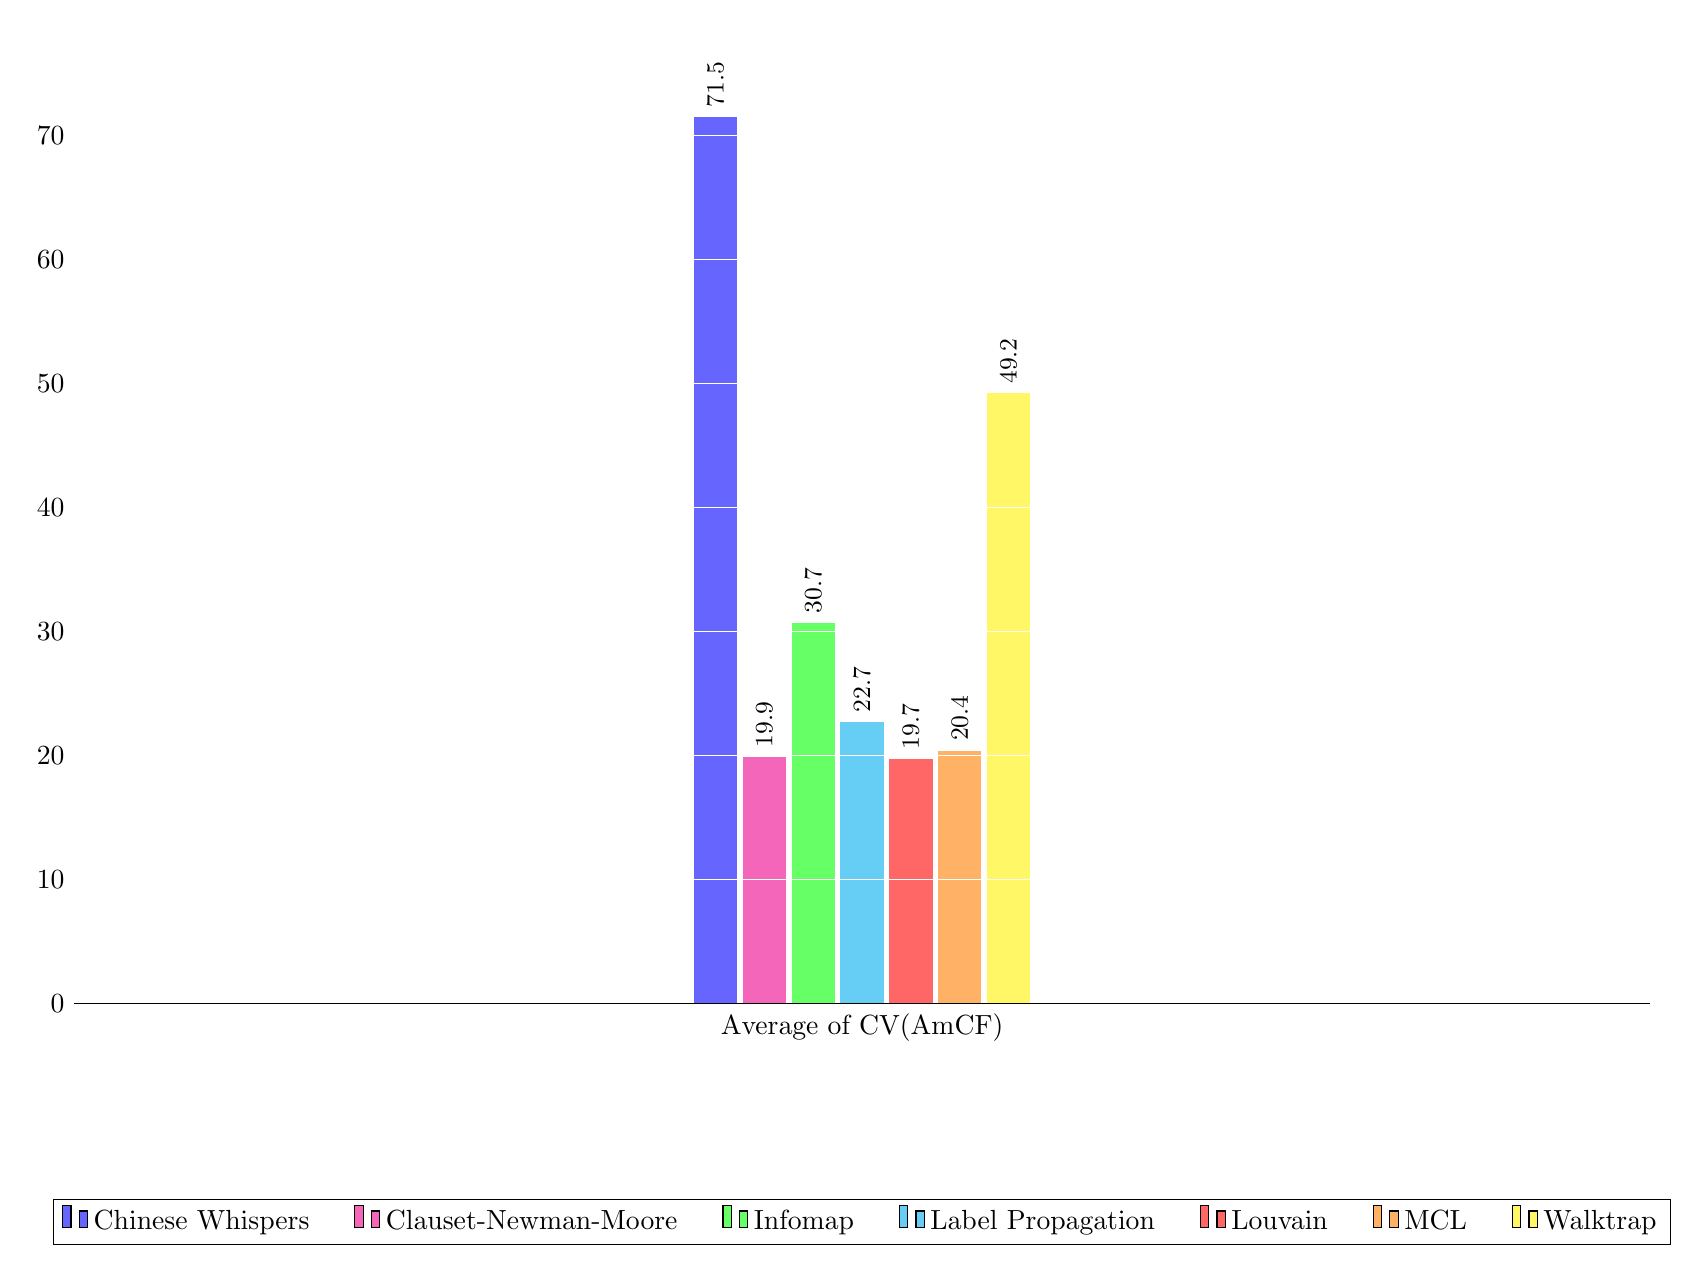
\begin{tikzpicture}
    \centering
    \begin{axis}[
        ybar, axis on top,
        height=\paperheight/2, width=\paperwidth,
        bar width=0.55cm,
        ymajorgrids, tick align=inside,
        major grid style={draw=white},
        enlarge y limits={value=.1,upper},
        ymin=0,
        axis x line*=bottom,
        axis y line*=left,
        y axis line style={opacity=0},
        tickwidth=0pt,
        enlarge x limits=0.19,
        legend style={
            at={(0.5,-0.2)},
            anchor=north,
            legend columns=-1,
            /tikz/every even column/.append style={column sep=0.5cm}
        },
        ylabel={},
        symbolic x coords={
          Average of CV(AmCF),
        },
        xtick=data,
        nodes near coords={
            \rot{\small{\pgfmathprintnumber[precision=1]{\pgfplotspointmeta}}}
        }
    ]
    % Chinese Whispers
    \addplot [draw=none, fill=blue!60] coordinates {
      (Average of CV(AmCF),71.5)
    };
    % Clauset-Newman-Moore
    \addplot [draw=none, fill=magenta!60] coordinates {
      (Average of CV(AmCF),19.9)
    };
    % Infomap
    \addplot [draw=none, fill=green!60] coordinates {
      (Average of CV(AmCF),30.7)
    };
    % Label Propagation
    \addplot [draw=none, fill=cyan!60] coordinates {
      (Average of CV(AmCF),22.7)
    };
    % Louvain
    \addplot [draw=none, fill=red!60] coordinates {
      (Average of CV(AmCF),19.7)
    };
    % MCL
    \addplot [draw=none, fill=orange!60] coordinates {
      (Average of CV(AmCF),20.4)
    };
    % Walktrap
    \addplot [draw=none, fill=yellow!60] coordinates {
      (Average of CV(AmCF),49.2)
    };
    \legend{Chinese Whispers,Clauset-Newman-Moore,Infomap,Label Propagation,Louvain,MCL,Walktrap}
    \end{axis}
\end{tikzpicture}
\end{adjustbox}
\caption{
  Plotted results of experiment Nº 3 (Part 2)
}
\caption*{\centering
  The labels represent the following metrics:
  \begin{itemize}[noitemsep]
    \item CV(AmCF): Coefficient of varition of Average Median Cluster Factor
  \end{itemize}
}
\label{fig:experiment-3.2}
\end{figure}

\begin{figure}[p]
    \centering
    \begin{adjustbox}{width=\textwidth}
    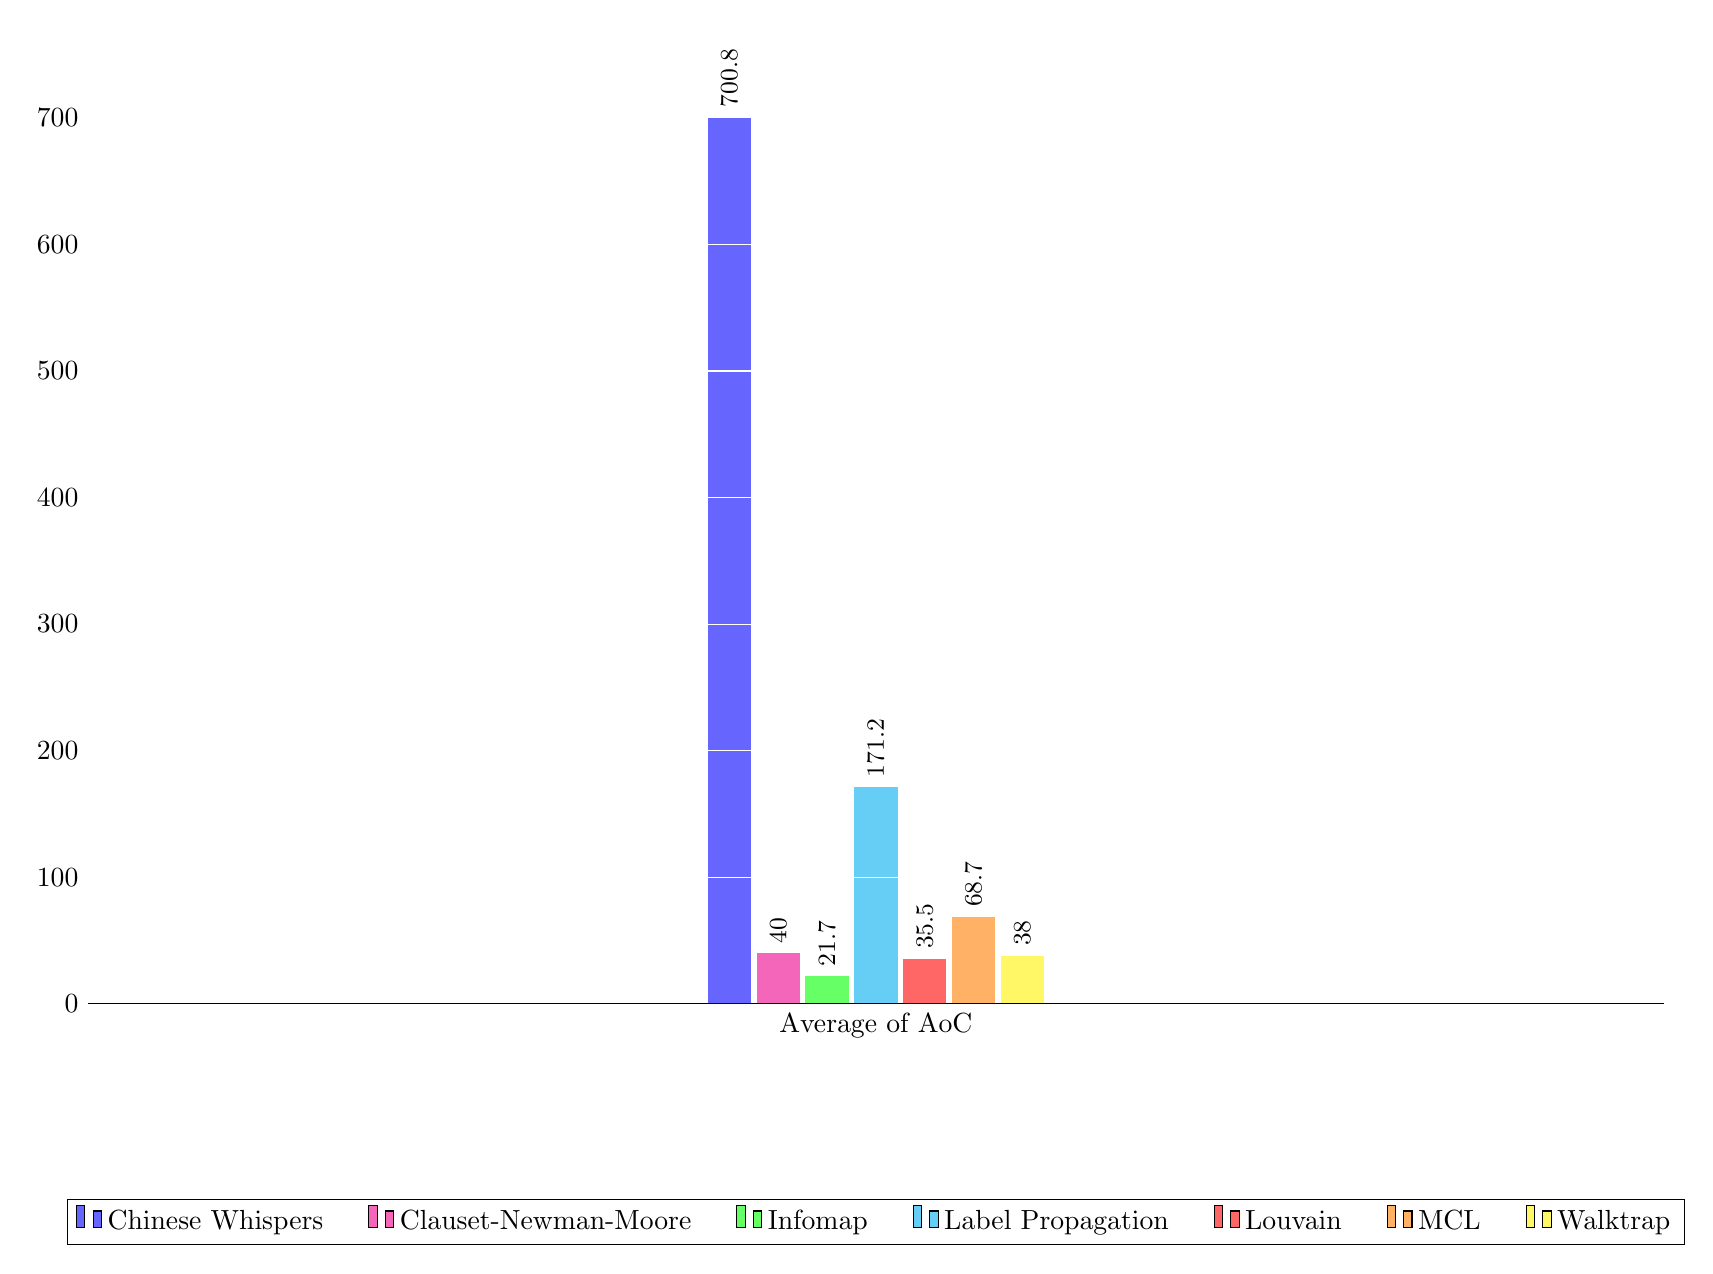
\begin{tikzpicture}
    \centering
    \begin{axis}[
        ybar, axis on top,
        height=\paperheight/2, width=\paperwidth,
        bar width=0.55cm,
        ymajorgrids, tick align=inside,
        major grid style={draw=white},
        enlarge y limits={value=.1,upper},
        ymin=0,
        axis x line*=bottom,
        axis y line*=left,
        y axis line style={opacity=0},
        tickwidth=0pt,
        enlarge x limits=0.19,
        legend style={
            at={(0.5,-0.2)},
            anchor=north,
            legend columns=-1,
            /tikz/every even column/.append style={column sep=0.5cm}
        },
        ylabel={},
        symbolic x coords={
          Average of AoC,
        },
        xtick=data,
        nodes near coords={
            \rot{\small{\pgfmathprintnumber[precision=1]{\pgfplotspointmeta}}}
        }
    ]
    % Chinese Whispers
    \addplot [draw=none, fill=blue!60] coordinates {
      (Average of AoC,700.8)
    };
    % Clauset-Newman-Moore
    \addplot [draw=none, fill=magenta!60] coordinates {
      (Average of AoC,40)
    };
    % Infomap
    \addplot [draw=none, fill=green!60] coordinates {
      (Average of AoC,21.7)
    };
    % Label Propagation
    \addplot [draw=none, fill=cyan!60] coordinates {
      (Average of AoC,171.2)
    };
    % Louvain
    \addplot [draw=none, fill=red!60] coordinates {
      (Average of AoC,35.5)
    };
    % MCL
    \addplot [draw=none, fill=orange!60] coordinates {
      (Average of AoC,68.7)
    };
    % Walktrap
    \addplot [draw=none, fill=yellow!60] coordinates {
      (Average of AoC,38)
    };
    \legend{Chinese Whispers,Clauset-Newman-Moore,Infomap,Label Propagation,Louvain,MCL,Walktrap}
    \end{axis}
\end{tikzpicture}
\end{adjustbox}
\caption{
  Plotted results of experiment Nº 3 (Part 3)
}
\caption*{\centering
  The labels represent the following metrics:
  \begin{itemize}[noitemsep]
    \item AoC: Amount of Clusters
  \end{itemize}
}
\label{fig:experiment-3.3}
\end{figure}

\begin{figure}[p]
    \centering
    \begin{adjustbox}{width=\textwidth}
    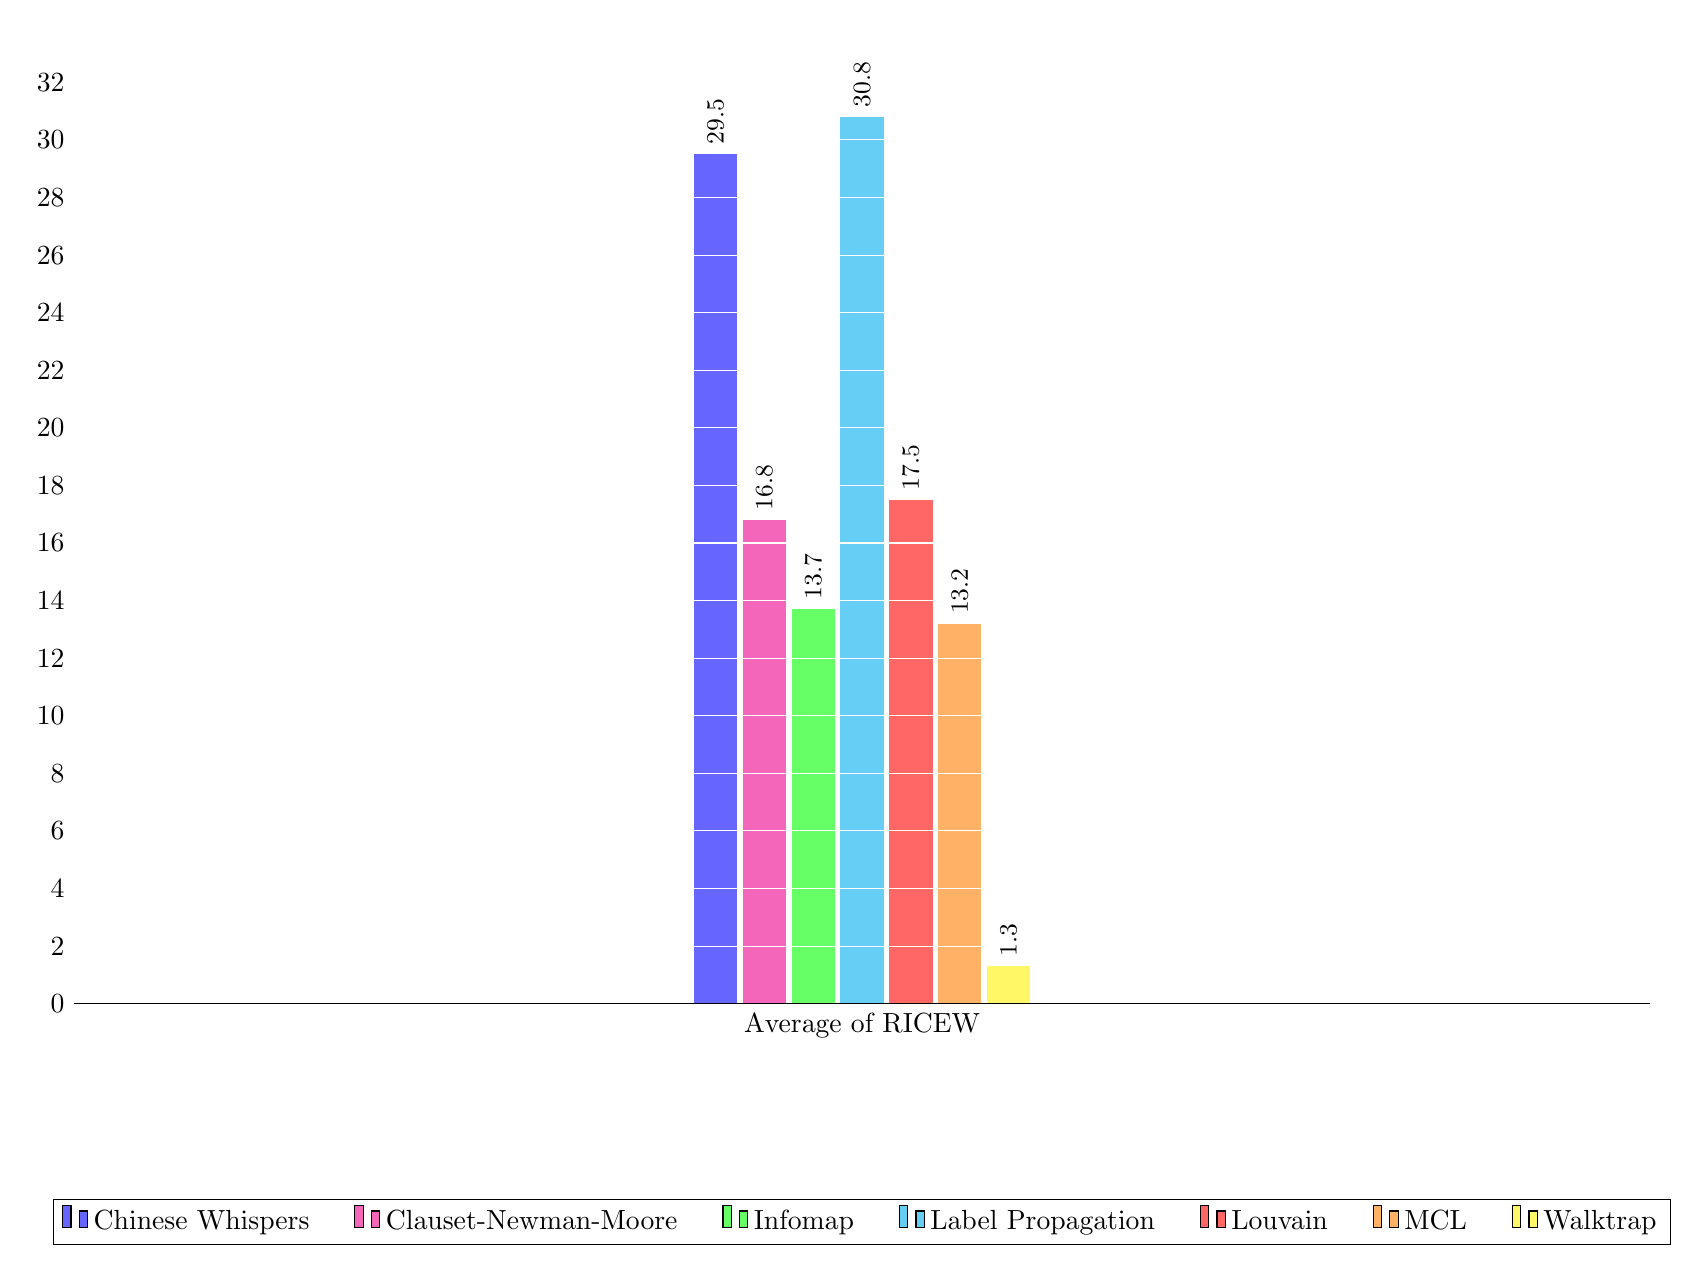
\begin{tikzpicture}
    \centering
    \begin{axis}[
        ybar, axis on top,
        height=\paperheight/2, width=\paperwidth,
        bar width=0.55cm,
        ymajorgrids, tick align=inside,
        major grid style={draw=white},
        enlarge y limits={value=.1,upper},
        ymin=0,
        axis x line*=bottom,
        axis y line*=left,
        y axis line style={opacity=0},
        tickwidth=0pt,
        enlarge x limits=0.19,
        legend style={
            at={(0.5,-0.2)},
            anchor=north,
            legend columns=-1,
            /tikz/every even column/.append style={column sep=0.5cm}
        },
        ylabel={},
        symbolic x coords={
          Average of RICEW,
        },
        xtick=data,
        nodes near coords={
            \rot{\small{\pgfmathprintnumber[precision=1]{\pgfplotspointmeta}}}
        }
    ]
    % Chinese Whispers
    \addplot [draw=none, fill=blue!60] coordinates {
      (Average of RICEW,29.5)
    };
    % Clauset-Newman-Moore
    \addplot [draw=none, fill=magenta!60] coordinates {
      (Average of RICEW,16.8)
    };
    % Infomap
    \addplot [draw=none, fill=green!60] coordinates {
      (Average of RICEW,13.7)
    };
    % Label Propagation
    \addplot [draw=none, fill=cyan!60] coordinates {
      (Average of RICEW,30.8)
    };
    % Louvain
    \addplot [draw=none, fill=red!60] coordinates {
      (Average of RICEW,17.5)
    };
    % MCL
    \addplot [draw=none, fill=orange!60] coordinates {
      (Average of RICEW,13.2)
    };
    % Walktrap
    \addplot [draw=none, fill=yellow!60] coordinates {
      (Average of RICEW,1.3)
    };
    \legend{Chinese Whispers,Clauset-Newman-Moore,Infomap,Label Propagation,Louvain,MCL,Walktrap}
    \end{axis}
\end{tikzpicture}
\end{adjustbox}
\caption{
  Plotted results of experiment Nº 3 (Part 4)
}
\caption*{\centering
  The labels represent the following metrics:
  \begin{itemize}[noitemsep]
    \item RICEW: Ratio Inter-Cluster Edge Weights
  \end{itemize}
}
\label{fig:experiment-3.4}
\end{figure}




\chapter{Discussion} \label{chap:discussion}

\section{Results}

Coming back to the introduction of this thesis and the posed research questions,
we created a full methodology that gets any monolithic software as its input,
outputting microservice candidate recommendations in various formats.
Furthermore, a large set of metrics were devised that measure the input and
output quality of said methodology.
In conclusion, we devised a methodology that improves upon similar ones in
this area of research in multiple aspects such as:

\begin{itemize}
    \item A rationale that ties the input to the output to be able to reason
    about how the generated microservice recommendations are of any relevance
    owing to the fact that the analyzed input measures common microservice
    quality metrics extracted from literature.
    \item The application of said rationale to analyzable software metrics
    that constitute the foundation of the devised methodology in the form
    of four software coupling dimensions compared to a maximum
    of two in previous research in this domain.
    \item A conducted survey of graph clustering algorithms to identify feasible
    ones via an extensive set of criteria. Eventually, seven algorithms were
    selected and incorporated into the methodology compared to a maximum
    of two in previous research in this domain. Additionally, all of these seven
    algorithms were evaluated in terms of their suitability for our methodology.
    \item A full implementation of the devised methodology with a modern
    graphical user interface that enables a user to quickly analyze input
    monolithic software.
    \item A large set of objective metrics that are numeric in nature,
    to measure the input and output of the methodology to allow for an
    easy comparison of the chosen graph clustering algorithms as well as
    the generated microservice candidate recommendations themselves.
\end{itemize}



\section{Threats to validity} \label{sect:threats-to-validity}

\paragraph{Missing dynamic coupling}
The main threat to validity was exhibited in subsection \ref{subsect:difficulties}
which is namely that the input dimension regarding the \textit{dynamic coupling}
cannot be analyzed very well in an experimental environment which decreased
the significance of our evaluation. On the other hand, using this input dimension
would have expectedly resulted in even less valid results. This problem can just
only be fully solved once our methodology is used in a production environment.

\paragraph{Shared code}
We detected that a shortcoming with our approach is that units
of an analyzed code base that are supposed to be shared (i.e. utility classes)
will be attributed to one microservice recommendation although its coupling
might be equally high toward other ones. This can be mitigated by keeping
such units in a separate top-level package or module as our methodology then
allows to ignore it in the analysis via the \code{basePackageIdentifier} parameter.
Hence, in an actual microservice decomposition one could maintain such code in a
\textit{Git Submodule} or transfer it to an internally used library that all the
microservices depend on \cite{git-submodules}.

\paragraph{Quality assessment}
Just as the other existing methodologies in this area of research
such as the ones covered in chapter \ref{chap:related}, the inherent weakness
of our methodology is to assess the quality of the generated results.
Although we devised objective metrics numeric in nature, the decision if a set
of created microservice recommendations is good is still subjective from the
standpoint of the software engineer conducting the decomposition process.
There are many possible reasons that a human could decide that certain units
of the existing application definitely should not be put into separate services
due to security concerns when a network is involved, compliance reasons, etc.
Thus, this shortcoming is also addressed in the following section on
\textit{\nameref{sect:future-work}}.



\section{Future work} \label{sect:future-work}

While the devised methodology is working and fully-functional, there are three
major improvements that were detected, with the first one being an additional
evaluation, the second one being a possible feature addition to \textit{Steinmetz},
while the last one is a follow-up on the methodology exhibited in this thesis.
In the following subsections, the three future work improvements are discussed in
further detail.

\paragraph{Evaluation study}
We detected that a useful next step would be to evaluate our methodology
with experienced software engineers and software projects that they built
or maintain. This type of evaluation would allow to corroborate the findings
of our \textit{\nameref{chap:evaluation}} as part of this thesis as an engineer
that knows the software that is getting analyzed can assess if the automated
output of our methodology matches their expectations. Additionally, we suspect
that certain patterns might be detected where our methodology falls short oftentimes
compared to the analysis of a human.

\paragraph{Manual reassignment of units to microservices candidates}
As discussed earlier already, a human software engineer might have a demur
in the decisions that \textit{Steinmetz} made. For instance, due to
security concerns or compliance reasons, the engineer might have a requirement
that certain units of the input monolithic application have to be part of
the same microservice (e.g. to avoid communication over a network).
Consequently, a feature addition to our methodology and implementation
would be that the user can select that certain units should not be divided
into separate services. This information can then be incorporated into the
analysis by the methodology when generating the microservice candidate
recommendations.

\paragraph{Automatically generating API of microservices candidates}
The other, larger follow-up improvement to our methodology is to not only
generate the microservice recommendations but to additionally generate the
API that would become necessary if the recommendations would actually be
implemented. Apart from improving the usefulness of the implementation
for a prospective user, this API generation could also be used to
automatically detect if the interfaces are efficient and effective and
to otherwise improve them by slightly shifting the boundaries between
the units, utilizing an algorithm, to offer a more holistic set of
microservice candidate recommendations that can be validated from an
additional perspective --- the quality of the interfaces between the services.




\chapter{Conclusion} \label{chap:conclusion}

The microservices paradigm is getting more and more traction while
many companies are stuck with monolithic legacy systems that could
benefit from being renovated by decomposing them into microservices.
However, legacy software is typically difficult to grasp with increasing size.
While this process is tedious and very manual for a human,
for a computer it is much easier to oversee the entirety of the
application. This area of research of this thesis is still young compared
to others in the domain of computer science as Fritzsch et al. showed in their
study on the current situation in this exact area of research.
They also concluded that more research is desired to further improve
upon existing approaches.

Thus, we showed how a rationale can tie the input to the output,
to be able to assert that the final microservice recommendations
were generated via the means of an input that leads to \textit{good}
microservice boundaries which were extracted out of the input ---
the three dimensions of coupling in the case of our methodology.
Furthermore, it became apparent that a multitude of graph clustering
algorithms are available to be utilized for creating microservice
recommendations which offered a deeper insight into which are
feasible for this purpose by leveraging the metrics that were
incorporated into our methodology which enables a user to easily
compare different graph clustering algorithms quickly to choose the
one that works the best for their input. However, we also saw that
some graph clustering algorithms consistently perform better than others.

To conclude, we devised a working methodology that generates results
in just a few minutes without any manual input,
which would have taken hours if done by a human software engineer.
Additionally, we fully implemented the devised methodology with a
modern graphical user interface that allows for fast analysis runs
that yield microservice candidate recommendations in a variety of formats
which can be used to assist human software engineers with the posed task.




% Reference lists
\newpage
\addcontentsline{toc}{chapter}{List of Figures}
\listoffigures
\newpage
\addcontentsline{toc}{chapter}{List of Tables}
\listoftables
\newpage
\addcontentsline{toc}{chapter}{Bibliography}
% Separate the sources with 'bibtopic'
\bibliographystyle{plain}
\begin{btSect}{references}
\section*{\huge{References}}
\btPrintCited
\end{btSect}
\begin{btSect}{online}
\section*{\huge{Online Sources}}
\btPrintCited
\end{btSect}

\end{document}
